\chapter[A Password Authentication Framework for the Single-Server Setting]{A Password-based Authentication Framework for the Single-Server Setting} \label{ch:vpake}

As discussed in Chapter \ref{ch:intro} using passwords for authentication is it's most common use case. 
This is usually done with the inherently flawed approach of password-over-\ac{HTML} despite the existence of more secure alternatives such as \ac{PAKE}.
In this chapter we propose a framework for cryptographic password registration and authentication, comprising a protocol for clients to register passwords in a secure way with a server while still allowing for password policies checks, as well as suitable protocols to use the registered password verifier for password-based authentication.

The first main contribution in this chapter is the definition of \ac{BPR}.
This protocol class allows a client to register a password verifier with a server without actually disclosing the password, while allowing the server to check the password's policy compliance against a password policy.
Note that this still requires a secure channel (established using for example \ac{TLS}) between client and server.
This requirement can not be removed as obtaining the password verifier eventually always leads to password disclosure.
However, this is not the goal of \ac{BPR}.
Instead, \ac{BPR} offers a way of removing the trust assumption that the server securely handles client passwords by never revealing the actual password to the server.

Using registered password verifiers to authenticate clients are the second step of the proposed framework, which can be performed using \ac{VPAKE} or \ac{tPAuth} protocols.
While \ac{VPAKE} is the first natural way of authenticating using a password on the client side and a password verifier on the server side, \ac{tPAuth} protocols can be used with verifiers as well and are more suitable for password based authentication on the web.
 
\smallskip
\noindent
This chapter is based on work in \cite{Kiefer13a,KieferM15a,DongK15a}.
 
\paragraph{Outline \& Summary of Results}
This chapter comprises 9 sections organised as follows.
Section \ref{sec:passwords} gives definitions of passwords, dictionaries, and policies, used in this chapter and Section \ref{sec:strucphash} describes a novel password hashing algorithm.
Methods introduced in these first two sections allows to convert character strings to elements usable for cryptographic operations.
Section \ref{sec:zkppc} introduces the notion of \acp{ZKPPC} and how it can be used to build password registration protocols from it.
The resulting notion of \ac{BPR} is formalised in the subsequent Section \ref{sec:bpr} giving a security model and an efficient protocol.
Section \ref{sec:spc-bpr} introduces an alternative approach to \ac{BPR} based on set theory.
To compare the different \ac{BPR} approaches Section \ref{sec:performance} provides implementations for all three approaches and gives a comparison of the protocols and their security guarantees.
This concludes the password registration step of the framework.
To use passwords registered with one of the \ac{BPR} protocols described in Section \ref{sec:zkppc}-\ref{sec:spc-bpr}, Sections \ref{sec:pake} discusses and proposes appropriate \ac{PAKE} and \ac{VPAKE} protocols.
The chapter is concluded by the description of an online demo for the proposed framework in Section \ref{sec:vpake-demo} that demonstrates how to use the proposed protocols in practice and Section \ref{sec:vpake-conclusion} to summarise the results of this chapter.

\section{Modelling Passwords and Policies} \label{sec:passwords}

In the following we describe how to model passwords, dictionaries they are chosen from, and password policies. 
Password strings have to be mapped to integers before they are used in cryptographic operations. 
For our purposes such an integer mapping must be able to preserve the password structure. 
In particular, the way a password string is composed from single characters must remain visible from the resulting integer value. 
As part of password modelling we describe an appropriate encoding scheme that maps password strings defined over the alphabet of printable \ac{ASCII} characters to integers while preserving their structure. 
We further model and define password policies as some kind of regular expressions over different \ac{ASCII} character sets.
In addition to the main model we describe an alternative way of modelling that is used in Section \ref{sec:spc-bpr}

\subsection{Password Strings and Dictionaries}
We consider \emph{password strings} $\pwd$ over the \emph{\ac{ASCII}  alphabet} $\Sigma$ containing all 94 \emph{printable} \ac{ASCII}  characters.
Although we do not consider password strings consisting of other characters, our approach is easily adaptable to \ac{UTF-8} and other character sets.
We split $\Sigma=d\cup u\cup l\cup s$ into four subsets:
\begin{itemize}
	\item set of \emph{\bf digits} $d=[0-9]$ (or \ac{ASCII}  codes $[48-57]$),
	\item set of \emph{\bf upper case letters} $u=[A-Z]$ (or \ac{ASCII}  codes $[65-90]$)
	\item set of \emph{\bf lower case letters} $l=[a-z]$ (or \ac{ASCII}  codes $[97-122]$)
	\item set of \emph{\bf symbols} $s=[$!\textquotedbl\#\$\%\&'()*+,-./~:;\textless=\textgreater?@~[\textbackslash]\^{}\_`~\{\textbar\}\textasciitilde$]$ (or \ac{ASCII}  codes $[33-47,58-64,91-96,123-126]$)
\end{itemize}

\noindent
By $\cD$ we denote a \emph{general dictionary} containing all strings that can be formed from printable \ac{ASCII}  characters, \ie all power sets of $\Sigma$.
A \emph{password string} $\pwd=(c_{0},\dots,c_{n-1})\in\Sigma^n\subset\cD$ of length $n$ is an ordered set of characters $c_i\in\Sigma$.

\subsection{Password Mapping --- From Strings to Integers}\label{sec:pwdencoding}
In the following we show how a password string $\pwd$ can be mapped to an integer $\pi$ for further cryptographic processing in a way that preserves the character composition of $\pwd$ and makes it possible to efficiently reconstruct $\pwd$ from $\pi$. 

%We define the encoding in the following with a variable base $b$ and discuss possible choices for it in Remark \ref{rem:basischoice} at the end of Section \ref{sec:strucphash}.
%Note that the choice of base $b=95$ in the proceedings version of this work \cite{KieferM14b} renders the password hashing protocol in Section \ref{sec:strucphash} insecure.

\subsubsection{Mapping of Password Characters to Integers}
In order to preserve the character structure of a password string $\pwd$ upon its mapping to an integer we first define a \emph{character mapping} function $\chrint:\Sigma\mapsto\ZZ_{95}$ for any printable \ac{ASCII}  character $c\in\Sigma$ that internally uses its decimal \ac{ASCII}  code $\ASCII(c)$ to output an integer in $\ZZ_{95}$:
\[
\chrint(c) =
\left\{
	\begin{array}{ll}
		\bot  & \mbox{if } \ASCII(c) < 32 \\
		\ASCII(c)-32 & \mbox{if } 33 \leq \ASCII(c) \leq 126 \\
		\bot & \mbox{if } 126 < \ASCII(c)
	\end{array}
\right.
\]


\subsubsection{Position-Dependent Mapping of Password Characters to Integers}
A printable \ac{ASCII}  character $c\in\Sigma$ may appear at any position $i\in[0, n-1]$ in a password string $\pwd\in\Sigma^n$. For every position $i$ we require a different integer to which $c_i\in\pwd$ can be mapped to.
Assuming a reasonable upper bound $\pmax$ on the password length $n$, \ie $n\leq \pmax$, and some \emph{shift base} $b\in\NN$, we define four integer sets $\Omega_x$, $x\in\Sigma' = \{d, u, l, s\}$, where $d$, $u$, $l$, $s$ are the identifiers of the four \ac{ASCII}  character subsets that were used to define $\Sigma$ as follows:
\begin{itemize}
	\item $\Omega_d = \{b^i\chrint(c)\}$ for all digits $c\in d$ and $i=0,\ldots,\pmax-1$. Note that $|\Omega_d|= 10\pmax$.
	\item $\Omega_u = \{b^i\chrint(c)\}$ for all upper case letters $c\in u$ and $i=0,\ldots,\pmax-1$. Note that $|\Omega_u|= 26\pmax$.
	\item $\Omega_l = \{b^i\chrint(c)\}$ for all lower case letters $c\in u$ and $i=0,\ldots,\pmax-1$. Note that $|\Omega_l|= 26\pmax$.
	\item $\Omega_s = \{b^i\chrint(c)\}$ for all symbols $c\in s$ and $i=0,\ldots,\pmax-1$. Note that $|\Omega_s|= 32\pmax$.
\end{itemize}
Any password character $c_i\in\pwd$, $i\in[0,\pmax-1]$ can therefore be mapped to one of the four sets $\Omega_x$, $x\in\Sigma'$ with the \emph{position-dependent character mapping} function $\ichrint:\Sigma\mapsto\Omega_{x}$, defined as
\[
\ichrint(c, i)= b^i\chrint(c),
\]
where the shift base $b\in\NN$ is a public constant.
We write $\pi_i \gets \ichrint(c, i)$ for the integer value of the $i$th character $c_i\in\pwd$.
%Let $\Omega_\Sigma=\Omega_d\cup\Omega_u\cup\Omega_l\cup\Omega_s$.

\subsubsection{Mapping of Password Strings to Integers}


A \emph{password mapping} function $\pwdint:\Sigma^n\mapsto\ZZ_{b^{\pmax}}$ that maps any password string $\pwd=(c_{0},\dots,c_{n-1})\in\Sigma^n$ to an integer in a larger set $\ZZ_{b^{\pmax}}$ in a way that preserves the $i$th position of each character $c_i$ is defined as follows:
\[
\pwdint(\pwd) = \sum_{i=0}^{n-1}b^{i} \chrint(c_{i}) = \sum_{i=0}^{n-1}\ichrint(c_i, i) \textrm{ for } c_i\in\pwd
\]
We will use $\pwd$ to denote a password string and $\pi \gets \pwdint(\pwd)$ for its integer value. Note that $\pi = \sum_{i=0}^{n-1}\pi_i$. %The special constant $\emptyset$ is used to denote zero and $\emptyset$ is not a valid password character.
The mapping computed through $\pwdint$ is injective and reversible. For example, $\pi = 883318$ with $b=100$ is the integer value of password string $\pwd = (\textrm{2},\textrm{A},\textrm{x})$. The string can be recovered by concatenation of $883318\mod 100=18~ \widehat{=}$ 2 at position 0, $(797353\mod 100^2)-(797353\mod 100)=3300=33\cdot 100^1~ \widehat{=}$ A at position $1$ and $797353-(797353\mod95^2)=880000=88\cdot 100^2~ \widehat{=}$ x at position $2$.



\subsection{Password Policies}\label{sec:policies}
A password policy is defined to impose requirements on password complexity in terms of the minimum number of characters, minimal number of character classes, and minimal number of characters in each class.
A \emph{password policy} $f=(R,\pmin,\pmax)$ is modelled using some sort of \emph{regular expression} $R$ over $\Sigma'=\{d, u, l, s\}$, a \emph{minimum length} $\pmin$ and a \emph{maximum length} $\pmax$ that a password string $\pwd$ must fulfil.
The way password policies are modelled in this work is suitable for policies that put restrictions on the password length and the nature of password characters. Other types of policies, \eg search for natural words in a password (cf.~Dropbox password-meter, \url{https://tech.dropbox.com/2012/04/zxcvbn-realistic-password-strength-estimation}) are currently not supported by our framework and thus left for future work.
We write $f(\pwd)=\true$ to indicate that the policy is satisfied by the password string \pwd.
%The upper limit $n$ can be picked such that sufficiently long passwords are admitted and will have impact on the efficiency of the corresponding zero-knowledge proofs for policy compliance.
For example, %The following examples illustrate how regular expressions $R$ should be used to define policies:
\begin{itemize}
	\item $f=(\mathtt{ds}, 6, 10)$ means that $\pwd$ must have between 6 and 10 characters with at least one digit and one symbol.
	\item $f=(\mathtt{uss}, 8, 12)$ means that $\pwd$ must have between 8 and 12 characters with at least one upper-case letter and two symbols.
	\item $f=(\mathtt{duls}, 8, 16)$ means that $\pwd$ must have between 8 and 16 characters with at least one character of each type.
\end{itemize}

\noindent
A character $c_i\in\pwd$ is called \emph{significant} if it is necessary to fulfil a policy expression $R$ and say the according set $R_j\in R$ is the according \emph{significant set}.
For every $R_j\in R$ the first occurrence of a character $c_i\in R_j$ is considered significant.
Note that $\Sigma$, and thus $d,u,l$ and $s$, in this work can refer to the set of encoded characters, or the set of \ac{ASCII}  characters, depending on the context.

\begin{remark}
Note that in practice password policies do not specify \pmax. 
We leave it for the server administrator to decide whether \pmax should be mentioned explicitly in $f$ or fixed in the system to allow for all reasonable password lengths.
A password policy is called simplified if \pmax is omitted, \ie a simplified policy is given by $f=(R,\pmin)$.
\end{remark}

% \subsubsection{Simplified Password Policies}
% A \emph{password policy} is defined as a tuple $f=(R,\pmin)$, where $R$ is a policy expression over $\Sigma=\{d, u, l, s\}$, where $d$ denotes digits, $u$ upper case letters, $l$ lower case letters, $s$ symbols, and \pmin defines the minimum length of a password.
% We do not specify an upper limit on the password length in this simplified password policy.
% A policy expression $R$ over $\Sigma$ is a simplified regular expression that only specifies the sets necessary for a string to fulfil the expression.
% In particular, it specifies the minimum number of occurrences of elements from $\Sigma$ in the password string, e.g., $R=dl$ requires \pwd to have at least one digit and one lower case letter, and $R=ssd$ requires \pwd to have at least two symbols and one digit.
% We write $f(\pwd)=\true$ to indicate that the policy is satisfied by the password string \pwd.

\subsection{An Alternative Definition}\label{sec:spc-passwords}
Instead of the previously described definition of passwords and policies we propose an alternative description that giving a set-theoretical approach.
Note that only the mapping of passwords to cryptographic elements and the policy definition changes, \emph{not} the definition of dictionaries, character sets, or passwords.

\subsubsection{An Alternative Policy Definition} \label{sec:lsss}
An alternative approach of defining password policies is a set-theoretical representation, \ie \emph{monotone access structures} \cite{ito89}.
Note that this approach is more general than only for passwords.
We describe in the following paragraph how the alternative password mapping and policy description is defined for the special case of password policies.
A policy $f$ defines a pair $(\cS,\Gamma_\cS)$ where \cS is a set and $\Gamma_\cS$ is an access structure over \cS. 
The access structure is a subset of the powerset $2^\cS$. 
We say an access structure $\Gamma_\cS$ is monotonic if for each element in $\Gamma_\cS$, all its superset is also in $\Gamma_\cS$. 
We say a set \cC satisfies a policy $f$, written as $f(\cC)=\true$, if $\cC\in \Gamma_\cS$. 
A set \cC that satisfies $f$ is called an authorised set. 
Access structures capture many complex access control and authorisation policies. For example, $\cS$ can be a set of credentials and $\Gamma_\cS$ defines subsets of credentials that are required for authorisation.

It has long been known that an access structure can be mapped to a \ac{LSSS} \cite{ito89,bei96}. 
Given an access structure $\Gamma_\cS$ defined over $\cS$, one can choose a secret and split it into a set of shares accordingly. 
Each share is associated with an element in $\cS$ and the following holds: 
(1) any set of shares can reconstruct the secret if the elements associated with the shares form an authorised set, and 
(2) any set of shares does not reveal any information about the secret if the elements associated with the shares do not form an authorised set.
In this way, checking whether a set satisfies a policy is equivalent to checking whether a set of shares can reconstruct the secret. 
There are several generic approaches to map access structures to \ac{LSSS}, in this paper we will use the \ac{MSP} approach introduced by \citet{bei96}. 

\subsubsection{Alternative Password Mapping}
% In this paper, we consider a password to be in the basic format of a finite length string of printable characters (\ac{ASCII} , \ac{UTF-8}, etc.). 
% We do not consider other forms of passwords such as graphical passwords \cite{suo05}. 
% It is a common practice to partition the password alphabet into character classes, e.g., upper case, lower case, symbols and digits. 
% These character classes can be seen as disjoint subsets of the alphabet. 
% % Another common feature of password policies is a minimum number of characters a password must provide.
% For example, every valid password must have at least one character from each class and eight characters overall.
% %Let $P=(\min,\{t_i, A_i\})$ thus denote a password policy with minimum password length \min and a set of threshold, character set pairs.

An alternative approach of mapping passwords to cryptographically usable elements is given in the set theoretical setting.
To this end we first define a mapping from passwords (character strings) to a set, which can be used in cryptographic set operations.
First we observe that passwords are arbitrary strings and as such can have repeated characters. 
So the collection of characters in a password forms a multiset, not a set. 
The problem is that some direct conversion from a character multiset (password) to a set results in lost characters.
For example, if client chooses ``pa\$\$w0rd'', the resulting set would be $\{p,a,\$,w,0,r,d\}$.
This can be solved by pre-processing the characters in the dictionary and passwords.

The dictionary pre-processing step converts the dictionary into a set that can later be used in the password registration protocol. 
This step is done by the server as follows. 
Let $\Sigma=\sigma_1\cup\dots\cup \sigma_m$ be the alphabet where $\sigma_i$ is a character class (digits, lower case, etc.). 
The server transforms it into $\Sigma'$ based on password policy $f$. 
For each $\sigma_i$, there is a threshold $t_i$ in policy $f$ that says at least $t_i$ characters from $\sigma_i$ need to appear in the password. 
If $t_i = 0$, then the serve just skips all characters in this class $\sigma_i$ because they do not have to be checked. 
Otherwise, the server creates an empty set $\sigma'_i$, appends an index (from $1$ to $t_i$) to each character in $\sigma_i$, and puts the $t_i$ copies of indexed characters into $\sigma'_i$. 
For example, if $\sigma_i=l$ contains lower case characters and $t_i=2$, then $\sigma'_i=\{a1,a2,b1,b2,\ldots,z1,z2\}$. 
The union of $\sigma_i$ builds the set $\Sigma'$ to be used later 
This step has to be done only once as long as policy $f$ does not change.

The password pre-processing is performed as follows. 
We define a function $\psi$ for the client to convert a password (character string) into a set. 
For the $i$th character in the password, the function creates a substring of the password including the first $i$ characters in the password. 
Then the function appends to the $i$th character the number of occurrence of itself in the substring and puts the result into a set. 
For example, ``pa\$\$w0rd'' will be converted into $\{p1,a1,\$1,\$2,w1,01,r1,d1\}$. 
 


\subsection{Password Distributions and Min-Entropy} \label{sec:min-entropy}
Intuitively, a password hashing scheme should be considered secure if an attacker can not retrieve the password from its hash more efficiently than by performing a brute-force attack over the dictionary. 
Therefore, security definitions for password hashing or dictionary attack resistance rely on a notion of guessability, here min-entropy $\beta$.

The dictionary $\cD$, from which passwords are chosen, has min-entropy $\beta$ such that efficient sampling of the dictionary allows guessing a password with probability in $\beta$.
Although passwords in cryptographic research are often assumed to be uniformly at random distributed low-entropy secrets, we consider this somewhat more realistic password model for password registration.
In particular, we consider passwords to be character strings where the distribution of characters depends on the used character sets $\omega$, character positions and the password string itself.
We thus use a definition of password min-entropy commonly used in password security research \cite{ShayKKLMBCC10,KomanduriSKMBCCE11,MazurekKVBCCKSU13}, which captures the difficulty of brute-force attacks on passwords chosen from certain dictionaries.
As discussed in \cite{ShayKKLMBCC10,KomanduriSKMBCCE11}, this definition can capture many realistic password creation models.
Let $\DD_\omega$ denote the probability distribution in password \pwd of characters from a character set $\omega\in\{\Sigma,d,u,l,s\}$.
Min-entropy for $\pwd=(c_0,\dots,c_{n-1})$ is then defined according to \citet{shannon48} as
\[
  \beta_{\cD_{f,l}} = -\max_{\pwd\in \cD_{f,l}} \sum_{i=0}^{n-1} [\DD_\Sigma(c_i)\lg(\DD_\Sigma(c_i))].
\]
Note that definitions for min-entropy of $\cD$ and $\cD_f$ are equivalent to the definition for $\cD_{f,l}$.
While this may be surprising at first glance, one has to consider that while the policy restricts the character space, it does not restrict the positions where these characters appear, \ie an adversary cannot exclude any characters at any position.\footnote{Note that we exclude the special case where every character in a password is significant and the policy expression $R$ does not use all four available character sets. Changes for these can be easily incorporated.}

% We define the probability distribution $\DD_\omega$ of a character set $\omega\in\{\Sigma,d,u,l,s\}$ at position $i$ in password $\pwd=(c_0,\dots,c_{n-1})$ as $\DD_\omega=\Pr[c_i | i \wedge \pwd \wedge c_i\in\omega]$.
% Definition of the condition $i \wedge \pwd \wedge c_i\in\omega$ in the probability is left open for future work.
% This allows us to define min-entropy of a dictionary $\cD$, or in our case of $\cD_{f,l}$.
% Let $\DD_{\cD_{f,l}}=\Pr[\pwd]$ denote the password distribution in a dictionary $\cD_{f,l}$.
% Min-entropy $\beta_{\cD_{f,l}}$ of the dictionary is then given by $\beta_{\cD_{f,l}}=\min_{\pwd\in\cD_{f,l}} \log_2 (1/\DD_{\cD_{f,l}})$.
% In particular
% %, $\min_{\pwd\in\cD_f} \log_2 (1/\Pr_\DD[\pwd])$ and $\min_{\pwd\in\cD_{f,l}} \log_2 (1/\Pr_\DD[\pwd])$ respectively.
% % Min-entropy for $\cD_{f,l}$ is therfore given by
% \[
% \beta_{\cD_{f,l}} = \min_{\pwd\in \cD_{f,l}} \log_2 \left(\left( \prod_{i=0}^{n-1} \DD_{\Sigma}\right)^{-1}\right). %\Pr_{\DD_{\Sigma}}[c_i | i \wedge \pwd \wedge c_i\in\omega]
% \]
% % where $\DD_\Sigma$ is the distribution of \ac{ASCII}  characters and $\pwd=(c_0,\dots,c_{n-1})$.
% % The problem with this definition as $\beta_\cD$ is with less than $6.6$ very small.
% % This is due to the missing minimum length in $\cD$.
% % Therefore, to get a useful definition, we consider only $\cD_l$ where passwords have a minimum length of $l$ characters.
% In this case $\beta_{\cD_l}$ can has an upper bound of $\log_2(94^l)$ for uniformly at random distributed characters.
% % We further have dictionaries $\cD_f$ and $\cD_{f,l}$ with $f=(R,\pmin)$ and $l\geq\pmin$.
% % The regular expression $R$ defines which character sets from $\Sigma$ have to be present in every $\pwd\in\cD_f$, while $n$ gives a minimum size.
% % While these dictionaries have a different definition, their min-entropy is equivalent to $\cD$ (with according length restrictions).
% %, \ie the min-entropy is given by $\beta_{\cD_{f,l}} \leq \log_2(94^{l-m} \cdot \prod_{i=1}^{m} |R_i|)$.

\begin{remark}
Defining how character properties influence the distribution \DD of characters and therefore passwords and what are these exact properties, \eg password length, neighbouring characters, character distribution in a language etc., is out of scope of this work.
Further, although min-entropy seems a reasonable measure for modelling dictionary attack resistance of \ac{BPR} protocols,
we stress that min-entropy alone might not be sufficient to estimate the real password strength. 
As shown by \citet{MazurekKVBCCKSU13}, password strength is a complex matter (due to a variety of real-world attacks) and can hardly be captured through a single metric like min-entropy.
%We therefore stress that the definition of min-entropy is not necessarily equivalent to password strength.
%But this is not the focus of this work and may be worth exploring in future in order to refine security guarantees.
% However, note that our model can be easily extended to capture other, more complex metrics.
% While this work is concerned with the question how to efficiently perform blind password registrations with policy checks, we have to consider a certain type of password entropy.
\end{remark}

\subsection{Password Verifiers}
Password verification information stored by a server are denoted \ver and defined as follows.
\begin{itemize}
  \item $\phi(\pwd, r)$ on input of password \pwd and randomness $r$ deterministically outputs a password verifier \ver.
\end{itemize}
Note that \ver always has the form $(H, r)$ where $r$ is the randomness input into $\phi$ and $H$ is some function of \pwd and $r$.
In particular, the verifier \ver stored by the server is sufficient to authenticate a user holding only password \pwd and $H$ can be computed when \pwd and $r$ are known.

\mynote{use this \ver everywhere ...}

%****************** Randomised Password Hashing ****************************

\section{Randomised Password Hashing} \label{sec:strucphash}
A \emph{password hashing} scheme $\Pi$ that is used to compute password verification information \ver for later use in \ac{VPAKE} protocols is defined as follows, extending the definition introduced by \citet{BenhamoudaP13}:

\begin{itemize}
	\item $\PSetup(\secpar)$ generates password hashing parameters \paramP. 
	  These parameters contain implicit descriptions of random salt spaces $\mathbb{S}_P$ and $\mathbb{S}_H$.
	\item $\PPHSalt(\paramP)$ generates a random pre-hash salt $s_P\rin\mathbb{S}_P$.
	\item $\PPreHash(\paramP, \pwd, s_P)$ outputs pre-hash value $P$.
	\item $\PHSalt(\paramP)$ generates a random hash salt $s_H\rin\mathbb{S}_H$.
	\item $\PHash(\paramP, P, s_P, s_H)$ outputs hash value $H$.
\end{itemize}

\noindent
In the above syntax the algorithm $\PPreHash$ is \emph{randomised} with a pre-hash salt $s_P$, which extends the notion proposed by \citet{BenhamoudaP13}, where $\PPreHash$ is deterministic (and realised in constructions as a random oracle output $\RO(\pwd)$). 
In contrast we are interested in algebraic constructions of both $\PPreHash$ and $\PHash$ to allow for efficient proofs of knowledge involving pre-hash value $P$. 
The randomisation of $\PPreHash$ further increases the complexity of an offline dictionary attack that recovers $\pwd$ from $P$ since it removes the ability of an attacker to pre-compute pairs $(P,\pwd)$ and use them directly to recover $\pwd$ (see also Section~\ref{sec:pwreg}). 
We write $H\gets \HashP(\pwd,r)$ to denote $H\gets \PHash(\paramP,P,s_P$, $s_H)$ with $P\gets\PPreHash(\paramP,\pwd,s_P)$, where $r=(s_P,s_H)$ combines the randomness used in \PHash and \PPreHash. 
A secure $\Pi$ must satisfy the following security properties. 
Note that password-hiding is a new property introduced here to ensure that password hashes $H$ do not leak any information about \pwd. 
The remaining four properties are from \cite{BenhamoudaP13}, updated where necessary to account for the randomised $\PPreHash$:

\begin{itemize}
  \item Password hiding: 
    For all \ac{PPT} algorithms $\cA=(\cA_1,\cA_2)$ where $\cA_1$ on input $\paramP\gets\PSetup(\secpar)$ outputs two equal-length password strings $\pwd_0$ and $\pwd_1$, $\cA_2$ on input $H\gets\PHash(\paramP,P,s_P,s_H)$, where $s_H\gets\PHSalt(\paramP)$, $s_P\gets\PPHSalt(\paramP)$, and $P\gets\PPreHash(\paramP,\pwd_b, s_P)$ for a random bit $b\rin\bits$ outputs bit $b'$ there exists a negligible function $\varepsilon(\cdot)$ such that
$|\Pr[b'=b]-\frac12|\leq\varepsilon(\secpar)$.

  \item \textbf{Pre-image resistance:}
    For all \ac{PPT} algorithms \cA running in time at most $t$, there exists a negligible function $\varepsilon(\cdot)$ such that
    \[\Pr[(i,P)\gets \cA^{\HashPO(\cdot), \Verify(\cdot)}(\paramP);~ \Verify(i,P) = 1]\leq \frac{\alpha t}{2^\beta t_\PPreHash}+\varepsilon(\secpar),\]
    for small $\alpha$ and $t_\PPreHash$ being the running time of \PPreHash, with $\paramP\gets\PSetup(\secpar)$.
    \begin{itemize}
      \item Each $i$th invocation of $\HashPO(\cdot)$ returns $(H,s_H)$ with $H\gets\PHash(\paramP,P,s_P,s_H)$ and stores $T[i]\gets\PPreHash(\paramP,\pwd, s_P)$, where $s_H\gets\PHSalt(\paramP)$, $s_P\gets\PPHSalt(\paramP)$, and $\pwd\rin\cD$.
      \item \Verify(i, P) allows \cA to check whether whether his guess is correct, \ie it returns $1$ iff $T[i]=P$, $0$ otherwise. 
    \end{itemize}
%     $\Finalise(i,P)$ returns $1$ iff $T[i]=P$, $0$ otherwise. 
%     (Note that $\HashPO(\cdot)$ does not return $s_P$.)

\item \textbf{Second pre-image resistance:}
    For all \ac{PPT} algorithms \cA there exists a negligible function $\varepsilon(\cdot)$ such that for $P'\gets \cA(\paramP, P, s_H)$
      \[\Pr[P'\not=P \wedge \PHash(\paramP,P,s_H)=\PHash(\paramP,P',s_H)] \leq \varepsilon(\secpar),\]
      with $\paramP\gets\PSetup(\secpar), s_P\gets\PPHSalt(\paramP), s_H\gets\PHSalt(\paramP)$ and $P\gets\PPreHash$ $(\paramP, \pwd, s_P)$ for any $\pwd\in\cD$.

\item \textbf{Pre-hash entropy preservation:}
    For all polynomial time samplable dictionaries \cD with min-entropy $\beta$, and any \ac{PPT} algorithm \cA, there exists a negligible function $\varepsilon(\secpar)$ such that for $(P,s_P)\gets \cA(\paramP)$ with $\paramP\gets\PSetup(\secpar)$ and random password $\pwd\rin\cD$:
      \[\Pr[s_P\in\SSS_P \wedge P=\PPreHash(\paramP,\pwd,s_P)] \leq 2^{-\beta} + \varepsilon(\secpar).\]

\item \textbf{Entropy preservation:} 
    For all polynomial time samplable dictionaries $\cD$ with min-entropy $\beta$, and any \ac{PPT} algorithm \cA, there exists a negligible function $\varepsilon(\secpar)$ such that for $(H,s_P,s_H)\gets \cA(\paramP)$
      \[\Pr[s_P\in\SSS_P \wedge s_H\in\SSS_H \wedge H=\HashP(\paramP,\pwd,s_P,s_H)] \leq 2^{-\beta} + \varepsilon(\secpar),\]
      where $\paramP\gets\PSetup(\secpar)$ and $\pwd\rin\cD$.
\end{itemize}

\subsection{Password Hashing from Pedersen Commitments}\label{sec:pwhashped}
We introduce a new randomised password hashing scheme $\Pi=(\PSetup,\PPHSalt,\allowbreak\PPreHash,\allowbreak\PHSalt$, $\PHash)$ for \ac{ASCII}-based passwords using Pedersen commitments. 
Let $\pi\gets\pwdint(\pwd)$ for an appropriate choice of shift base $b$ and construct $\Pi$ as follows:

\begin{itemize}
	\item $\PSetup(\secpar)$ generates $\paramP= (p,g,h,\secpar)$ where $g$, $h$ are independent generators of a cyclic group \GG of prime order $p$ of length \secpar.
	\item $\PPHSalt(\paramP)$ generates a pre-hash salt $s_P\rin\Zrp$.
	\item $\PPreHash(\paramP, \pi, s_P)$ outputs the pre-hash value $P=g^{s_P\pi}$.
	\item $\PHSalt(\paramP)$ generates a hash salt $s_H\rin\Zrp$.
	\item $\PHash(\paramP, P, s_P, s_H)$ outputs hash value $H=(H_1, H_2)=(g^{s_P}, Ph^{s_H})$.
\end{itemize}

\noindent
Observe that $H_2=H_1^\pi h^{s_H}$, \ie $H_1$ can be seen as a fresh generator that is used to compute the Pedersen commitment $H_2$.
The security properties of our password hashing scheme $\Pi$ follow from the properties of the underlying cyclic group $G$ and from the security of Pedersen commitments. 
We argue informally:

\begin{itemize}
  \item The \emph{password hiding} property of the scheme, assuming that $\pwd_0$ and $\pwd_1$ are mapped to corresponding integers $\pi_0$ and $\pi_1$ in $\ZZ_{b^n}$, is perfect and holds based on the perfect hiding property of the Pedersen commitment scheme. 
    Note that the adversary receives the corresponding hash value $H=(H_1, H_2)=(g^{s_P}, Ph^{s_H})$, where $H_2= g^{s_P\pi}h^{s_H}$ is a Pedersen commitment on $\pi$ with respect to two independent bases $g^{s_P}$ and $h$. 
    The ability of \cA to distinguish between $\pi_0$ and $\pi_1$ can thus be turned into an attack on the hiding property of the commitment scheme.

  \item The \emph{pre-image resistance} holds since $s_P$ and $s_H$ are randomly chosen on every invocation of $\HashPO(\cdot)$ with a negligible probability for a collision and $H_2$ is a perfectly hiding commitment with bases $g^{s_P}$ and $h$. 
    Therefore, for any given output $(H=(H_1, H_2), s_H)$ of $\HashPO(\cdot)$, \cA must perform $2^\beta$ exponentiations $H_1^{\pi^\ast}$, one for each candidate $\pi^\ast$, in order to find $P = H_2h^{-s_H}$. 
    This roughly corresponds to $2^\beta$ invocations of \PPreHash.
    Note that this assumes that brute forcing \cD is more efficient than solving the discrete logarithm problem, which can be assured by appropriate choice of shift base $b$.

  \item The \emph{second pre-image resistance} holds since $H_1$ is uniform in \GG and $H_2$ is a computationally binding commitment with bases $g^{s_P}$ and $h$. 
    Note that for any $P'$ generated by \cA, $H_1^\pi h^{s_H}$ $=P'h^{s_H}$ is true only if $P'=H_1^\pi$.
	
	\item The \emph{pre-hash entropy} and \emph{hash entropy} preservation hold since $H_1$ is a generator of \GG such that for every $(P,s_P)$ chosen by the pre-hash entropy adversary, $\Pr[P=H_1^\pi]\leq2^{-\beta}+\varepsilon(\secpar)$, and for every $(H,s_H)$ chosen by the hash entropy adversary, $\Pr[H_2=H_1^\pi h^{s_H}]\leq2^{-\beta}+\varepsilon(\secpar)$ for a random $\pwd\rin\cD$.
\end{itemize}

\subsection{Choosing the Shift Base}\label{rem:basischoice}
As point out by \citet{BenhamoudaP13}, the encoded password (integer) $\pi$ in $P=H_1^\pi$ can be computed from $(H, s_H)$ in time $O(\sqrt{n})$ for $\pi \in [0,n-1]$, \eg using variants of the Pollard's kangaroo algorithm \cite{Pollard78}, and if $n$ corresponds to the dictionary size $|\cD|$ then the above password hashing scheme is no longer pre-image resistant. 
We observe, however, that the size of $n$ is \emph{larger} than the dictionary size $|\cD|$. 
To see this, first note that 
\[n=\sum_{i=0}^{|\pwd|-1}b^i\cdot 93,\] 
which denotes the largest possible value of $\pi \gets \pwdint(\pwd)$ obtained from a password string of length $|\pwd|$ (normalised to $0$ being the smallest possible $\pi$). 
In order to see the difference to the dictionary size $|\cD|$ we analyse how the password length $|\pwd|$ impacts the interval of the corresponding integer $\pi$: for example, if $|\pwd| = 1$ then $\pi$ is in $[1,94]$; if $|\pwd|=2$ then $\pi$ is in $[b+1,b+94]\cup \dots \cup[94b+1,94b+94]$; if $|\pwd|=3$ then $\pi$ is in  $[1+b+b^2,94+b+b^2]\cup\dots\cup[1+94b+94b^2,94+94b+94b^2]$, and so on. 
That is in contrast to the size of the dictionary $\cD$ (assuming for now that policy $f$ does not restrict the character choice), which corresponds to the number of $|\pwd|$-tuples containing characters chosen out of all $94$ printable \ac{ASCII} characters and is therefore given by 
\[|\cD| = 94^{|\pwd|}\]
and therefore independent of shift base $b$.
In order to guarantee the pre-image resistance of the password hashing scheme we need to ensure that $|\cD| \approx \sqrt{n}$.
%, which makes $O(\sqrt{n})$ not more efficient than a brute-force attack on dictionary $\cD$. 
This can be achieved by choosing shift base $b$ such that computing $\pi$ from $P=H_1^\pi$ becomes as difficult as a brute-force search over the dictionary $\cD$. 
In particular, shift base $b$ must be chosen such that 
\begin{equation}\label{eq:hashlimit}
  |\mathcal{D}|^2\leq \sum_{i=0}^{|\pwd|-1}b^i\cdot 93.
\end{equation}
Since the required value of $b$ depends on $|\pwd|$ as well as policy $f$ it is possible for a specific password policy $f=(R,\pmin,\pmax)$ to compute the optimal value for $b$ using the password length restrictions $\pmin,\pmax$ and regular expression $R$, and by this to optimise the performance of the password hashing scheme (and of our ZKPPC protocol) with respect to the given policy. 
Using dictionary size 
\[|\cD_f|=94^{|\pwd|-|R|}\prod_{i=0}^{|R|-1}|R_i|,\]
for policy $f$ allows to compute an optimal $b$ such that Eq. \ref{eq:hashlimit} holds for all policy compliant passwords.
If such optimisation is not required then we recommend setting $b=10^5$, which should be a safe choice for all sensible policies and password lengths.
% A shift base of $b=10^5$ ensures in particular that $|\mathcal{D}|^2\leq n$ for all passwords of at least $5$ characters and allowing for some leeway defining regular expression $R$.
Figure \ref{fig:choiceb} depicts relations among password length and optimal shift base $b$ for the general case (without regular expression) and with regular expression $R=\mathtt{duls}$.
First it shows that $b=10^5$ is a safe choice.
Further, it shows that the regular expression has a significant influence on the choice of an optimal base $b$, \ie can be used to tweak performance of a ZKPPC protocol.
In the general case we see that base $b$ grows exponentially the shorter the password gets, which is responsible for the relatively large suggested default base $b=10^5$.
With regular expression $\mathtt{duls}$ in contrast $b$ has to \emph{grow} with increasing password length.
This is due to the restriction on the character sets from the regular expression.


\begin{figure}[tbh]
\centering
\begin{tikzpicture}[x=1cm,y=1cm]

 \draw[latex-latex, thin, draw=gray, ->] (0,0)--(6,0) node [right] {$b$}; 
 \draw[latex-latex, thin, draw=gray, ->] (0,0)--(0,8) node [above] {$|\pwd|$}; 
 
   \foreach \y in  {1,2,3,4,5,6,7}
  \draw[shift={(0,\y)},color=black] (3pt,0pt) -- (-3pt,0pt);
  \foreach \y in {1,2,3,4,5,6,7} 
  \draw[shift={(0,\y)},color=black] (0pt,0pt) -- (-3pt,0pt) node[left] 
  {$\the\numexpr\y+3$};

  
 \draw[latex-latex, thin, draw=gray, ->] (7,0)--(7,8) node [above] {$|\pwd|$}; 
 \draw[latex-latex, thin, draw=gray, ->] (7,0)--(13,0) node [right] {$b$};
 
   \foreach \y in  {1,2,3,4,5,6,7}
  \draw[shift={(7,\y)},color=black] (3pt,0pt) -- (-3pt,0pt);
  \foreach \y in {1,2,3,4,5,6,7} 
  \draw[shift={(7,\y)},color=black] (0pt,0pt) -- (-3pt,0pt) node[left] 
  {$\the\numexpr\y+3$};

  
  \foreach \x in  {1,2,3,4,5}
  \draw[shift={(\x,0)},color=black] (0pt,3pt) -- (0pt,-3pt);
  \foreach \x in {1,3,5} 
  \draw[shift={(\x,0)},color=black] (0pt,0pt) -- (0pt,-3pt) node[below] 
  {\small $\the\numexpr\x*1000$}; 
  \foreach \x in {2,4} 
  \draw[shift={(\x,0)},color=black] (0pt,0pt) -- (0pt,-10pt) node[below] 
  {\small $\the\numexpr\x*1000$};
  
  \foreach \x in  {1,2,3,4,5}
  \draw[shift={(\the\numexpr\x+7,0)},color=black] (0pt,3pt) -- (0pt,-3pt);
  \foreach \x in {1,3,5} 
  \draw[shift={(\the\numexpr\x+7,0)},color=black] (0pt,0pt) -- (0pt,-3pt) node[below] 
  {\small $\the\numexpr\x*10000$}; 
  \foreach \x in {2,4} 
  \draw[shift={(\the\numexpr\x+7,0)},color=black] (0pt,0pt) -- (0pt,-10pt) node[below] 
  {\small $\the\numexpr\x*10000$};
  
  
% no R
% l = 3 -> b >= 86128
% l = 4 -> b >= 40320
% l = 5 -> b >= 27587
% l = 6 -> b >= 21969
% l = 7 -> b >= 18875
% l = 8 -> b >= 16936
% l = 9 -> b >= 15613
% l = 10 -> b >= 14656
\foreach \Point in {(\the\numexpr4.0320+7, 1), (\the\numexpr2.7587+7, 2), (\the\numexpr2.1969+7, 3), (\the\numexpr1.8875+7, 4), (\the\numexpr1.6936+7, 5), (\the\numexpr1.5613+7, 6), (\the\numexpr1.4656+7, 7)}{
    \node at \Point {\textbullet};
}


% R=duls
% l = 4 -> b >= 796
% l = 5 -> b >= 1452
% l = 6 -> b >= 2084
% l = 7 -> b >= 2651
% l = 8 -> b >= 3149
% l = 9 -> b >= 3582
% l = 10 -> b >= 3960
% l = 20 -> b >= 6042
% l = 40 -> b >= 7343
% l = 60 -> b >= 7818
% l = 80 -> b >= 8064
% l = 100 -> b >= 8215
\foreach \Point in {(0.796, 1), (1.452, 2), (2.084, 3), (2.651, 4), (3.149, 5), (3.582, 6), (3.960, 7)}{
    \node at \Point {$\circ$};
}

% to ensure that the points are being properly centered:
\draw [dotted, gray] (0,0) grid (6,8);
\draw [dotted, gray] (7,0) grid (13,8);
% \node [red] at (3,2.5) {\textbullet};
% \node [blue] at (3,-2.5) {$\circ$};

\end{tikzpicture}
\caption[Choosing a shift base]{Optimal Choice for $b$\\$\circ$ with regular expression $R=\mathtt{duls}$ \hspace*{5em} \textbullet without regular expression $R$ }\label{fig:choiceb}
\end{figure}

% Considering password policies exemplified in Section \ref{sec:policies} we can define the following optimised basis.
% \begin{itemize}
% 	\item $\cD_{f,6}$ with $f=(\mathtt{ds}, 6, 10)$ contains $24,983,966,720$ passwords, which leads to a basis $b\geq 14,424$.
% % 	      $\cD_{f,10}$ with $f=(\mathtt{ds}, 6, 10)$ contains $1,950,620,603,331,461,120$ passwords, which leads to a basis $b\geq 11601$.
% 	      
% 	\item $\cD_{f,8}$ with $f=(\mathtt{uss}, 8, 12)$ contains $195,394,606,923,776$ passwords, which leads to a basis $b\geq 12,110$.
% % 	      $\cD_{f,12}$ with $f=(\mathtt{uss}, 8, 12)$ contains $15,255,413,614,534,691,127,296$ passwords, which leads to a basis $b\geq 10,799$.
% 	
% 	\item $\cD_{f,8}$ with $f=(\mathtt{duls}, 8, 16)$  contains $16,889,161,502,720$ passwords, which leads to a basis $b\geq 6,016$.
% \end{itemize}
%To the best of our knowledge no variant of the Kangaroo algorithm exists that allows to take the smaller subsets of correct solutions into account since the computation of possible solutions is performed by splitting the exponent (password) and therefore destroying the ability to use the fact that valid solutions come from a smaller subset of valid integer values.
%Further note that using Pollard's kangaroo on every subset separately is not efficient as each subset only holds $94$ possible solutions.


%********************************** %Registering Passwords  **************************************

% \mynote{ZKPPC from ESORICS'14 \cite{KieferM14b}}
\section[ZKPPC and Password Registration]{Zero-knowledge Password Policy Checks and\\ Policy Compliant Passwords Registration} \label{sec:zkppc}

We propose the concept of \ac{ZKPPC} enabling a client to prove compliance of its chosen passwords $\pwd$ with respect to a server's password policy $f$ without disclosing $\pwd$. 
We give a general framework for building \ac{ZKPPC} protocols for \ac{ASCII}-based passwords and a concrete \ac{ZKPPC} instantiation. 
We then show how to build registration protocols that use \ac{ZKPPC} as a building block.

\subsection{Zero-Knowledge Password Policy Checks}
A \ac{PPC} is an interactive protocol between a client \Client and a server \Server where the server's password policy $f$ and the public parameters of a password hashing scheme $\Pi$ are used as a common input. 
At the end of the \ac{PPC} execution \Server accepts $H\gets \HashP(\pwd,r)$ for any password $\pwd\in\cD$ of client's choice if and only if $f(\pwd)=\true$, \ie $\pwd\in\cD_f$. 
A \ac{PPC} protocol is a proof of knowledge for $\pwd$ and $r$ such that $H\gets \HashP(\pwd,r)$ and $f(\pwd)=\true$. 
It thus includes the requirements on completeness and soundness. 
In addition, a \ac{ZKPPC} protocol is a \ac{PPC} protocol with zero-knowledge property to ensure that no information about $\pwd$ is leaked to \Server. 
More formally, %If the client's prospective password is not policy conform, i.e. $f(\pwd)=\false$, the server rejects the setup process.

\mynote{give all the functions like password hashing unique symbols to use}
\mynote{make all \PSetup etc unique and uniform}

\begin{definition}[ZKPPC]\label{def:pocopas}
Let $\Pi=(\PSetup,\allowbreak\PPHSalt,\allowbreak\PPreHash,\PHSalt,\allowbreak\PHash)$ be a secure password hashing scheme and $f$ be a password policy. A \ac{ZKPPC} protocol is a zero-knowledge proof of knowledge protocol between a prover \Client (client) and a verifier \Server (server), defined as
\begin{center}$\ZKPoK\{(\pwd,r):~f(\pwd)=\true \wedge H=\HashP(\pwd,r)\}.$\end{center}
\eod
\end{definition}

%\noindent
%PPC is a \ac{ZKPPC} if $\PK$ is a zero-knowledge proof of knowledge.
%The security properties of the proof of knowledge $\PK$ can be translated as follows:
%For any honest server $B$ with policy $f$ and honest client $A$ the server accepts the client's password $\pwd$ if and only if $f(\pwd)=\true$ (Completeness).
%For any honest server $B$ with policy $f$ and (malicious) client $A$ on input of $H$ with $f(\pwd)=\true$ and $H\gets \HashP(\pwd,r)$, the server outputs $0$ with overwhelming probability, i.e. rejects $(A,H)$ (Soundness).
%In other words, there exists an efficient extractor $\Ext$ that extracts $(\pwd,r)$ from any (malicious) client $A$ that can convince an honest server to accept $(A,H)$.
%A \ac{PPC} protocol is a \ac{ZKPPC} protocol if there exists a simulator $\Sim(f)$ for every $H$ with $f(\pwd)=\true$ and $H\gets \HashP(\pwd,r)$ that can produce a view that is indistinguishable from the view of a possibly malicious server $B$, interacting with a client $A$ (Zero-Knowledge).

\subsection{A General ZKPPC Framework for ASCII-based Passwords} \label{sec:genconstruction}
We present a general \ac{ZKPPC} construction for password strings $\pwd$ composed of printable \ac{ASCII} characters using a homomorphic commitment scheme $C=(\SetupC,\Com,\Open)$, a password hashing scheme $\Pi=(\PSetup,\PPHSalt,\allowbreak\PPreHash,\allowbreak\PHSalt,\allowbreak\PHash)$ and appropriate \acp{SMP} $\SMP$. 
We assume that the common input of \Client and \Server includes $\paramP\gets\PSetup(\secpar)$, $\paramC\gets\SetupC(\secpar)$, and the server's password policy $f=(R, \pmin, \pmax)$ that is communicated to \Client beforehand.

The \ac{ZKPPC} protocol proceeds as follows (see also Figure~\ref{fig:zkpconeserver} for an overview). 
Let $R_j$ be the $j$th character of $R$. 
$R_j$ uniquely identifies one of the four \ac{ASCII} subsets of $\Sigma = d \cup u \cup l \cup s$ and one of the four integer sets $\Omega_x$, $x\in\Sigma'=\{d, u, l, s\}$. 
Let $\Omega_\Sigma=\bigcup_{x\in\Sigma'}\Omega_x$ be a joint integer set of these four sets. 
The client picks an \ac{ASCII} string $\pwd=(c_0,\ldots,c_{n-1})$ such that $f(\pwd)=\true$, computes integer values $\pi_i\gets\ichrint(c, i)$ for all $i= 0,\ldots, n-1$ and $\pi \gets \pwdint(\pwd) = \sum_{i=0}^{n-1}\pi_i$, and password hash $H\gets \HashP(\pi, (s_P, s_H))$ using salt $s_P\gets\PPHSalt(\secpar)$ and $s_H\gets\PHSalt(\secpar)$. 
For each position $i=0,\ldots,n-1$ the client computes commitment $C_i \gets \Com(\pi_i, r_i)$ and sends its password hash $H$ with the set of commitments $\{C_i\}$ to \Server that by checking $|\{C_i\}|\in[\pmin,\pmax]$ will be able to check the password length requirement from $f$. 
Since $f(\pwd)=\true$, for each $R_j$ in $R$ the client can determine the first character $c_j\in\pwd$ that fulfils $R_j$ and mark it as \emph{significant}. 
Let $\{c_{i_1},\ldots c_{i_{|R|}}\}$ denote the set of significant characters from $\pwd$ that is sufficient to fulfil $R$. 
For each significant $c_{i_j}\in\pwd$, $j=1,\ldots, |R|$ client \Client as prover and server \Server as verifier execute an \ac{SMP} $\SMP(\pi_{i_j},r_{i_j},\Omega_x)$, \ie proving that position-dependent integer value $\pi_{i_j}$ committed to in $C_{i_j}$ is in $\Omega_x$ for one of the four \ac{ASCII} subsets in $\Sigma$ identified by $R_j$. 
These \acp{SMP} ensure that characters in password \pwd fulfil $R$. 
For every other character $c_i\in\pwd$, $i\neq i_j$, $j=1,\ldots, |R|$ client \Client as prover and server \Server as verifier execute $\SMP(\pi_{i},r_{i},\Omega_\Sigma)$ proving that position-dependent integer value $\pi_{i}$ committed to in $C_{i}$ is in the joint integer set $\Omega_{\Sigma}$. 
This proves that each remaining $c_i$ is a printable \ac{ASCII} character without disclosing its type and thus ensures that \Server doesn't learn types of (remaining) password characters that are not necessary for $R$. 
Note that in the notation $\SMP(\pi_i,r_i,\Omega')$ used in Figure~\ref{fig:zkpconeserver}, set $\Omega'$ is either one of $\Omega_x$, $x\in\Sigma'$ if $\pi_i$ represents a significant character or $\Omega_\Sigma$ for all remaining characters.

If all \acp{SMP} are successful then \Server is convinced that commitments $\{C_i\}$ contain some integer values $\pi_i$ representing characters $c_i$ that fulfil $R$ and that $n\in[\pmin,\pmax]$. 
This does not complete the proof yet since two issues remain: 
(1) committed $\pi_i$ are not yet linked to the integer value $\pi$ that represents $\pwd$, and 
(2) the client has not proved yet that this $\pi$ was used to compute the hash value $H$. 
In order to address (1) and (2) the \ac{ZKPPC} framework first uses the homomorphic property of the commitment scheme.
Both \Client and \Server independently compute $C\gets\prod_{i=0}^{n-1}C_i=\Com(\sum_{i=0}^{n-1} \pi_i,r)= \Com(\pi, r)$, where $r = \sum_{i=0}^{n-1} r_i$, whereas \Client additionally uses the knowledge of all $r_i$ to compute $r$. 
As a last step of the \ac{ZKPPC} protocol client \Client as prover and server \Server as verifier execute a \ac{ZKPoK} proof that \Client knows $\pi$ and random salts $(s_P, s_H)$ that were used to compute $H$ and that $\pi$ is an integer contained in the (combined) commitment $C$ for which the client knows the (combined) randomness $r$. 
If this final \ac{ZKPoK} is successful then \Server accepts the hash value $H$.


%$C=\prod_{i=0}^{|\pwd|-1}C_i=\Com(\pi,\sum_{i=0}^{|\pwd|-1} r_i)$,  is policy conform.
%However, the server still does not know whether the client actually knows the password in $H$ and if the password committed to in $H$ is the same as the one used in $C$.
%Therefore, the client must further prove in zero-knowledge to the server its knowledge of $\pwd$ and randomness that were   used to generate $H$ and $C$.
%The server accepts the password verifier $H$ for $A$ if all these proofs are successful.

\begin{figure}[t]
\centering
\begin{tikzpicture}[scale=0.64, every node/.style={scale=0.64}, framed]
\matrix (m)[matrix of nodes, column  sep=.1cm,row  sep=1mm,
		nodes={draw=none, anchor=center,text depth=1pt},
		column 1/.style={nodes={minimum width=17em, align=left}}, %,text width=15em
		column 2/.style={nodes={minimum width=19em, align=center}},
		column 3/.style={nodes={minimum width=16em, align=right}}]{
	\node[align=center](client){$\Client(f=(R,\pmin,\pmax),\paramP,\paramC)$}; \draw[]($(client.south west)+(.5,0)$)--($(client.south east)-(.5,0)$); & & \node[align=center](server){$\Server(f=(R,\pmin,\pmax),\paramP,\paramC)$}; \draw[]($(server.south west)+(.5,0)$)--($(server.south east)-(.5,0)$);\\ [1mm]
	
\parbox{17em}{Choose $\pwd\in_R\cD$ with $f(\pwd)=\true$;\\ Let $n \gets |\pwd|$; \\
$\forall i = 0,\dots,n-1$:\\
    \hspace*{1em} $\pi_i\gets\ichrint(c_i, i)$ for $c_i\in\pwd$;\\
    \hspace*{1em} $r_i\rin\SSS_C$; $C_i\gets\Com(\pi_i;r_i)$;\\
$\pi\gets\sum_i\pi_i$; $r\gets\sum_ir_i$; $C\gets\prod_{i}C_i$;\\
$s_P\gets_R\PPHSalt(\paramP)$;\\
$s_H\gets_R\PHSalt(\paramP)$;\\
$H\gets \HashP(\pi;(s_P, s_H))$;} & & \hfill \\ [2em]
	
	 & \parbox{19em}{\centering$H,~\{C_i\},~\forall i:~\SMP(\pi_i,r_i,\Omega')$\\[1em]} & \parbox{16em}{Let $n\gets|\{C_i\}|$.\\If $n \not\in[\pmin,\pmax]$ then ABORT.\\
Else $C\gets\prod_{i}C_i$;\\}\\[1em]
	
	& \parbox{19em}{\centering$\ZKPoK\{(\pi, s_P, s_H, r):~$\\
\hspace*{1em}$H=\HashP(\pi; (s_P, s_H)) \wedge%$\\ \hspace*{1em}
C=\Com(\pi;r)\}$\\[2em]} & \parbox{16em}{If any $\SMP$ or $\ZKPoK$ is not successful then ABORT.\\ Else ACCEPT and store $H$.\\}  \\ [1em]
};

\draw[<-] (m-3-2.south east)--(m-3-2.south west);
\draw[<-] (m-4-2.south east)--(m-4-2.south west);
%\draw[<->] (m-5-2.south east)--(m-5-2.south west);
\end{tikzpicture}
\caption{General ZKPPC Framework for ASCII-based Passwords}
\label{fig:zkpconeserver}
\end{figure}

\noindent
In reference to Definition \ref{def:pocopas}, our \ac{ZKPPC} framework in Figure~\ref{fig:zkpconeserver} tailors the general statement $f(\pwd)=\true$ to \ac{ASCII}-based policies $f=(R,\pmin,\pmax)$ and corresponding password hashing schemes $\Pi$ so that the resulting \ac{ZKPPC} proof is of the following form:
\begin{align*}
\ZKPoK\{&(\pi,r,\{\pi_i\},\{r_i\}\textrm{ for }i=0,\ldots,n-1):\\
& C_i=\Com(\pi_i, r_i) \wedge \prod_iC_i=\Com(\pi, \sum_ir_i) \wedge \pi_i\in\Omega' \wedge H=\HashP(\pi,r)\}.
\end{align*}
%where $\Omega'$ stands for an integer set $\Omega_x$, $x\in\Sigma'$ if $\pi_i$ represents a character $c_i\in\pwd$ that is necessary for the fulfillment of $R$ or for the joint integer set $\Omega_\Sigma$ if this $c_i$ is one of the remaining characters in $\pwd$.
%This is the adaptation of Definition \ref{def:pocopas} to our construction using set membership proofs and commitments, i.e. $f(\pwd)=\true$ is interpreted as $\PK\{(\xi_\pwd,\{\rho_i\}_{i\in[0,|\{C_i\}|-1]}):~C_i=\Com(\xi_{\pwd,i}, \rho_i) \wedge \xi_{\pwd,i}\in\Omega_x\}$ for all $i\in 0,\dots, |\{C_i\}|-1$ and sets $\Omega_x$ from regular expression $R$.

\begin{theorem}\label{theo:singlegen}
If $C=(\SetupC,\Com,\Open)$ is an (additively) homomorphic commitment scheme, $\Pi=(\PSetup$, $\PPHSalt$, $\PPreHash$, $\PHSalt$, $\PHash)$ a secure randomised password hashing scheme, $\SMP$ a zero-knowledge set membership proof and $\ZKPoK$ a zero-knowledge proof of knowledge, then the protocol from Figure \ref{fig:zkpconeserver} is a \ac{ZKPPC} protocol according to Definition~\ref{def:pocopas}.
\end{theorem}

\begin{proof}
Protocol \emph{completeness} follows by inspection.
To prove \emph{soundness} we assume that the server accepts $H$ from a malicious client that was not computed as $\HashP(\pi,r)$ for integer $\pi$ that represents a policy-conform password string $\pwd$. 
By construction of the protocol the client must have either 
(1) cheated in one of the $\SMP(\pi_i,r_i,\Omega')$ proofs or the final $\ZKPoK$ proof which contradicts the soundness properties of those proofs, or 
(2) was able to compute $H$ in two different ways, as $\HashP(\pi,r)$ using $\pi$ that corresponds to a policy-conform $\pwd\in\cD_f$ and as $\HashP(\pi^\ast,r^\ast)$ using $\pi^\ast$ for some $\pwd^\ast\in\cD$ that is not policy-conform, which contradicts the second pre-image resistance of $\Pi$, or 
(3) was able to compute at least one $C_i$ in two different ways, as $\Com(\pi_i, r_i)$ using $\pi_i$  that corresponds to a character $c_i$ that is significant for the regular expression $R$ and as $\Com(\pi^\ast_i, r^\ast_i)$ using $\pi^\ast_i$ that does not fulfil any character $R_j$ from $R$, which contradicts to the binding property of commitment $C$.

To prove the \emph{zero-knowledge} property we need to build a simulator $\Sim$ to simulate the view of the server. 
$\Sim$ internally uses the simulators for SMP proofs and the \ac{ZKPoK} proofs to simulate server's view, thereby relying on the password hiding property of $\Pi$ and the hiding property of commitment $C$ in the simulation of $H$ and every $C_i$, respectively.
\end{proof}

\begin{remark}\label{rangeproofs}
Depending on the maximal password length $\pmax$ and complexity of $f=(R,\pmin,\pmax)$ using range proofs instead of set membership proofs, may be more efficient.
Although \ac{ZKPPC} complexity is currently dominated by set membership proofs, passwords in practice are rather short and policies not too complex, so that set membership proofs will be sufficiently efficient in most cases.
Further notice that leakage of password length $n$ to the server is not considered as an attack against the \ac{ZKPPC} protocol. 
For policies that implicitly defines $\pmin$ in regular expression $R$, the password length $n$ may be hidden using the homomorphic property the commitment scheme $C$, \ie by combining commitments $C_i$ for $\pi_i$ representing (remaining) password characters that are not needed to satisfy $R$.
However, complexity of the framework is dominated by the complexity of the set membership proofs $\SMP_i$, which mainly depends on the upper bound $n$ on the password length.
See Section \ref{sec:discussion} for further performance discussions with the instantiation from the following section in mind.
\end{remark}

\subsection{A Concrete ZKPPC Protocol for ASCII-based Passwords}\label{sec:instantiation}
\mynote{The ZKs need description!!}
To show feasibility of the \ac{ZKPPC} approach we give a concrete \ac{ZKPPC} protocol construction for \ac{ASCII}-based passwords in a cyclic group \GG of prime order $p$. 
The protocol is built from the Pedersen commitment scheme $C=(\SetupC,\Com,\Open)$ and the randomised password hashing scheme $\Pi=(\PSetup,\allowbreak\PPHSalt,\allowbreak\PPreHash,\PHSalt,\allowbreak\PHash)$ from Section~\ref{sec:pwhashped} that share the same group $G$. 
In particular, public parameters used by \Client and \Server in the \ac{ZKPPC} protocol are defined as $(p,g,h,\secpar)$ where $g$ and $h$ are independent generators of \GG. 
For set membership proofs $\SMP(\pi_i,r_i,\Omega')$ we adopt a three-move honest-verifier proof 
\[\ZKPoK\{(\pi_i,r_i):~ C_i=g^{\pi_i}h^{r_i} \wedge (\pi_i=\omega_0 \vee \dots \vee \pi_i=\omega_{|\Omega'|})\}\]
for $\omega_j\in\Omega'$, whose length is proportional to $|\Omega'|$. 
Assuming that for each $\omega_j\in\Omega'$ the corresponding value $g^{\omega_j}\in \GG$ is pre-computed this proof can be realised as 
\[\ZKPoK\{(\pi_i,r_i):~ C_i=g^{\pi_i}h^{r_i} \wedge (C_i=g^{\omega_0}h^{r_i} \vee \dots \vee C_i=g^{\omega_{|\Omega'|}}h^{r_i})\}.\]
More efficient SMPs, \eg \cite{CamenischCS08}, can possibly be used with a different commitment and password hashing scheme. 
In this case care must be taken when it comes to the instantiation of \ac{VPAKE} that must be able to handle password hashes generated in \ac{ZKPPC} (cf. Section~\ref{sec:vpake}).
The final \ac{ZKPoK} proof is instantiated as a three-move honest-verifier proof 
\[\ZKPoK\{(\pi, s_P, s_H, r):~ H_1=g^{s_P} \wedge H_2 = H_1^{\pi}h^{s_H} \wedge C = g^\pi h^{r}\}\] 
that proceeds in the following classical way. 
\Client picks random $k_\pi, k_{s_P}, k_{s_H}, k_{r}\in\ZZ_p$, computes $t_1=g^{k_{s_P}}$, $t_2=H_1^{k_\pi}h^{k_{s_H}}$, and $t_3=g^{k_\pi}h^{k_{r}}$, and sends $(t_1,t_2,t_3)$ to \Server that replies with a random challenge $c\in\bits^\secpar$. 
\Client computes $a_1=k_{s_P}+cs_P\mod p$, $a_2=k_\pi+c\pi \mod p$, $a_3=k_{s_H}+cs_{H}\mod p$ and $a_4=k_{r}+cr\mod p$, and sends $(a_1,a_2,a_3,a_4)$ to \Server that accepts the proof if $g^{a_1}=t_1 H_1^{c}$, $H_1^{a_2}h^{a_3}=t_2H_2^c$, and $g^{a_2}h^{a_4}=t_3C^c$ holds.

\begin{remark}
The honest-verifier \ac{ZK} property of the adopted three-move \ac{SMP} and \ac{ZKPoK} protocols is sufficient since \ac{ZKPPC} will be executed as part of the registration protocol over a server-authenticated secure channel (cf. Section~\ref{sec:pwreg}) where the server is assumed to be honest-but-curios. 
If \ac{ZKPPC} protocol is executed outside of such a secure channel then common techniques from \citet{CramerDM00} can be applied to obtain \ac{ZK} property in presence of malicious verifiers. 
We also observe that all \acp{SMP} and \ac{ZKPoK} protocols can be made non-interactive (in the random oracle model) using the techniques from \citet{FiatS86}.
\end{remark}


% \begin{fullpaper}
% \subsection{Performance and Discussion}\label{sec:implementation}
% %We implement the instantiation of the framework to give a reference proof of concept implementation for future full implementations and point out challenges that need to be solved before using the proposed protocol in practice.
% %Note that the implementation does not perform network operations, i.e. it runs client and server locally, and uses non-interactive versions of the zero-knowledge proofs to render them secure against malicious server.
% %The implementation is done on a supersingular curve over a base field with $512$ bits (denoted \emph{SS512}) using the Charm crypto library \cite{charm13}.
% %Implementations of necessary primitives such as password hashing, Pedersen commitment and zero-knowledge proof are straight forward.
% %To realise the set membership proofs from \cite{CamenischCS08} we implement the weakly secure short signature scheme from \cite{BonehB04} and necessary zero-knowledge proofs.
% %The python code is available from \url{http://130.83.239.102/oiwph32/pocopas.zip}.
% %It contains implementations of all necessary primitives as well as utility functions such as encoding and policy set generation from policy strings.
% % \fk{change this according to changes of SMP}
% Runtime and communication complexity of the framework and its instantiation are dominated by the set membership proof, i.e. $\ZKP\{C_i=\Com(\omega_0) \vee \dots \vee C_i=\Com(\omega_k)\}$ for $k=n\cdot |\Omega'|$, which grows linearly in the upper bound $n$ of the password length.
% The $\Omega$ sets are of size $|\Omega_d|=10n$, $|\Omega_u|=26n$, $|\Omega_l|=26n$, $|\Omega_s|=32n$, and $|\Omega_\sigma|=94n$.
% % Considering a $512$-bit elliptic curve this results in $|\{\Xi_j\}|=24064n$ bytes, e.g., $n=10$ leads to $235$ kB and $n=20$ generates $470$ kB.
% % Runtime scales accordingly and thus dominates the total execution time of the protocol.
% %Measuring runtime of the protocol on a Intel\textregistered Core\texttrademark 2 Duo P8600 at 2.40GHz shows the following results: Using upper limits $n=5, n=20$ and $n=40$ on the password length, the protocol has a runtime of $3.1, 17.1$ and $37.8$ seconds.
% %However, $2.8, 16.4$ and $36.6$ seconds of the total runtime is used to generate and verify the signatures in $\{\Xi_i\}$.
% It would therefore be interesting to use more efficient set membership proofs, or deploy a different encoding that allows to use more efficient range proofs.
% With the used encoding it is not possible to use range proofs efficiently.
% This is due to the fact that encoded character sets are not continuous.
% %The second, and more important, reason is that the current encoding creates discontinuous subsets.
% For example, the set $\Omega$ of digits for $n=2$ is given by $\Omega=\{16, 17, 18, 19, 20, 21, 22, 23, 24, 25, 1410, 1520, 1615, 1710, 1805, 1900, 1995, 2090$,\\ $2185, 2280, 2375\}$.
% Another possibility to reduce message size and computation time would be not to verify characters that are not relevant for the policy, i.e. only perform set membership proofs for the character sets specified in the policy and allow arbitrary characters for the remaining ones.
%
% Considering that password set up is not performed regularly and usually involves a longer process of filling sign-up forms that can be used to perform the policy check in the background, the proposed instantiation is sufficiently efficient for reasonable limits on the password length.
% %However, the proposed framework offers many possibilities for performance improvements that can be explored in future works.
% \end{fullpaper}


\subsection{Blind Registration of Passwords based on ZKPPC}\label{sec:pwreg}
Blind registration of passwords based on our generic \ac{ZKPPC} construction from Section~\ref{sec:genconstruction} proceeds in \emph{three} main stages and requires server-authenticated secure channel, \eg \ac{TLS}, between \Client and \Server: 
(1) \Server sends its password policy $f$ to \Client; 
(2) \Client picks its user login credentials, containing $id$ (such as its email address) which \Client wants to use for later logins at \Server, and initiates the execution of the \ac{ZKPPC} protocol. 
If the \ac{ZKPPC} protocol is successful then \Client has a policy-conform password $\pwd$ and \Server receives $id$ and the password hash $H\algout\HashP(\pi,r)$; 
(3) \Client sends used random salt $r$ to \Server and \Server stores a tuple $(id, H, r)$ in its password database.
This is necessary as the client is only able to remember the low-entropy password.

The use of server-authenticated secure channel guarantees that no active adversary \cA can impersonate honest \Server and obtain $(id, H, r)$ nor can \cA mount an attack based on modification of server's policy $f$, e.g. by replacing it with a weaker one.
Especially, $r$ needs protection since knowledge of $(H, r)$ enables an offline attack that recovers $\pwd$. Assuming an efficiently samplable dictionary $\cD$ with min-entropy $\beta$ a brute force attack would require at most $2^\beta$ executions of $\HashP(\pi^\ast,r)$, where $\pi^\ast \gets \pwdint(\pwd^\ast)$, $\pwd^\ast\in\cD$.

The execution of the \ac{ZKPPC} protocol in the second stage does not require a secure channel due to the assumed \ac{ZK} property. 
However, if secure channel is in place then we can work with the \emph{honest-verifier} \ac{ZK} property, which may lead to more efficient \ac{ZKPPC} constructions. 
Note that \Server is not assumed to be fully malicious but rather honest-but-curios since it cannot be trusted to process plain passwords in a secure way. 
By modeling \Server as a malicious party in the \ac{ZKPPC} protocol we can offer strong guarantees that no information about \pwd is leaked to \Server in the second stage and so the only way for \Server to recover \pwd at the end is to mount an offline dictionary attack using $r$ from the third stage.

The resulting password registration protocol guarantees that no server \Server can do better in recovering the client's \pwd than any attacker \cA that compromises \Server during or after the registration phase. 
This is an ideal security requirement for the registration of passwords that will be used in authentication protocols with password verifiers on the server side. 
Note that security of such verifier-based authentication protocols implies that any $A$ who breaks into \Server cannot recover \pwd better than by mounting an offline dictionary attack. 
Our approach thus extends this requirement to password registration protocols.

\mynote{what is this?}
For our concrete \ac{ZKPPC} construction from Section~\ref{sec:instantiation} we can modify the third stage of the registration protocol such that instead of $r=(s_P,s_H)$ server \Server receives only $s_H$ and stores $(id, H, s_H)$, where $H=(H_1, H_2)$, $H_2=H_1^\pi h^{s_H}$. This trick helps to significantly increase the complexity of an offline dictionary attack. Note that pre-image resistance of $\Pi$ guarantees that an offline password test based on equality $H_1^{\pi} = H_2h^{-s_H}$ would require $2^\beta$ exponentiations $H_1^{\pi^\ast}$ until $\pi^\ast=\pi$ is found. Note that if $s_P$ is disclosed then the above equality can be re-written to $g^{\pi} = (H_2h^{-s_H})^{1/s_P}$ and a pre-computed table $T=(\pi^\ast, g^{\pi^\ast})$ would immediately reveal $\pi^\ast=\pi$. The computation of $T$ requires $2^\beta$ exponentiations $g^{\pi^\ast}$ but $T$ would need to be computed only once. This also explains why we use $\Pi$ with randomised $\PPreHash$.


% \mynote{BPR from ???(PETS'15/ePrint'15)  \cite{KieferM15a}}
\section{Blind Password Registration} \label{sec:bpr}

The previous section on \ac{ZKPPC} gives only an informal discussion on how to use \ac{ZKPPC} in password registration.
In this section we introduce a formal definition of \ac{BPR} and propose an optimised protocol following the idea used in \ac{ZKPPC}.
A zero-knowledge property in the context of password verifiers seems an unnecessarily strong requirement since offline dictionary attacks can always be performed on the server side.
By dropping the zero-knowledge requirement and focusing on the entire registration process we thus obtain a more realistic security model and are able to construct more efficient \ac{BPR} protocols.

A \ac{BPR} protocol allows a user to register a password verifier at a \ac{VPAKE} server and prove that it contains a password that complies with the server's policy without disclosing the password.
A \ac{BPR} protocol is thus executed between a client \Client and a server \Server, both holding the server's password policy $f$.
The policy can be exchanged before the actual protocol with other general information about the registration.
After choosing a policy compliant password \pwd, \Client engages in a protocol with \Server to prove policy compliance of \pwd, i.e. $f(\pwd)=\true$, and sends a password verifier to the server, which can later be used in \ac{VPAKE} protocols.
We discuss \ac{VPAKE} protocols that can be used with verifiers set-up with this \ac{BPR} protocol in Section \ref{sec:pake}.
Blind password registration is formally defined as follows.

\begin{definition}[Blind Password Registration]\label{def:bpr}
A \ac{BPR} protocol is executed between a client \Client and a server \Server with the server's password policy $f$ as common input. 
At the end of the protocol the server eventually outputs the password verifier $\ver_C$ for a policy compliant, client chosen password \pwd. %for a suitable \ac{VPAKE} protocol without learning anything about the password in the verifier.
\eod
\end{definition}

\subsection{Blind Password Registration Model} \label{sec:bpr-model}
We consider two security properties for \ac{BPR} protocols to capture the requirement that the server \emph{learns nothing about the password in the verifier} and that the password verifier $\ver_C$ belongs to a \emph{policy compliant} password.
% Recall that we assume semi-honest servers, where it interacts with the client as specified in the protocol.
The first security notion regarding the server, called \emph{\ac{DAR}}, considers a passive attack in which the adversary must not be able to retrieve the password from the password verifier faster than with a brute-force attack over the used dictionary.
The second security notion regarding the client, called \emph{\ac{PC}}, considers an active attack where the adversary plays the role of the client and tries to register a non-compliant password at a server.
We propose a game-based security model for \ac{BPR} protocols over dictionaries $\cD_{f,n}$.
Recall that a policy dictionary $\cD_f$ contains all passwords \pwd with $f(\pwd)=\true$ and a dictionary $\cD_{f,n}$ contains all passwords \pwd with $f(\pwd)=\true$ and $|\pwd|=n$.
We work in the semi-honest server model where the client can be malicious, but the server is honest in its execution.
As argued before, this best captures the real world scenario where server \Server is partially trusted, but in particular not trusted to handle the client's password securely.
Note that security of \ac{BPR} protocols can only be assessed with respect to the used password hashing scheme \HashP since the attackers ability to recover the password from a compromised server depends on the pre-image resistance of the hashing scheme.

\paragraph{Participants and Parameters}
A \ac{BPR} protocol is executed between a client \Client from a universe of clients $\cC$ and a server $\Server_f$ chosen from the universe of servers $\cS$.
The universe of servers $\cS$ contains servers $\Server_f$ such that there exists a server $\Server_f$ for every policy $f$.
Note that we usually omit $f$ and write \Server instead.
Both protocol participants have common inputs, necessary for the execution of the protocol, and password policy $f$.
Instances of protocol participants \Client or \Server are denoted $\Client_i$ or $\Server_i$. 
Protocol participants without specified role are denoted by $P$.
A client can only register one password with one server, but can register passwords at an arbitrary number of servers.
Further, a server only allows a single registration from a client such that any attempt to register a password with a server that already stores a verifier from this client is rejected by the server.
The client \Client is unique and is used as identifier on the server, \ie as \emph{username} to store alongside the password verifier $\ver_C$ for later \ac{VPAKE} executions.
An entry $(C,\ver_C)$ is only stored on the server if the \ac{BPR} protocol is successful.
%
% We consider further a set of parameters, stored with each protocol participant that allow us to define the security properties later.
%
% \begin{itemize}
%   \item The session identifier $\sid_P^i$ is modelled as ordered, partial protocol transcript of incoming and outgoing messages of a participant.
%   \item The partner identifier $\pid^i_P$ is defined on initialisation of a participant and points to the intended communication partner such that $\pid^i_P\in\cS$ if $P\in\cC$ and $\pid^i_P\in\cC$ if $P\in\cS$.
%   \item The password verifier $\ver_C$ for a client identified by the client identifier \Client is stored on the server.
%         It is initialised with $\bot$.
% \end{itemize}
%
% \noindent
To interact with protocol participants, the adversary has access to an \Execute and a \Send oracle.

\begin{itemize}
  \item $\Execute(C,S)$ models a passive attack and executes a \ac{BPR} protocol between new instances of \Client and \Server.
        If there exists a verifier $\ver_C$ for client \Client on server \Server, the oracle aborts.
        Otherwise, it returns the protocol transcript and the internal state of server \Server.
  \item $\Send(C_i,S_i,m)$ models an active attack and sends message $m$, allegedly from client instance $\Client_i$, to server instance $\Server_i$ (a new server instance with a unique index $i$ is created if it does not exist yet).
        If there exists a verifier $\ver_C$ for client \Client on server \Server, the oracle aborts.
        Otherwise, it returns the server's answer $m'$ if there exists any.
\end{itemize}

\noindent
% Security of a \ac{BPR} protocol is defined by two properties: \emph{policy compliance} and \emph{dictionary attack resistance}.
Note that we allow the adversary to register passwords with servers such that we do not require the existence of a client \Client after a successful registration of $(C,\ver_C)$ on a server (client identities \Client are unique but not secret and can therefore be used by the adversary).

\paragraph{Policy Compliance}
Policy compliance is the first natural security property of \ac{BPR} protocols, requiring that a password set up with a \ac{BPR} protocol is compliant with the server's policy $f$.
The attacker here plays the role of the client and tries to register a password \pwd on a server that is \emph{not} policy compliant.

\begin{definition}[Policy Compliance]\label{def:pc}
Let \cA denote a \ac{PPT} adversary with access to \Execute and \Send oracles.
The probability that a server instance $\Server_i$ exists after \cA terminated that accepted $(C,\ver_C)$ with $\ver_C=\HashP(\pwd;r)$ and $f(\pwd)=\false$ is negligible in $\secpar$.
\eod
\end{definition}

\paragraph{Dictionary Attack Resistance}
% \noindent
To model the second security property, \acl{DAR}, we define another oracle, which models an offline dictionary attack on password verifier $\ver_C$.
\ac{DAR} models server compromise (honest but curious) and requires that it is impossible for an attacker to recover the client's password from the password verifier $\ver_C$ in a more efficient way than traversing the used dictionary.
Note that it is always possible for an attacker to brute-force a password verifier such that the defined definition of \ac{DAR} is the strongest possible notion.

\begin{itemize}
  \item $\Verify(C,S,\pwd)$ takes a client, server pair $(C,S)$ and a password \pwd as input, and returns $1$ iff there exists a server instance $\Server_i$ that accepted $(C,\ver_C)$ with $\ver_C=(H_1,H_2,s_H)$ and $(H_1,H_2)\algout\HashP(\pwd;r)$, and $\Server_i$ is a passive session, i.e. no \Send was queried for $(C,S)$ on session $\Server_i$.
        Otherwise, return $0$.
\end{itemize}

\noindent
The adversary in the \ac{DAR} experiment outputs a $(C,S,\pwd)$ triple after interacting with the \Execute and \Send oracle.
This triple is handed over to \Verify such that the experiment is successful if and only if \Verify returns 1, \ie the adversary is able to compute the password \pwd from a password verifier $\ver_C$ stored on server \Server.
Since this is always possible, we have to restrict the time the adversary is allowed to take to compute the correct password, \ie he must not be more efficient in computing the password than performing a brute force attack.
We formalise the notion of dictionary attack resistance in the following definition.

\begin{definition}[Dictionary Attack Resistance]\label{def:dar}
A \ac{BPR} protocol using password hashing scheme \Hash is \emph{\acl{DAR}} if for all \ac{PPT} adversaries $\cA$ running in time $t$ (excl. time for oracle computations) and all dictionaries $\cD_f$ there exists a negligible function $\varepsilon(\cdot)$ such that:
% \begin{center}  
\[\Pr[(C,S,\pwd)\gets\cA^{\Execute, \Send, \Verify}(\secpar);~ \Verify(C,S,\pwd)=1] \leq \frac{2^{-\beta_{\cD_{f,|\pwd|}}}\cdot t}{t_{\PPreHash}} + \varepsilon(\secpar),\]
% \end{center} 
with $t_\PPreHash$ being the running time of \PPreHash.
\eod
\end{definition}

\noindent
Note that $t$ used in the above definition measures time that is spent by $\cA$ on the actual computation of \pwd. 
This time can be estimated as $t=t_\cA-t_{q,E}-t_{q,S}$, where  $t_\cA$ is the overall running time of $\cA$, $t_{q,E}$ is the time for processing $q_E$ \Execute queries, and $t_{q,S}$ is the time for processing $q_S$ \Send queries. 


Our definition of \ac{DAR} seems a reasonable compromise between the desired security and efficiency for \ac{BPR} protocols.
Nonetheless, it is possible to change the balance between security and efficiency by aiming at a stronger form of dictionary attack resistance that would further hide the password length, or at a weaker form of dictionary attack resistance that would disclose the sets of significant characters to the adversary. We discuss both variants in the following.
% This leads to the following definition of \ac{BPR} security in the semi-honest server model.

% \begin{definition}[BPR Security]\label{def:bprsecurity}
% A \ac{BPR} protocol is secure with respect to password hashing scheme \Hash in the semi-honest server model if it offers policy compliance according to Definition \ref{def:pc} and dictionary attack resistance according to Definition \ref{def:dar}.
% \end{definition}

\subsubsection{Disclosure of Significant Character Sets} %Leaking Character Positions
Definition~\ref{def:dar} does \emph{not} leak the significant password character sets to the server and thus makes the \ac{BPR} protocol superior to the \ac{ZKPPC}-based approach proposed in Section \ref{sec:zkppc}, where positions and sets of password characters that are significant for policy $f$ are disclosed. 
Note that such weaker notion of dictionary attack resistance can be modeled by using dictionaries $\cD_{f}^\ast$ and $\cD_{f,n}^\ast$ in Definition~\ref{def:dar} while assuming that position information of significant password characters is known. 
That is,
% Let $\beta_{R_i}=\min_{c\in R_i} \log_2(1/\Pr_{\DD_{R_i}}[c])$ denote the min-entropy of elements in the $i$-th part of the regular expression $R$ where
let $\DD_{R_j}$ denote the probability distribution of characters in a password \pwd over set $R_j$, the $j$-th set in the regular expression $R$.
Further, let $R_S$ be the set of significant character indices $i$.
The min-entropy of $\cD_{f,n}^\ast$ is then given by
% \[
% \beta_{\cD_f^\ast} = \min_{\pwd\in \cD_f^\ast} \log_2 \left(\left(\prod_{i=1}^{|\pwd|-m}\Pr_{\DD_{\Sigma}}[c_j|j] \cdot \prod_{i=1}^{m}\Pr_{\DD_{R_i}}[c_j|j]\right)^{-1}\right),
% \]
% \begin{center}
\[\beta_{\cD^\ast_{f,n}} = -\max_{\pwd\in \cD_{f,n}} \sum_{i=0, i\not\in R_S}^{n-1} [\DD_\Sigma(c_i)\lg(\DD_\Sigma(c_i))] + \sum_{i=0, i\in R_S}^{n-1} [\DD_{R_i}(c_i)\lg(\DD_{R_i}(c_i))].\]
% \end{center}
% where characters $c_j\in\pwd$ are chosen appropriately and $|R|=m$.
% The minimum password length is here already given in $f$.
% We can again specify the upper bound of $\beta_{\cD_f}$ by $\log_2(94^{|\pwd|-m} \cdot \prod_{i=1}^{m} |R_i|)$ for uniformly at random chosen characters.
The min-entropy of $\cD_{f}^\ast$ can be defined accordingly.
% XXX: Note that additional assumptions such as secure erasures could allow a protocol, secure in this weakened model, to be secure in our model according to Definition \ref{def:dar}.

\subsubsection{Hiding Password Lengths}\label{sec:strongerDAR}
Definition~\ref{def:dar} allows \ac{BPR} protocols to leak the length of the registered password to the server, as is also the case for \ac{ZKPPC}-based password registration protocols. 
While this leakage can be tolerated for uniformly distributed passwords, it can be used to build smaller dictionaries for non-uniform password distributions. 
We can easily strengthen Definition~\ref{def:dar} to hide password lengths by replacing $\beta_{\cD_{f,n}}$ with $\beta_{\cD_f}$. 
However, in order to realise this stronger requirement \ac{BPR} protocols would typically require extra computation and communication costs. 
We discuss in Section \ref{sec:discussion} how efficiency of our \ac{BPR} protocol, which satisfies Definition~\ref{def:dar}, can be traded in order to ensure password-length hiding.

\subsubsection{A Note on Relation to ZKPPC-based Password Registration}
The model proposed in this section defines a complete blind password registration procedure for \ac{VPAKE} protocols, in contrast to the protocol given in Section \ref{sec:zkppc} that defines \acp{ZKPPC} and uses them as a building block for a \ac{VPAKE} registration procedure, without modelling the latter. 
We observe that according to the security definition of \ac{BPR} protocols, \ac{ZKPPC} proofs do not necessarily lead to secure \ac{BPR} constructions. 
As mentioned in the previous paragraph the generic blind password registration procedure based on \ac{ZKPPC} leaks positions and sets of significant characters. 
While this is tolerable in the \ac{ZKPPC}-based protocol where the actual time needed to retrieve the password from the verifier is not restricted, in our model this protocol would not satisfy dictionary attack resistance because an attacker would be able to retrieve passwords from verifiers significantly faster than required by Definition \ref{def:dar}.
Definition~\ref{def:dar} models the intrinsic \ac{VPAKE} requirement that a server, holding a password hash and used random salt, must not be able to recover the password faster than by brute-forcing the dictionary. 
% While this requirement also applies to \ac{ZKPPC}-based \ac{BPR} protocols it was not explicitly modelled.

%===============================================================================
% Section: Efficient \ac{BPR} Construction
%===============================================================================

\subsection{An Efficient BPR Protocol in the Standard Model} \label{sec:construction}

\tikzset{
    %Define standard arrow tip
    >=stealth',
    %Define style for boxes
    party/.style={
           %rectangle,
           %rounded corners,
           %draw=black, very thick,
           text width=16em,
           minimum height=2em,
           text centered},
    state/.style={
           inner sep=0,
           minimum size=0,
           text centered,
           text width=10em},
    stateSm/.style={
           inner sep=0,
           minimum size=0,
           text centered,
           text width=22.5em},
    stateSmS/.style={
           inner sep=0,
           minimum size=0,
           text centered,
           text width=11em},
    stateS/.style={
           inner sep=0,
           minimum size=0,
           text centered,
           text width=28em},
    dummyState/.style={
           inner sep=0,
           minimum size=0},
    % Define arrow style
    pil/.style={
           ->,
           thick,
           shorten <=2pt,
           shorten >=2pt,},
	decorate sep/.style 2 args= {decorate,decoration={shape backgrounds,shape=circle,shape size=#1,shape sep=#2}}
}
% \setlength{\textfloatsep}{10pt}

We first give a high-level overview of the proposed \ac{BPR} protocol according to Figure~\ref{fig:bpr-protocol-overview} and then proceed with the detailed specification of its steps. The client starts the registration procedure by choosing an ASCII-based password $\pwd\in_R\cD_f$ of length $n$, which is then mapped to an integer $\pi\gets\pwdint(\pwd)$.
The client maps each password character $c_i\in\pwd$ to an integer $\pi_i\gets\chrint(c_i)$ and computes Pedersen commitments $C_i$ and $C'_i$ for $\pi_i$. 
Note that those commitments are independent of the character's position, in contrast to the commitments used in the \ac{ZKPPC}-based approach.
Note that each commitment $C'_i$ is obtained by re-randomising $C_i$. 
The client builds vector $\bm{C}=\{C_i\}$, shuffles commitments in $\bm{C'}=\{C'_i\}$, and proves that $\bm C'$ contains commitments to ASCII characters, including those that are significant to fulfil password policy $f$. 
This proof is performed using an appropriate \ac{PoM}.
The client also computes the randomised password hash $(H_1, H_2)$ using $\pi$, sends $(H_1, H_2)$ with the hash salt $\Server_H$ to the server, and proves that $\pi$ used to compute $(H_1, H_2)$ is the same as in the product of shifted commitments $C^{{b^i}}_i$. 
This proof is performed using an appropriate \ac{PoE}.
The product of $C^{b^i}_i$ used in the verification can be computed by the server using shift base $b$ and the received commitments $C_i\in \bm C$.
Finally, the client proves to the server that $\bm C'$ is a shuffle of $\bm C$ using an appropriate \ac{PoS}. 
The purpose of this proof is to link the proof that $\pwd$ contains \ac{ASCII} characters and fulfils policy $f$ (\ac{PoM}) with the proof that $(H_1, H_2)$ is the password hash of $\pi$ (\ac{PoE}) without leaking positions and ASCII subsets of characters that are significant for $f$ (as discussed in Section \ref{sec:bpr-model}). 
The server, after successful verification of all proofs, stores the client's password verifier $\ver_C = (H_1,H_2,s_H)$ in its protected password database and terminates the registration protocol. 
For remote registration of the password verifier we assume that the \ac{BPR} protocol is executed over a server-authenticated secure channel in order to protect transmission of $\ver_C$; otherwise an eavesdropping adversary would be able to recover the password by brute-forcing the dictionary. 
For example, on the web our \ac{BPR} protocol can be executed on top of a TLS channel established between the client and the server.
\begin{figure}[htb]
\centering
\scalebox{0.58}{
\begin{tikzpicture}[framed] %[scale=0.7, every node/.style={scale=0.7}, ]
\matrix (m)[matrix of nodes, column  sep=.1cm,row  sep=1mm, ampersand replacement=\&,
		nodes={draw=none, anchor=center,text depth=1pt},
		column 1/.style={nodes={minimum width=24em, align=left}}, %,text width=15em
		column 2/.style={nodes={minimum width=14em}},
		column 3/.style={nodes={minimum width=21em, align=left, text width=21em}}]{
	\node[align=center](client){Client $(\Client,\Server,f)$}; \draw[]($(client.south west)+(.5,0)$)--($(client.south east)-(.5,0)$); \& \& 
	\node[align=center](server){Server $(\Client,\Server,f)$}; \draw[]($(server.south west)+(.5,0)$)--($(server.south east)-(.5,0)$);\\ [1mm]
	
	\parbox{24em}{choose $\pwd=(c_0,\dots,c_{n-1})\in\cD_f$} \& \& \\
	\parbox{24em}{compute $\pi\gets\pwdint(\pwd)$} \& \& \\
	\parbox{24em}{for all $i\in[0,n-1]$ compute:} \& \& \\
	\parbox{24em}{\hspace*{2em}$\pi_i\gets\chrint(c_{i})$; $C_i=g^{\pi_i}h^{r_i};~ C'_i=C_ih^{r'_i}$;} \& \& \\
	\parbox{24em}{Shuffle $C'_i \gets C'_{k_i}$ and define sets $\bm C = \{C_i\}$, $\bm C' = \{C'_i\}$} \& \& \\
	\parbox{24em}{Compute the randomised password hash:} \& \& \\
	\parbox{24em}{\hspace*{2em}$(H_1,H_2)\gets\HashP(\pi)=(g^{s_P}, H_1^{\pi}h^{s_H})$} \& \& \\
	\parbox{24em}{For each $c_i\in\pwd$ identify appropriate set $\omega_{k_i}$} \& \& \\
	\parbox{24em}{Execute the following protocols with the server:} \& 
	  $\bm C, \bm C', \vect{\omega}, H_1,H_2, s_H,$ \& 
	  If $|\bm C|$ $=$ $|\bm C'|$ $\geq$ $\pmin$:   \\
	\parbox{24em}{\PoE: $\ZKPoK\{(\pi,\hat{r}) : ~ H_2/h^{s_H}=H_1^{\pi} \wedge \prod_{i=0}^{n-1} C_i^{b^i} = g^{\pi}h^{\hat{r}}\}$} \& 
	  $\Comm_{\PoM}, \Comm_{\PoE}, \Comm_{\PoS}$ \& 
	  \hspace*{2em} choose $\Ch_\PoM, \Ch_\PoM, \Ch_\PoS$\\
	\parbox{24em}{\PoM: $\ZKPoK\{\{\pi_i,r_i\}_{i} : ~ C'_{k_i}=g^{\pi_i}h^{r_i} \wedge \pi_i\in \omega_{k_i}\}$} \& 
	  $\Ch_{\PoM}, \Ch_{\PoE}, \Ch_{\PoS}$ \& \\
	\parbox{24em}{\PoS: $\ZKPoK\{\{k_i, r'_{k_i}\}_{i} : ~ C'_{i}=C_{k_i}h^{r'_{k_i}}\}$} \& 
	  $\Res_{\PoM}, \Res_{\PoE}, \Res_{\PoS}$ \& 
	  If $\PoM$, $\PoE$, $\PoS$ succeed: \\
	\& \& \hspace*{2em} store $(C,\ver_C)$ with $\ver_C=(H_1,H_2,s_H)$ \\
};

\draw[->] (m-11-2.south west) -- (m-11-2.south east);
\draw[<-] (m-12-2.south west) -- (m-12-2.south east);
\draw[->] (m-13-2.south west) -- (m-13-2.south east);
\end{tikzpicture}}
\caption{\acl{BPR} --- A High-Level Overview}
\label{fig:bpr-protocol-overview}
\end{figure}


% \subsubsection{Detailed Protocol Specification} \label{sec:protocol}
While the high-level idea of the protocol is intuitive, the actual specification becomes somewhat technical.
Note that the three proofs \ac{PoM}, \ac{PoE} and \ac{PoS} can be performed in parallel.
Further note that all sets are \emph{ordered} in the following and set operations are assumed to use elements from the correct positions.
We first describe local pre-computation steps of the client such as password encoding and hashing before giving a detailed specification of the proofs.
The protocol uses a cyclic group \GG of prime order $p$ with generator $g$.
Let $h,f_i\rin \GG$ for $i\in[-4,m]$ with $m$ is at least $|\pwd|$, denote random group elements whose discrete logarithms with respect to $g$ are assumed to be unknown. 
In practice, $m$ can be chosen sufficiently large in order to accommodate all reasonable password lengths. The public parameters of the protocol are $(p,g,h,\bm f)$ with $\bm f = \{f_i\}$.
Let $n = |\pwd|$ and count indices $i\in[0,n-1]$ when dealing with password characters from $\pwd$, whereas for the indices of other sets we mostly use the interval $[1,x]$, $x\in\NN$. Note that index ranges change frequently in the description of the protocol.

\subsubsection{Pre-Computations}
The client chooses some password string $\pwd=(c_0,\ldots$, $c_{n-1})\rin\cD_f$ that is compliant with policy $f$, encodes it to $\pi\gets\pwdint(\pwd)$, and iterates over all password character positions $i\in[0,n-1]$ to perform the following computations:
% \begin{proceedings}
% encode the character as $\pi_i\gets\chrint(c_i)$;
% commit to $\pi_i$ by computing Pedersen commitments $C_i=g^{\pi_i}h^{r_i}, C'_i=C_i h^{r'_i}$ for $r_i,r'_i\rin\Zrp$;
% % compute a shifted commitment $C^\ast_i=C_i^{b^i}$ using the shift base $b$;
% choose a unique random index $k_{i} \rin[1,|\pwd|]$ to shuffle each $C'_i\gets C_{k_i}$;
% if $\pi_i$ is \emph{significant} for any $R_j\in R$, set $\omega_{k_i}\gets R_j$, otherwise $\omega_{k_i}\gets\Sigma$ (recall $\Sigma=\{d,u,s,l\}$).
% Further, let $l_i\in\NN$ denote the index in $\omega_{k_i}$ such that $c_i=\omega_{k_i}[l_i]$.
% \end{proceedings}
\begin{itemize}
  \item encode the character as $\pi_i\gets\chrint(c_i)$
  \item commit to $\pi_i$ by computing Pedersen commitments $C_i=g^{\pi_i}h^{r_i}, C'_i=C_i h^{r'}$ for $r_i,r'_i\rin\Zrp$
%   \item compute a shifted commitment $C^\ast_i=C_i^{b^i}$ using the shift base $b$
  \item choose a unique random index $k_{i} \rin[0,n-1]$ to shuffle each $C'_i\gets C'_{k_i}$
  \item if $\pi_i$ is \emph{significant} for any $R_j\in R$, set $\omega_{k_i}\gets R_j$, otherwise $\omega_{k_i}\gets\Sigma$
  \item let $l_i\in\NN$ denote the index in $\omega_{k_i}$ such that $c_i=\omega_{k_i}[l_i]$
\end{itemize}
Note that values $(C_i, C'_i, \omega_{k_i}, k_{i}, l_i, \pi_i, r_i, r'_i)$ will be used in the proofs of knowledge.
The client then generates random salts $\Server_P,s_H\rin\ZZ_p$ for the password hashing scheme and computes the password verifier $\ver_C=(H_1, H_2, s_H)$ where $(H_1,H_2)\gets (g^{s_P}, H_1^\pi h^{s_H})$.
Further, the client combines previously computed values $\bm C = \{C_{i}\}$.
The shuffled commitments and sets $\omega_{k_i}$ are combined in specific order according to the chosen index $k_i$, \ie $\bm C' = \{C'_{k_{i}}\}$ and $\vect{\omega} = \{\omega_{k_i}\}$.
With these values the client can start the computation of the three proofs \ac{PoM}, \ac{PoE} and \ac{PoS}.
In the following we describe these three proofs and define their messages. Note that we do not mention standard checks such as checks for group membership in our description.

% \begin{proceedings}
%
% \subsubsection{Proof of Membership (\PoM)}
% The proof of membership of characters $c_{k_i}\in\omega_{k_i}$ uses the shuffled set of commitments $\bm C'$ and shows
% \[\ZKPoK\{(\{\pi_i,r_i\}_{i\in[0,n-1]}) : ~ C'_{x}=g^{\pi_{i}}h^{r_{i}} ~ \wedge ~ \pi_{k_i}\in \omega_{k_i}\}.\]
% (We use $\pi_{i}\in \omega_{x}$ as a short form of $c_i\in\omega_{x}$ with $\pi_i\gets \chrint(c_i)$ here.)
% Note that $C'_{k_i}\in \bm C'$.
% The first part is a standard zero-knowledge proof of knowledge while the seconds part is implemented as a common set membership proof using zero-knowledge OR-proofs.
%
% \subsubsection{Proof of Shuffle (\PoS)}
% Let $A'_{ij}$ denote a shuffling matrix representing $k_i$, i.e. the shuffle from set $\bm C$ to $\bm C'$.
% We use the efficient proof for correct shuffling for ElGamal ciphertexts from \cite{Furukawa05}, which is an optimised version of \cite{FurukawaS01}, adapted to Pedersen commitments.
% The \ac{PoS} protocol is in particular an honest verifier zero-knowledge proof of knowledge of the following statement if the discrete logarithm problem in the used group is hard,
%   \[\ZKPoK\{A_{ji}:~ C'_i=h^{A_{0i}}\cdot\prod_{v=1}^n C_v^{A_{vi}}\},\]
% where a $n\times n$ sub-matrix $A'_{ji}$ of $A_{ji}$ is the used permutation matrix and $A_{0i}$ the used re-randomiser $r'_i$.
%
% \end{proceedings}

\subsubsection{Proofs}

\paragraph{Proof of Equivalence (\PoE)}
This protocol proves that password hash $H_2$ contains the same encoded password $\pi$ as the product of the shifted commitments $\prod_{i=0}^{n-1} C^{b^i}_i$ and that the client knows the discrete logarithm $s_P$ of $H_1$ to base $g$, in particular:
\[
  \ZKPoK\{(\pi,s_P,\hat{r}) : ~ H_2/h^{s_H}=H_1^{\pi} \wedge H_1 = g^{s_P} \wedge \prod_{i=0}^{n-1} C_i^{b^i} = g^{\pi}h^{\hat{r}}\}.
\]
\begin{enumerate}
  \item The first client message $\Comm_\PoE$ is set to $(t_{s_P}, t_H, t_{C^\ast})$ for
    $t_{s_P}=g^{k_{s_P}};~ t_H=H_1^{k_{\pi}};~ t_{C^\ast}=g^{k_{\pi}}h^{k_{r^{\ast}}}$
    with 
    $k_{s_P},k_{\pi},k_{r^\ast}\rin\Zrp$.
    
  \item The server stores received values and sets $\Ch_\PoE=c\rin\bits^\secpar$. 
  
  \item After receiving challenge \Client from the server, the client computes the following verification values
    \[
      s_{s_P}=k_{s_P}-c s_P;~ s_{\pi}=k_\pi - c \pi;~ s_{r^\ast}=k_{r^\ast} - c \sum_{i=0}^{n-1} b^i r_i
    \]
    and sets $\Res_\PoE=(s_{s_P}, s_\pi, s_{r^\ast})$ as response.
  
  \item To verify the proof, \ie the product of shifted commitments $C_i^{b_i}$ for $C_i\in\bm C$ contains the same password $\pi$ as the password hash $H_2$, the server verifies the following:
    \[
      t_{s_P}\stackrel{?}{=}g^{s_{s_P}}H_1^{c};~ t_H\stackrel{?}{=}H_1^{s_\pi}(H_2/h^{s_H})^c;~
      t_{C^\ast}\stackrel{?}{=}g^{s_\pi}h^{s_{r^\ast}} \left(\prod_{i=0}^{n-1} C^{b^i}_i \right)^c.
    \]
    The server accepts the proof iff those verifications succeed.
\end{enumerate}
%, where \Client is the challenge chosen for \PoM. %, checks them for group membership
% This concludes the proof of equivalence for the client.


\subsubsection{Proof of Membership (\PoM)}
This protocol proves that every password character $c_{k_i}\in\omega_{k_i}$ using the shuffled set of commitments $\bm C'$, \ie
\[\ZKPoK\{(\{\pi_i,r_i\}_{i\in[0,n-1]}) : ~ C'_{{k_i}}=g^{\pi_{i}}h^{r_{i}} ~ \wedge ~ \pi_{i}\in \omega_{{k_i}}\},\]
(we use $\pi_{i}\in \omega_{{k_i}}$ as a short form of $c_i\in\omega_{{k_i}}$ with $\pi_i\gets \chrint(c_i)$).
Note that $C'_{k_i}\in \bm C'$.

\begin{enumerate}
  \item To prove that every $C'_{{k_i}}$ commits to a value in the corresponding set $\omega_{{k_i}}$ the client computes the following values for the first move of the proof:
    \[
      \forall \pi_j\in\omega_{{k_i}} \wedge \pi_j\not=\pi_i :~ s_j\rin\Zrp,~ c_j\rin\Zrp,~ t_j=g^{\pi_j}h^{s_j}(C'_{{k_i}}/g^{\pi_j})^{c_j}
    \]
    \[
      k_{\rho_i}\rin\Zrp;~ t_{l_{k_i}}=g^{\pi_i}h^{k_{\rho_i}}
    \]
    Values $(\bm t_{k_i}, \bm s_{k_i}, \bm c_{k_i}, k_{\rho_i})$, with $\bm t_{k_i}= t_j \cup \{t_{l_{k_i}}\}$, $\bm s_{k_i}=\{s_j\}$, and $\bm c_{k_i}=\{c_j\}$ are stored for future use.
    Note that $t_{l_{k_i}}$ has to be added at the correct position ($l_{k_i}$) in $\bm t_{k_i}$.
    After computing the proof for every $C'_{k_i}$ the client sets the message $\Comm_\PoM=\bm t = \{\bm t_{k_i}\}$.
    
  \item The server stores received values, checks them for group membership, chooses a random challenge $c\rin\bits^\secpar$ and sets $\Ch_\PoM=c$.
  
  \item After receiving the challenge \Client from the server, the client computes the following verification values for all commitments $C'_{{k_i}}$ (note that $\Server_j$ and $c_j$ for all $j\not= l_{k_i}$ are chosen already):
    \[
      c_{l_{k_i}}=c\oplus \bigoplus_{j=1,j\not=l_{k_i}}^{|\omega_{k_i}|} c_j;~ s_{l_{k_i}}=k_{\rho_{k_i}} - c_{l_{k_i}}(r_{i}+r'_{k_i}),
    \]
    where $i$ is the index of $C'_{k_i}$ before shuffling.
    The client then combines $\bm s = \bm s_{k_i} \cup \{s_{l_{k_i}}\}$ and $\bm c = \bm c_{k_i} \cup \{c_{l_{k_i}}\}$.
    Note again that the set union has to consider the position of $l_{k_i}$ to add the values at the correct position.
    % and $\bm s_{\pi}=\{s_{\pi_i}\}$
    The response message $\Res_\PoM$ is then set to $(\bm s, \bm c)$.
  
  \item To verify the proof, \ie to verify that every commitment $C'_{k_i}$ in $\bm C'$ commits to a character $c_i$ from either a subset $R_j$ of $\Sigma$ if significant or $\Sigma$ if not, the server verifies the following for every set $\omega_{i} \in \vect{\omega}$ with $i\in[0,n-1]$:
    \begin{itemize}
      \item~ Let $c_j\in\bm c_i$ for $\bm c_i\in\bm c$ and verify
            $c\stackrel{?}{=}\bigoplus_{j=1}^{|\omega_i|}c_j$
      \item~ Let $\pi_j\in\omega_{i}$, $\bm s_i \in \bm s$, $\bm t_i\in \bm t$, and $\bm c_i \in \bm c$, and verify
            $\displaystyle \bm t_{i}[j]\stackrel{?}{=}g^{\pi_j}h^{\bm s_i[j]}(C'_i/g^{\pi_j})^{\bm c_i[j]}$
            for all $j\in[1,|\omega_{i}|]$
    \end{itemize}
    The verification of the proof is successful iff all verifications above are successful \emph{and} \vect{\omega} contains all significant characters for $f$.
\end{enumerate}

\subsubsection{Proof of Shuffle (\PoS)}
Let $\phi$ denote a function such that $\phi(i)=k_i$ shuffles the set $\bm C$ to $\bm C'$.
We use the efficient proof for correct shuffling for ElGamal ciphertexts from \citet{Furukawa05}, which is an optimised version of the protocol proposed by \citet{FurukawaS01}, and adapt it to Pedersen commitments, which translates
\[
  \ZKPoK\{(\{k_i, r'_{k_i}\}_{i}) : ~ C'_{i}=C_{k_i}h^{r'_{k_i}}\}
\text{ into }
  \ZKPoK\{\hat{A}_{ji}:~ C'_i=h^{\hat{A}_{0i}}\cdot\prod_{v=1}^n C_v^{\hat{A}_{vi}}\}
\]
where the permutation matrix is a $n$-times-$n$ sub-matrix of $\hat{A}_{ji}$.
% First, we describe the zero-knowledge proof of correct shuffling of Pedersen commitments $\bm C$ and $\bm C'$.
% Then we describe some optimisations we can perform on it due to the fact that we know messages and randomness of $\bm C$ and $\bm C'$.
% Note that indices for commitments run from $1$ to $n$ and index ranges in the following change frequently.

\begin{enumerate}
  \item In the first move, the client (prover) builds a permutation matrix and commits to it.
  First he chooses random $A'_j\rin\Zrp$ for $j\in[-4,n]$.
Let $A_{ji}$ denote a matrix with $j\in[-4,n]$ and $i\in[0,n]$, \ie of size $n+5\times n+1$, such that a $n\times n$ sub-matrix of $A_{ji}$ is the permutation matrix.
Further, let $\phi$ denote the permutation function that, on input index $i$, returns the index $k_i$ of the according shuffled element and $\phi^{-1}$ its inverse.
This allows us to write the shuffle as $C'_{i}=\prod_{j=0}^{n}C_{j}^{A_{ji}}=C_{\kappa_i}h^{r'_{\kappa_i}}$ with $C_0=h$ and $\kappa_i=\phi^{-1}(i)$ for $i\in[1,n]$.
Matrix $A_{ji}$ is defined with $A_{w0}\rin\Zrp, A_{-1v}\rin\Zrp$ and $A_{0v}=r'_{\phi(v)}$ for $w\in[-4,n]$ and $v\in[1,n]$. %depicted in Figure \ref{fig:matrix}
The remaining values in $A_{ji}$ are computed as follows for $v\in[1,n]$:
% \begin{center}  
\[ 
  A_{-2v}=\sum_{j=1}^{n} 3A_{j0}^2 A_{jv};~ A_{-3v}=\sum_{j=1}^{n} 3A_{j0} A_{jv};~ 
  A_{-4v}=\sum_{j=1}^{n} 2A_{j0} A_{jv}
\]
% \end{center}

% \begin{figure}[!h]
% % \begin{wrapfigure}[15]{r}{0.5\textwidth}
% % \vspace*{-2em}
% \centering
% \begin{tikzpicture}
%   \matrix [matrix of math nodes, text height=1em, minimum width=11em] (m) { %
%     \hfill  & A_{-4,v}=\sum_{j=1}^{n} 2A_{j0} A_{jv} \\
%     \hfill  & A_{-3,v}=\sum_{j=1}^{n} 3A_{j0} A_{jv} \\
%     \hfill  & A_{-2,v}=\sum_{j=1}^{n} 3A_{j0}^2 A_{jv} \\
%     A_{w0}\rin\Zrp & A_{-1,v}\rin\Zrp \\
%     \hfill  & A_{0,v}=r'_{k_v} \\
%     \hfill  & \hfill \\
%     \hfill  & A_{ji} := \phi \\
%     \hfill  & \hfill \\
%   };
%   \draw[] (m-1-1.north west) -- (m-1-2.north east) -- (m-8-2.south east) -- (m-8-1.south west) -- (m-1-1.north west);
%   \draw[] (m-1-2.north west) -- (m-1-2.south west) -- (m-1-2.south east);
%   \draw[] (m-2-2.north west) -- (m-2-2.south west) -- (m-2-2.south east);
%   \draw[] (m-3-2.north west) -- (m-3-2.south west) -- (m-3-2.south east);
%   \draw[] (m-4-2.north west) -- (m-4-2.south west) -- (m-4-2.south east);
%   \draw[] (m-5-2.north west) -- (m-5-2.south west) -- (m-5-2.south east);
%   \draw[] (m-6-2.north west) -- (m-8-2.south west);
% \end{tikzpicture}
% \caption{$A_{ji}$}\label{fig:matrix}
% % \end{wrapfigure}
% \end{figure}

\noindent
After generating $A_{ji}$ the client commits to it and sets output $\Comm_\PoS=(C'_0, \tilde{f}, \bm f', w, \tilde{w})$ for $\bm f'=\{f'_v\}$ with $v\in[0,n]$.
\[ 
 f'_v=\prod_{j=-4}^{n} f_j^{A_{jv}};~ \tilde{f}=\prod_{j=-4}^{n} f_j^{A'_{j}}
 C'_0=g^{\sum_{j=1}^{n} \pi_j A_{j0}} h^{A_{00}+\sum_{j=1}^{n} r_jA_{j0}}
\] 
\[w=\sum_{j=1}^n A_{j0}^3-A_{-20}-A'_{-3};~ \tilde{w}=\sum_{j=1}^n A_{j0}^2 - A_{-40} \]

\noindent
Note that $C'_0$ has the form $\prod_{j=0}^n C_j^{A_{j0}}=h^{A_{00}}\prod_{j=1}^n C_j^{A_{j0}}$, but computing $g^{\sum_{j=1}^{n} \pi_j A_{j0}}$ $h^{A_{00}+\sum_{j=1}^{n} r_jA_{j0}}$ saves $n-1$ exponentiations.


\item The server chooses $\bm c = \{c_v\}$ with $c_v\rin\bits^\secpar$ for $v\in[1,n]$ and sets $\Ch_\PoS=\bm c$.

\item After receiving challenges $\bm c$ from the server, the client computes the following verification values and sets \allowbreak $\Res_\PoS=(\bm s, \bm s')$ for $\bm s = \{s_v\}$ and $\bm s' = \{s'_v\}$ with $v\in[-4,n]$.
Let $c_0=1$.
\[ s_v = \sum_{j=0}^{n} A_{vj}c_j;~ s'_v = A'_v + \sum_{j=1}^{n} A_{vj}c_j^2 \] % \text{ for } v\in[-4,n]


\item Finally, the server checks the following equations for a randomly chosen $\alpha\rin\Zrp$ and $C_0=h$:

\[  \prod_{v=-4}^{n} f_v^{s_v+\alpha s'_v} \stackrel{?}{=} f'_0\tilde{f}^\alpha \prod_{j=1}^n {f'_j}^{c_j+\alpha c_j^2};\hspace*{2em}
    \prod_{v=0}^n C_v^{s_v} \stackrel{?}{=} \prod_{j=0}^n {C'_j}^{c_j} \]
\[  \sum_{j=1}^n (s_j^3 - c_j^3) \stackrel{?}{=} s_{-2} + s'_{-3} + w;\hspace*{2em}
    \sum_{j=1}^n (s_j^2 - c_j^2) \stackrel{?}{=} s_{-4} + \tilde{w} \]

\noindent
The server accepts the \ac{PoS} proof if all verifications succeed.
%This concludes the proof of correctness of a shuffling.
\end{enumerate}

\mynote{check choice of challenge everywhere!}

\subsubsection{Security Analysis}
The security of our \ac{BPR} protocol is established by the following theorem. 

\begin{theorem}[BPR Security]\label{theo:bpr}
  The protocol from Section \ref{sec:construction} is \ac{BPR}-secure, \ie. policy compliant and dictionary attack resistant, if the discrete logarithm problem is hard in the used group \GG.
\end{theorem}

\noindent
To prove Theorem \ref{theo:bpr}, we start with the security of the adopted shuffling approach and prove that \ac{PoS} is a zero-knowledge proof of knowledge for the shuffle of $\bm C$ to $\bm C'$.
The following Lemma~\ref{lem:pocs} is proven by \citet{Furukawa05} for ElGamal ciphertexts.
We recall the proof here with necessary changes for Pedersen commitments in the following lemma.

\begin{lemma}[\PoS is a ZKPoK] \label{lem:pocs}
  The \ac{PoS} protocol from Section \ref{sec:construction} is an honest verifier zero-knowledge proof of knowledge of the following statement if the discrete logarithm problem in the used group is hard,
  \[\ZKPoK\{A_{ji}:~ C'_i=h^{A_{0i}}\cdot\prod_{v=1}^n C_v^{A_{vi}}\},\]
  where a $n\times n$ sub-matrix of $A_{ji}$ is the used permutation matrix and $A_{0i}$ the used re-randomiser.
\end{lemma}

\begin{proof}
This proof follows immediately from the proof by \citet{Furukawa05}.
For completeness we recall the proof here for our construction.
We have to prove soundness and zero-knowledge of the \ac{PoS} protocol in order to prove Lemma \ref{lem:pocs}.
We start with proving the \emph{zero-knowledge} property.
To do so, we compute $C'_0, \tilde{f}, \{f'_j\}, w, \tilde{w}, \{c_j\}, \{s_j\}$, and $\{s'_j\}$, such that they are indistinguishable from a view of an honest verifier, given $(p,g,h,\bm f, \bm C, \bm C')$:
  \[
    f'_j, c_j, s_v, s'_v \rin \Zrp \text{ for } v\in[-4,n], j\in[1,n]
  \]
  \[
    C'_0 = \frac{\prod_{j=0}^n C_j^{s_j}}{\prod_{j=1}^n {C'_j}^{c_j}};~~
    f'_0 = \frac{\prod_{v=-4}^n f_v^{s_v}}{\prod_{j=1}^n {f'_j}^{c_j}};~~
    \tilde{f} = \frac{\prod_{v=-4}^n f_v^{s'_v}}{\prod_{j=1}^n {f'_j}^{c^2_j}};
  \]
  \[
    w = \sum_{j=1}^n (s_j^3 - c_j^3) - s_{-2} - s'_{-3};~~
    \tilde{w} = \sum_{j=1}^n (s_j^2 - c_j^2) - s_{-4}
  \]

\noindent
To prove \emph{soundness} of the \ac{PoS} scheme we show how to construct an extractor $E$ that extracts the matrix $A_{vj}$ and $A'_v$ for $v\in[-4,n], j\in[0,n]$.
  Note that this includes extraction of the permutation matrix, \ie $\phi$, and the re-randomisation values $r'_j$, but \emph{not} the content, \ie the characters.
  First, we see that there exists an extractor $E$ using $n+1$ linearly independent challenge sets $\bm c$ that is able to extract $A_{ji}$ from $\Server_v=\sum_{j=0}^n A_{vj}c_j$ that fulfils the equation $\prod_{v=-4}^n f_v^{s_v}=\prod_{j=0}^n {f'_j}^{c_j}$, and $A'_v$ from $\Server'_v=A'_v + \sum_{j=1}^n A_{vj}c_j^2$ that fulfils the equation $\prod_{v=-4}^n f_v^{s'_v}=\prod_{j=1}^n {f'_j}^{c^2_j}$ for $v\in[-4,n]$ and $j\in[0,n]$.
  In this case we also know that the prover either built $\Server_v$ and $\Server'_v$ correct, or is able to create (non-trivial) integers $\{\beta_v\}$ for $v\in[-4,n]$ as $\sum_{j=0}^n A_{vj}c_j - s_v$ or $\sum_{j=1}^n A_{vj}c^2_j - s'_v$ such that $\prod_{v=-4}^n f_v^{\beta_v} = 1$, which is impossible under the discrete logarithm assumption.
  Second, equations $\sum_{j=1}^n (s_j^3 - c_j^3)=s_{-2} + s'_{-3} + w$ and $\sum_{j=1}^n (s_j^2 - c_j^2)= s_{-4} + \tilde{w}$ ensure that the $n\times n$ sub-matrix used in $A_{ji}$ is indeed a permutation matrix, using the fact that every $n\times n$ permutation matrix $A_{ab}$ satisfies the following two equations:
  \[
    \sum_{j=1}^n A_{jc} A_{jd} A_{je} = 1 \text{ if } (c=d=e) \text{ otherwise } 0; ~
  \]
  \[
    \sum_{j=1}^n A_{jc} A_{jd} = 1 \text{ if } (c=d) \text{ otherwise } 0.
  \]
%   \[
%     \sum_{j=1}^n A_{jc} A_{jd} = 1 \text{ if } (c=d) \text{ otherwise } 0.
%   \]
  Eventually, $\prod_{v=0}^n C_v^{s_v}=\prod_{j=0}^n {C'_j}^{c_j}$ guarantees that, for well-formed $\Server_v$, the prover knows the used randomness to create the shuffled commitments $C'_j$ for $j\in[1,n]$.
\end{proof}

\begin{proof}[Proof of Theorem \ref{theo:bpr}]
% \subsection{Proof of Lemma \ref{lem:pc}}\label{app:proof-pc}
\textbf{Policy Compliance}
To prove policy compliance of the construction we first show that the three proofs in the protocol are sound.
This allows us to argue that every attacker winning the policy compliance experiment allows us to build an attacker against one of the three proofs in the protocol.

\begin{claim}[\PoE Soundness]
  \ac{PoE} is sound, i.e. for every client using $H_2=H_1^{\pi}h^{s_H}$ and $\prod_{i=0}^{n-1} C^{b^i}_i=g^{\pi'}h^{\hat{r}}$ with $\pi\not=\pi'$ and $\hat{r}=\sum_{i=1}^n r_i$ the probability that the server accepts \ac{PoE} is negligible.
\end{claim}

\begin{proof}
Soundness of \ac{PoE} holds if the probability is negligible that
\[ 
  t_H\verify H_1^{s_\pi}(H_2/h^{s_H})^c \text{ and } t_{C^\ast} \verify g^{s_\pi}h^{s_{r^\ast}}\left(\prod_{i=0}^{n-1} C^{b^i}_i \right)^c 
\]
holds for $H_2=H_1^{\pi}h^{s_H}$ and $\prod_{i=0}^{n-1} C^{b^i}_i=g^{\pi'}h^{\hat{r}}$ with $\pi\not=\pi'$ and $\hat{r}=\sum_{i=1}^n b^i r_i$.
To show that this holds we assume w.l.o.g. that $\Server_\pi$ and $\Server_{r^\ast}$ are chosen such that the second equation holds.
In particular $\Server_\pi=x-c\pi'$ for an appropriate value of $x$.
However, we see now that for the first equation to hold, the adversary would have to compute $t_H=g^{s_P s_\pi}(H_2h^{-s_H})^c$, which implies computing $y=\log_g(s_P x-s_P c\pi'+\beta c)$ for some $\beta$.
By assumption $\beta\not= s_P\pi'$ such that computation of $y$ is impossible under the discrete logarithm assumption.
Note that the additional proof for knowledge of $\Server_P$ ensures that the client knows the discrete logarithm to basis $g$ of $H_1$, which allows us to define the equation $t_H$ as $H_1^{s_\pi}(H_2h^{-s_H})^c=g^{s_P s_\pi}(H_2h^{-s_H})^c$.

% \begin{align*}
%   H_2&=H_1^\pi h^{s'_H}=h^{2\pi + s'_H} \\
%   t_H&=H_1^{s_\pi}(H_2/h^{s_H})^c=h^{2 s_\pi}h^{2\pi c + s'_Hc -s_Hc} \\
%   &=h^{2x-2c\pi'+2\pi c + s'_Hc - s_Hc}=h^{2x-c(2(\pi-\pi') + s'_H - s_H)} \\
%   0&=2(\pi-\pi') + s'_H - s_H
% \end{align*}
\end{proof}

\begin{claim}[\PoM Soundness]
  \ac{PoM} is sound, \ie for every client \Client using $\pwd\not\in\cD_f$ the probability that the server accepts \ac{PoM} is negligible.
\end{claim}

\begin{proof}
Note that while \ac{PoM} is a proof of knowledge, we are not actually interested in the knowledge soundness as this comes implicitly under the discrete logarithm assumption.
Instead it is sufficient in our case that client \Client can not make the server accept \ac{PoM} with a password $\pwd\not\in\cD_f$.
Soundness of \ac{PoM} implies that if there exists a commitment $C'_{k_i}$ that commits to an encoded character $\pi_i$ \emph{not} in the respective set $\omega_{k_i}$, then
\[ \bm t_i[j] \stackrel{?}{=} g^{\pi_j}h^{\bm s_i[j]}(C'_{k_i}/g^{\pi_j})^{\bm c_i[j]} \]
does not hold with overwhelming probability for given values.
This holds under the assumption that the discrete logarithm problem is hard in \GG and $\bm c_{k_i}[l] \in \bm c$ is uniformly distributed in $\bits^\secpar$.
The first assumption is clear and the second one holds as long as $c\stackrel{?}{=}\bigoplus_{j=1}^{|\omega_i|}\bm c_i[j]$ holds for a uniformly at random chosen $c\rin\Zrp$.
Note that this also holds for our case in which we use the same \Client in all $n$ proofs.
Assuming that the client can convince the server that the equation holds in case $\pi_i$ is not in $\omega_{k_i}$ it is easy to see that this is equivalent to breaking the discrete logarithm problem in \GG, \ie the client can either compute $\hat{r}$ such that $C'_{k_i}=g^{\pi_i}h^{(r+r')}=g^{\pi_j}h^{\hat{r}}$, or he can compute $\bm s_i[j]=\pi_j \log_h(g) - \log_h(t) + c\log_h(C'_{k_i}g^{-\pi_j})$.
Therefore, the claim follows since the client can not fool the server in accepting a set membership proof for a character $c_i\not\in\omega_{k_i}$ in \pwd and the server additionally verifies that sets $\omega_i$ are necessary and sufficient to fulfil policy $f$.

\end{proof}

\noindent
Soundness of \ac{PoS} is proven in \cite{FurukawaS01,Furukawa05} (and recalled above).
Note that we require that \ac{PoS} is a proof of knowledge for re-randomiser $r'$ and permutation matrix.
Given soundness of the three proofs it is easy to construct a reduction from the policy compliance adversary to the soundness properties of the proofs.
Let \cA denote a policy compliance attacker that has non-negligible probability to register a non-compliant password  $\pwd\not\in\cD_f$.
We construct a successful attacker \cB on the soundness of \ac{PoM} by simulating \Execute queries honestly for \cA.
\Send queries are all simulated honestly, except for one session, in which \cB outputs the first part of \ac{PoM} in a random \Send query as its first message.
This \Send query returns the challenge that \cB receives.
The second part of \ac{PoM} in the second \Send query of this session is output by \cB, which results in a success probability of $\Succ_{\cA}/q$, where $q$ is the number of active sessions invoked by \cA.

Knowing that the \acl{PoM} is sound we show how to construct a successful extractor $\cB'$ on the permutation \ac{PoS} using a successful attacker \cA on the policy compliance experiment.
To this end $\cB'$ simulates all \Execute oracles honestly.
\Send queries are simulated honestly, except for one session, in which $\cB'$ stores the first part of \ac{PoS} in a random \Send query and responds with $n+1$ linearly independent challenges $\bm c$ for \ac{PoS} and a random challenge \Client for \ac{PoM} and \ac{PoE}.
Gathering the $n+1$ messages in the second \Send query from \cA on that session, $\cB'$ can extract $r'_i$ and the permutation matrix.
Building an attacker on the soundness of \ac{PoE} using a successful attacker \cA on the policy compliance experiment is similar to building \cB on \ac{PoM}.
Considering claims for \ac{PoM} and \ac{PoE} and the soundness proof of \ac{PoS} \acl{PC} follows.

\smallskip\noindent
\textbf{Dictionary Attack Resistance}
First note that the used password hashing scheme that computes $(H_1,H_2)=(g^{s_P},\allowbreak g^{s_P \pi}h^{s_H})$ with $\Server_P,s_H\rin\Zrp$ is secure.
We show in the following that a successful attacker $\cA$ on the dictionary attack resistance of the \ac{BPR} protocol would be able to distinguish between identical distributions of real and simulated values.
It is easy to see that \ac{PoM} and \ac{PoE} on its own are zero-knowledge proofs.
The zero-knowledge property of \ac{PoS} has been shown in Lemma \ref{lem:pocs}.

We start by observing that breaking the dictionary attack resistance of the protocol implies that \cA is able to find a password \pwd from a \ac{BPR} transcript and the server's information, \ie the password verifier $\ver_C=(H_1,H_2,s_H)$, using less than $2^{\beta_{\cD_{f,|\pwd|}}}$ exponentiations (pre-hash computations).
This implies that there exists at least one index $i$ such that \ac{PoM} leaks the shuffled character $c_j\in\pwd$ for $j=\phi(i)$, or \ac{PoS} exposes the relationship between $C'_j$ and the according $C_i$ and therefore the set $R_j$ from which $c_i$ is chosen.
Let $i$ denote the index of such a character.
If \cA can identify index $i$, he can distinguish between $\cX_i=(t_i=g^{\pi_i}h^{k_{\rho_i}}, s_i=k_{\rho_i}-c_i(r_{\phi^{-1}(i)}+r'_i), c_i)$ and $\cX_0=(t_o=g^{\pi_o}h^{s_o}(C'_{\phi(i)}/g^{\pi_o})^{c_o}, s_o, c_o)$ with $c,s_o,c_o\rin\Zrp$ and $c_i=c\oplus \bigoplus c_o$ for $o\in[1,n], o\not=i$.
This however is impossible since $\cX_i$ and all $\cX_o$ are identically distributed.
Similarly, we can argue that distinguishing between a real and a simulated proof of shuffle is impossible.
Considering that \ac{PoM} and \ac{PoS} do not offer any attack possibilities we see that if \cA is able to win the dictionary attack resistance game, we can distinguish between a real and a simulated \ac{PoE}.
However, this is impossible due to the zero-knowledge property of \ac{PoE}, \ie values $t_{s_P}, t_H$ and $t_{C^\ast}$ are identically distributed in both cases.
\end{proof}

\subsection{Discussion}
The proposed \ac{BPR} protocol is proven secure in a strong security model, but does not hide the length of the password from the server.
Arguably, this is a strong security requirement (cf. Section \ref{sec:bpr-model}) that may not be needed in every practical scenarios since password policies usually aim at offering some minimum password strength such that every password of the required minimum length or longer and all necessary character classes is considered to be secure.

Nonetheless, one may argue that an attacker knowing the password length can perform a dictionary attack by only trying passwords of the given length and thus use the reduced search space to speed up the attack. An initial idea for hiding the password length in our \ac{BPR} protocol could be to combine commitments for \emph{non-significant} password characters into a single commitment and use only \pmin commitments in the proof. This, however, would allow a malicious client to register passwords that do not comply with the policy unless the client can prove that the exponent of the combined commitment is of the form $\sum b^i\pi_j$, which is only possible when the length of the polynomial (and therefore the password length) is known.
We show that our \ac{BPR} protocol can be modified to hide the password length at the cost of its efficiency. This can be achieved by defining a constant length $l\in\NN$ larger than any practical $n=|\pwd|$, e.g., $l=50$ or $l=100$, and apply the following modifications. First, we change the way shuffling is performed.
In particular, $\bm C$ is still randomly shuffled to $\bm C'$, but it is ensured that the first $|R|$ commitments $C'_i$ are for characters that are significant for policy $f$.
All computations in the protocol are now performed over the password $\pi^\ast=\pi||0\dots 0$, where $\pi$ is the original client-chosen, encoded password, and $|\pi^\ast|=l$.
This allows us to define set $\omega_i$ for character commitment $C'_i$ as either some $R_j$ if significant, or $\Sigma$ if $i\leq\pmin$ and the character in $C'_i$ is not significant, or $\Sigma \cup \{0\}$ otherwise. 
The remaining protocol steps remain unchanged.
Note that through these modifications the original password is basically hidden within a longer password and so a stronger flavour of dictionary attack resistance that would also hide password length (cf. discussion in Section~\ref{sec:strongerDAR}) can be proven for the modified \ac{BPR} protocol using min-entropy
$\beta_{\cD_{f}} = -\max_{\pwd\in \cD_{f}} \sum_{i=0}^{n-1} [\DD_\Sigma(c_i)\lg(\DD_\Sigma(c_i))]$
for the dictionary $\cD_{f}$ that contains all policy-compliant passwords of length \emph{up to} $l$.
However, it is obvious that this modification trades off stronger security for efficiency due to the use of $l$ for all shorter passwords.

Our \ac{BPR} protocol can also be made more efficient if we are willing to sacrifice privacy of character positions for significant characters and reveal information about corresponding character sets (as in the \ac{ZKPPC}-based \ac{BPR} protocol). 
In this case the proof \ac{PoS} becomes redundant and all steps related to it can be removed. 
This would significantly reduce the number of exponentiations to about $2n$ on the client and $4n$ on the server side. 
The resulting \ac{BPR} protocol would still offer a weaker flavour of dictionary attack resistance that does not hide positions and sets of significant password characters as discussed in Section \ref{sec:bpr-model} yet remain more efficient than the \ac{ZKPPC}-based registration protocol, which offer comparable security guarantees.


% \mynote{BPR using SPC ???(ePrint/ESORICS'15) \cite{DongK15a}}
\section[SPC-based Password Registration]{More efficient Blind Password Registration from Set-based Policy Checking}\label{sec:spc-bpr}

The \ac{BPR} protocol proposed in the previous section is secure and has reasonable performance.
However, it uses an approach closely related to the \ac{ZKPPC}-based approach from Section \ref{sec:zkppc} and thus shares many of its shortcomings.
In this section we propose an entirely different approach to \acl{BPR} based on set theory rather than zero-knowledge proofs, which allows us to build a significantly faster protocol but also requires a different security model.
Note that the \ac{BPR} protocol in this section is based on a more general approach that can be used in other scenarios than password policy checks.
To this end we first introduce the notion of \acl{SPC}.

\subsection{Secure Set-based Policy Checking (SPC)} \label{sec:spc}
In \ac{SPC} a server holds a public policy $f$ as defined in Section \ref{sec:spc-passwords} and a client holds a private set \ClientSet. 
The goal is to allow the server to check whether \ClientSet satisfies $f$ without learning anything else about $\ClientSet$. 

\begin{definition}[Secure Set-based Policy Checking, SPC]\label{def:SPC}
Set-based policy checking is executed between client \Client with a private set \ClientSet and server \Server with a public policy $f=(\ServerSet,\Gamma_\ServerSet)$.
Server and client retrieve $f(\ClientSet)$ as result. 
We call a set-based policy checking protocol secure iff it fulfils the following three notions.
\begin{enumerate}
  \item Correctness: Honest execution of the protocol with $f(\ClientSet)=\true$ is accepted by the server with overwhelming probability.
  \item Client Privacy: Server \Server learns nothing about the client set \ClientSet other than $f(\ClientSet)$.
  \item Soundness: A client \Client holding \ClientSet with $f(\ClientSet)\not=\true$ has negligible probability in getting \Server to accept the \ac{SPC} execution. \eod
\end{enumerate}
\end{definition}

\noindent
Definition \ref{def:SPC} says in particular that an \ac{SPC} protocol provides both participants with the result of $f(\ClientSet)$ while the server learns nothing about \ClientSet more than it can can infer from the result and public information.
%Depending on the application, the server's set \ServerSet can be private or public. 
%(If \ServerSet is secret, the client learns nothing. If \ServerSet is public, there are no new information to learn from the execution.)
%Definition \ref{def:SPC} says in particular that an \ac{SPC} protocol provides both participants with the result of $f(\ClientSet)$ while the client learns nothing new about \ServerSet and the server learns nothing about \ClientSet.
%Depending on the application, the server's set \ServerSet can be private or public. 
%(If \ServerSet is secret, the client learns nothing. If \ServerSet is public, there are no new information to learn from the execution.)
Formally, privacy is defined using the simulation-based approach.
Privacy of an \ac{SPC} protocol $\Pi$ in particular holds if its execution in the real model emulates execution of the ideal model with a trusted party for \ac{SPC} functionality $f_\Pi$, \ie
$ \{\IDEAL_{f_\Pi, \cB(z)}(x, y)\}_{x, y, z} \stackrel{c}{\equiv} \{\REAL_{\Pi, \cA(z)}(x, y)\}_{x, y, z}$.
Functionality $f_\Pi$ outputs $f(\ClientSet)$ to the server and client, \ie $f_{\Pi}(\ClientSet, f)=(f(\ClientSet), f(\ClientSet))$.

% \setlength{\textfloatsep}{21pt}
% \setlength{\belowcaptionskip}{2pt}

\subsubsection{Instantiation}
% \begin{figure}[!b]
% \centering
% \scalebox{0.75}{
% \begin{tikzpicture}[framed] %[scale=0.7, every node/.style={scale=0.7}, ]
% \matrix (m)[matrix of nodes, column  sep=.1cm,row  sep=1mm, ampersand replacement=\&,
% 		nodes={draw=none, anchor=center,text depth=1pt},
% 		column 1/.style={nodes={minimum width=18em}}, %,text width=15em
% 		column 2/.style={nodes={minimum width=4em}},
% 		column 3/.style={nodes={minimum width=20em, align=right, text width=20em}}]{
% 	\node[align=center](client){$\Client~ (\ClientSet)$}; \draw[]($(client.south west)+(.5,0)$)--($(client.south east)-(.5,0)$); \& \& \node[align=center](server){$\Server$ $(f$ $=$ $(\ServerSet,\Gamma_\ServerSet))$}; \draw[]($(server.south west)+(.5,0)$)--($(server.south east)-(.5,0)$);\\ [1mm]
% 	
% 	\& \& choose a secret \secret $\in_R$ $\mathbb{Z}_p$ \\
% 	\& \& generate matrix $M$ and function $\rho$ from $f$\\
% 	\parbox{18em}{}\&  $f, M, \rho$\& generate shares $\secret_{i}$ s.t. $\rho(i)$ $\in$ $\ServerSet$ \\
% 	\parbox{18em}{get shares from $G_{\ClientSet\cap\ServerSet}$: $\{\secret_i|\rho(i)\in \ServerSet\cap \ClientSet\}$} \&
% 	  \ac{OBI} \& \\
% 	\parbox{18em}{if possible: recover $\secret$ from the shares} \& \& \\
% 	\parbox{18em}{else: abort and output $\bot$} \& \& \\
% 	\parbox{18em}{$m_\secret\gets H(\secret,\Client,\Server,\trans)$} \& 
% 	$m_\secret$ \&
% 	accept iff $m_\secret$ \verify $H(\secret,\Client,\Server,\trans)$ \\
% };
%
% \draw[<-] (m-4-2.south west) -- (m-4-2.south east);
% \draw[<->] (m-5-2.south west) -- (m-5-2.south east);
% \draw[->] (m-8-2.south west) -- (m-8-2.south east);
% \end{tikzpicture}}
% \caption{Secure Set-based Policy Checking}%\vspace{-5mm}
% \label{fig:spc}
% \end{figure}

\begin{figure*}[t]
\begin{center}
\scalebox{1.0}{\small
\begin{tabular}{ l c l }
\toprule
{\bf Client \Client} & & {\bf Server \Server} \\
Input: \ClientSet & & Input: $f=(\ServerSet,\Gamma_\ServerSet)$ \\
\midrule
 & & choose a secret \secret $\in_R$ $\mathbb{Z}_p$ \\
 & & generate matrix $M$ \\
 & & and function $\rho$ from $f$ \\
 & $\xleftarrow{\makebox[2cm]{$f, M, \rho$}}$ & generate shares $\secret_{i}$ s.t. $\rho(i)$ $\in$ $\ServerSet$ \\
get shares from $G_{\ClientSet\cap\ServerSet}$: $\{\secret_i|\rho(i)\in \ServerSet\cap \ClientSet\}$ & $\xleftrightarrow{\makebox[2cm]{\ac{OBI}}}$ & \\
if possible: recover $\secret$ from the shares & & \\
else: abort and output $\bot$ & & \\
$m_\secret\gets H(\secret,\Client,\Server,\trans)$ & $\xrightarrow{\makebox[2cm]{$m_\secret$}}$ & accept if $m_\secret$ \verify $H(\secret,\Client,\Server,\trans)$\\
\bottomrule
\end{tabular}
}
\end{center}
\caption{Secure Set-based Policy Checking}
\label{fig:spc}
\end{figure*}

\noindent
The high-level idea of this protocol is to use a \ac{PSI} protocol with data transfer and \ac{LSSS} so that the server can check the client's set of password characters using efficient symmetric operations.
In particular, the server sends a set of secret shares, built according to the server's policy, to the client such that the latter can rebuild the secret only if the client's set is qualified. 
Although in general we can use any \ac{PSI} with data transfer protocol (\eg \citet{fre04}), \ac{OBI} is chosen here because of its efficiency. 
\ac{OBI} is very efficient due to the fact that it relies mostly on symmetric operations. 
While the performance of \ac{OBI} can be further improved by the modifications proposed by \citet{Pinkas0Z14}, based on hash table plus oblivious transfer that is more efficient than \ac{OBI}, the new \ac{PSI} protocol cannot be used in our case because it does not support data transfer.

An overview of the \ac{SPC} protocol is depicted in Fig.~\ref{fig:spc}. 
Let $f=(\ServerSet,\Gamma_\ServerSet)$ be the server's policy defined over its set $\ServerSet$ and $\ClientSet$ be the client's set. 
The two parties want to check $f(\ClientSet)$, \ie whether $\ClientSet$ satisfies $f$. 
Both parties get a collision resistant hash function $H$, security parameter \secpar, and prime $p$ of length \secpar as common input. 
The server can map policy $f$ into a set of secret shares $\mathfrak{S}$ by first choosing a random secret \secret from $\ZZ_p$.
Then \Server generates \ac{LSSS} matrix $M$ and the mapping function $\rho$ from policy $f$, and computes shares for \secret. 
Each share $\secret_i \in \mathfrak{S}$ is associated with an element $\rho(i)\in \ServerSet$. 
Depending on the policy, it is possible that an element in $s_j\in\ServerSet$ is associated with multiple shares, \ie there exist multiple rows $i$ in $M$ such that $\rho(i)=s_j$. 
In this case, the server concatenates all $\secret_i$ associated with $s_j$ so that $\mathfrak{S}$ still has cardinality $|\ServerSet|$. 
The two parties then run the \ac{OBI} protocol with the server using $(\ServerSet, \mathfrak{S})$ and the client using $\ClientSet$ as their inputs. 
In the \ac{OBI} protocol, the server's garbled Bloom filter is built using elements in $\ServerSet$ as keys and shares in $\mathfrak{S}$ as data items.
The data items to be transferred in \ac{OBI} must be at least $\lambda$-bits and of equal length. 
We assume a proper scheme (\eg zero padding) to pad elements in $\mathfrak{S}$ to the correct length.
At the end of the \ac{OBI} protocol the client gets a set of shares $\{\secret_i|\rho(i)\in \ServerSet\cap \ClientSet\}$. 
If $\ClientSet$ satisfies policy $f$, then the shares obtained from the \ac{OBI} protocol will allow the client to reconstruct secret \secret, otherwise the client learns nothing about \secret and aborts. 
In the last step, by proving knowledge of secret \secret, the client can convince the server that its set is compliant with policy~$f$.


\subsubsection{Security Analysis}
\begin{lemma}[Correctness]\label{lem:correct}
  Let $\ClientSet$ and $\ServerSet$ denote sets from some universe and $f=(\ServerSet,\Gamma_\ServerSet)$.
  Assuming the used \ac{OBI} and \ac{LSSS} algorithms are correct, then the \ac{SPC} protocol from Fig. \ref{fig:spc} is correct, \ie honest execution of the protocol with $f(\ClientSet) = \true$ is accepted by the server with overwhelming probability.\end{lemma}
\begin{proof}
%First we argue that the proposed protocol is correct, \ie the server and the client are always able to determine $f(\ClientSet)$ if the protocol is executed honestly.
Assuming correct \ac{LSSS} and \ac{OBI}, correctness can be proved by the following argument.
LSSS guarantees correct sharing of secret \secret, \ie for any authorised set $\ServerSet_i\in \Gamma_\ServerSet$ there is a set of shares associated with the elements in $\ServerSet_i$ that can reconstruct \secret and for any other set the secret cannot be reconstructed. 
OBI guarantees that for each element in the intersection of $\ServerSet\cap \ClientSet$, the client is able to obtain the share associated with it. 
All elements in $\ClientSet$ that are not in the intersection are irrelevant as by definition they are not in $\ServerSet$ thus not in any authorised set. 
Then the client can reconstruct \secret iff there exists a subset of $\ServerSet\cap \ClientSet$ that is an authorised set. 
If there is such an authorised set then $f(\ClientSet)=\true$. Eventually, the hash value $m_\secret$ is the same on the client and server if the same key \secret, transcript \trans, and participants identifiers \Client and \Server are used.
\end{proof}

\begin{lemma}[Privacy]\label{lem:SPCprivacy}
 Let $\ClientSet$ and $\ServerSet$ denote sets from some universe, $f=(\ServerSet,\Gamma_\ServerSet)$ a policy and $f_\SPC(\ClientSet, f)=(f(\ClientSet), f(\ClientSet))$. 
 If the \ac{OBI} protocol is secure and the \ac{LSSS} is correct, the \ac{SPC} protocol from Figure \ref{fig:spc} securely realises $f_\SPC$ in the presence of a malicious server or client.
\end{lemma}

\begin{proof}
For the security proof we consider an ideal \ac{OBI} function $f_\OBI$, \ie show computational indistinguishability between the world $\HYBRID^{f_\OBI}_{\Pi, \cA(z)} (x, y)$ and ideal world $\IDEAL_{f_\SPC, \cB(z)}(x, y)$ to prove security. 
First, since we are in the $\HYBRID^{f_\OBI}$ world, every \ac{OBI} operation and message is forwarded to the \ac{OBI} functionality $f_\OBI$.
Since we only require \ac{LSSS} correctness here, we do not use the ideal functionality.
In the following we show that the hybrid world $\HYBRID^{f_\OBI}_{\Pi, \cA(z)}$ is computationally indistinguishable from $\IDEAL_{f_\SPC, \cB(z)}$ and hence the real world $\REAL_{\Pi, \cA(z)}$. 
We give a simulator $\cB_\Server(z)$ that simulates a malicious server in the ideal world. 
Note that we omit auxiliary input $z$ if not needed. 
We build $\cB_\Server$ that on input of the server's policy $f$, and access to the real world adversary $\cA_\Server$ that plays server \Server, generates $\view_\Server$ that is indistinguishable from $\view_{\cA\Server}$ of $\cA_\Server$.

$\cB_\Server$ starts by invoking server $\cA_\Server$ with $f$ and $z$ to receive share-generating matrix $M$ and $\rho$ and policy $f'$ from adversary $\cA_\Server$ in the first protocol message. 
Then as input to the \ac{OBI} functionality $\cB_\Server$ receives the server's \ac{OBI} input  from $\cA_\Server$, \ie a set $\ServerSet'$ and shares $\ServerSet_d=\{\secret_i\}$. 
$\cB_\Server$ then sends $\ServerSet'$ to the trusted party. 
If the trusted party replies with $\bot$, the simulation terminates and $\cB_\Server$ outputs whatever $\cA_\Server$ outputs. 
If the trusted party replies with $\true$, 
simulator $\cB_\Server$ generates a set \ClientSet with $f'(\ClientSet)=\true$ based on $f'$ and $\ServerSet'$. 
If the trusted party replies with $\texttt{false}$, simulator $\cB_\Server$ generates a set \ClientSet with $f(\ClientSet)=\texttt{false}$ based on $f'$ and $\ServerSet'$. 
Building \ClientSet from $\ServerSet'$ and $f'$ is straightforward. 
$\cB_\Server$ sends client and server input to the \ac{OBI} functionality to retrieve the server's and client's view on the \ac{OBI} execution. 
Further, $\cB_\Server$ tries to recover \secret from the output of $f_\OBI$ using the combination algorithm of \ac{LSSS}. 
If the client can reconstruct \secret, $\cB_\Server$ generates $m_\secret$ using $M, \rho, f'$ and $\ServerSet'$, the (simulated) \ac{OBI} transcript, \secret, \Client, and \Server and sends it to $\cA_\Server$. 
Otherwise, if $\cB_\Server$ cannot recover \secret from the $f_\OBI$ output, it terminates the session with $\bot$.
Eventually $\cB_\Server$ outputs the transcript and whatever $\cA_\Server$ returns on terminating as $\view_\Server$.

We claim that the output of an honest client in the ideal execution is indistinguishable from the client's output in the real world.
This is easy to see as the client always receives $f$ and the possibility to compute $f(\ClientSet)$ using either the public server set \ServerSet, or the output of the \ac{OBI}/$f_\OBI$ execution.
Note that the evaluation of $f$ depends on the set used by $\cA_\Server$ in the \ac{OBI} execution ($\ServerSet'$).
Since this strategy is the same in the real and the ideal world, the claim follows.
Indistinguishability of $\view_\Server$ and $\view_{\cA\Server}$ follows from the following observations.
If the server's input to \ac{OBI} is not correct, the protocol terminates.
It is easy to see that the transcript containing $f, M, \rho$, and \ServerSet, and the \ac{OBI} execution in $\view_\Server$ and $\view_{\cA\Server}$ is identical.
Since the input to the hash function $H$ is equivalent in both worlds, $\view_\Server$ and $\view_{\cA\Server}$ are indistinguishable.

\end{proof}

\noindent
Lemma \ref{lem:SPCprivacy} proves that the \ac{SPC} protocol ensures client privacy, \ie \ac{SPC} does not leak any information about the client's set.
We now give a lemma to show soundness of our \ac{SPC} protocol that concludes the security analysis of the proposed \ac{SPC} protocol.

\begin{lemma}[Soundness]\label{lem:SPCsecurity}
  Let $\ClientSet$ and $\ServerSet$ denote sets from some universe and $f=(\ServerSet,\Gamma_\ServerSet)$ a policy.
  Assuming the used \ac{OBI} and \ac{LSSS} algorithms are secure and $H$ is collision resistant, then the \ac{SPC} protocol from Fig. \ref{fig:spc} is sound in the presence of a malicious client, \ie the server accepts the protocol with negligible probability if $f(\ClientSet)\not=\true$.
\end{lemma}

\begin{proof}
Lemma \ref{lem:SPCsecurity} can be proven by showing that convincing \Server to accept the protocol despite the fact that $f(\ClientSet)\not=\true$ implies a collision in $H$.
First, it is clear that the attacker is not able to recover the correct secret \secret from the \ac{OBI} interaction with \Server since this would break either \ac{OBI} or \ac{LSSS} security.
Now it follows directly that any attacker that is able to generate a message $m_\secret$ such that $m_\secret=H(\secret,\Client,\Server,\trans)$ found a collision in $H$ as it does not know the correct secret \secret.
\end{proof}


\subsubsection{Applications}\label{sec:generalisation}
While \ac{SPC} can be used in many different scenarios, it will be detailed for use in password-policy checks in order to build \ac{BPR} protocols in Section \ref{sec:spc-bpr-protocol}.
Before that we want to give some ideas of other \ac{SPC} use-cases.

\paragraph{Policy checks for Access Control}
In a role-based access control scenario \cite{FerraioloK09} a user has to have a certain role (or combination of roles) in order to access a resource.
\ac{SPC} can be used in this case to verify whether a client has necessary roles that allow it to access the resource.
The server in this case defines \ServerSet to contain identifiers for all allowed roles $\ServerSet_i$ and $\Gamma_\ServerSet$ according to the access policy.
The user's set \ClientSet contains the client's role identifiers $c_i$.
Access should be granted if and only if the \ac{SPC} protocol is successful, \ie the user can convince the server that he has all necessary roles.

\paragraph{Policies for Friendship Analysis}
One popular application of set based protocols is friendship analysis.
This test should determine whether two parties become friends or not depending on the number of mutual friends.
\ac{SPC} can be used in this scenario as a very efficient alternative while increasing privacy.
Using \ac{SPC} further allows to build subsets in friend sets, such as colleagues, family etc., which in turn makes the friendship-test more ``accurate'' while leaking as little information about the friendship relations as possible.

\paragraph{Genome Testing}
\citet{BaldiBCGT11} propose protocols to perform privacy preserving genome testing, such as paternity tests. 
The tests can often be reduced to check a set of Single Nucleotide Polymorphism that are present in a patient's genome against some predefined sets. 
Although it is not exactly policy checking, \ac{SPC} can be used in this setting too. 


\subsection{SPC-based Blind Password Registration}\label{sec:spc-bpr-protocol}

The connection between \acl{SPC} and password policies is easy to see, since password policies are defined in terms of thresholds and subsets over an alphabet, which is a set of characters.
We can use the algorithm proposed by \citet{LiuC10} to translate such threshold access structures efficiently into \acp{MSP}. 
It is also not difficult to see how \ac{SPC} can be applied in the password policy checking setting, since a password can be seen as a set of characters as described in Section \ref{sec:spc-passwords}. 

\subsubsection{The Password Registration Protocol}
An overview of the proposed password registration protocol is given in Fig. \ref{fig:bpr-spc}. 
To simplify the presentation, we assume the protocol is run over a secure channel, \eg implemented as a server authenticated \ac{TLS} channel. 
The secure channel will address common network-based attacks such as replay, eavesdropping and man-in-the-middle. 
The server publishes its password policy $f=(\ServerSet,\Gamma_\ServerSet)$ where \ServerSet is a set transformed from alphabet $\Sigma$ according to Section \ref{sec:spc-passwords} and $\Gamma_\ServerSet$ is a threshold access structure defined over \ServerSet. 
Other public parameters include security parameter \secpar, a pseudorandom function family $f_k$, and three hash functions $H_1, H_2$, and $H_3$. 
The client has a private password \pwd which will be used in the protocol as its input, \ie we assume the client received policy $f$ already and entered an appropriate password $\pwd\in\cD_f$. 
The protocol has two phases, a setup phase and a policy checking phase. 
In the setup phase the client commits to its password, and each party blinds its set. 
The blinded sets are then used in the policy checking phase. In the policy checking phase, the server checks the password policy with a secure \ac{SPC} protocol using the blinded sets.

The protocol proceeds as follows. 
In the setup phase, the server runs the RSA key generation algorithm on input of security parameter $\lambda$ to generate an RSA key pair $\pk=(e,N), \sk=(d,N)$ using $\KGen(\secpar)$. 
The public key is sent to the client while the secret key is kept private. 
Upon receiving the server's public key $\pk=(e,N)$, the client's first step is to compute a key $k=H_1(\pwd)$ for the pseudorandom function by hashing the password using $H_1$. The client uses the password pre-processing function \PwdMap to generate $\ClientSet\gets\PwdMap(\pwd)$ and to compute $r_i=f_k(i)$ and $u_i=H_2(c_i)\cdot r_i^e$ for each $c_i\in\ClientSet$.
The result $(u_1,\ldots,u_v)$ is sent to the server.
For each $i\in[1,v]$ the server computes $u_i'=u_i^d$ and returns $(u_1',\ldots,u_v')$ back to the client. 
Eventually, upon receiving $(u_1',\ldots,u_v')$, the client creates an empty set $\hat{\ClientSet}$ and for $i\in[1,v]$ puts $u_i'\cdot r_i^{-1}=(H_2(c_i))^d$ into $\hat{\ClientSet}$. 
The server also creates an empty set $\hat{\ServerSet}$ and for $i\in[1,w]$ puts $(H_2(s_i))^d$ into $\hat{\ServerSet}$. The set $\hat{\ServerSet}$ is partitioned into $m$ subsets according to the character classes. 
The server also generates $\hat{f}$ from $f$ by replacing $\ServerSet$ with $\hat{\ServerSet}$.
The policy checking phase is essentially an execution of  the \ac{SPC} protocol using $\hat{\ClientSet}$ and $\hat{f}$ as inputs. 
At the end of the \ac{SPC} protocol the server learns whether the client's password satisfies the policy or not. 
If the \ac{SPC} execution is successful, the server computes the hash of the product of the client's $u_i$ values $h\gets H_3(\prod_{i=1}^v u_i)$, and stores the password verifier $\ver = (h,e,N,d,\bm{u})$, where $(e,N,d)$ is the RSA key pair from the setup phase and $\bm{u}=\{u_1,\dots,u_v\}$ is the vector of client ``commitments''.
Note that storing $(d, \bm{u})$ as part of \ver is only a technical necessity in order to prove security.

% \begin{figure}[!t]
% \centering
% \scalebox{0.7}{
% \begin{tikzpicture}[framed] %[scale=0.7, every node/.style={scale=0.7}, ]
% \matrix (m)[matrix of nodes, column  sep=.1cm,row  sep=1mm, ampersand replacement=\&,
% 		nodes={draw=none, anchor=center,text depth=1pt},
% 		column 1/.style={nodes={minimum width=18em}}, %,text width=15em
% 		column 2/.style={nodes={minimum width=10em}},
% 		column 3/.style={nodes={minimum width=17em, align=right, text width=17em}}]{
% 	\node[align=center](client){$C\ (f, \pwd)$}; \draw[]($(client.south west)+(.5,0)$)--($(client.south east)-(.5,0)$); \& {\it Setup Phase} \& \node[align=center](server){$S$ $(f,\ServerSet$ $=$ $\{s_1,\dots,s_w\})$}; \draw[]($(server.south west)+(.5,0)$)--($(server.south east)-(.5,0)$);\\ [1mm]
% 	
% 	\parbox{18em}{$k\gets H_1(\pwd)$} \& 
% 	  $(e,N)$ \& 
% 	  $(e,d,N)$ $\ralgout$ $\KGen(\lambda)$ \\  %Define policy $f$
% 	\parbox{18em}{$\ClientSet=\{c_1,c_2,\ldots,c_v\}\gets\PwdMap(\pwd)$} \&  \&  \\
% 	\parbox{18em}{$\forall i\in[1,v]:~ r_i\gets f_k(i),~ u_i\gets H_2(c_i)\cdot r_i^e$} \& 
% 	  $(u_1,\cdots,u_v)$ \& 
% 	  abort if $v$ $<$ \pmin \\
% 	\parbox{18em}{$\hat{\ClientSet} = \emptyset$} \& 
% 	  $(u'_1,\cdots,u'_v)$ \& 
% 	  $\forall i$ $\in$ $[1,v]$: $u'_i$ $=$ $u_i^d$;~ $\hat{\ServerSet}$ $=$ $\emptyset$ \\
% 	\parbox{18em}{$\forall i\in[1,v]:~ \hat{\ClientSet}\cup u'_i\cdot r_i^{-1}$} \& \&
% 	  $\forall i$ $\in$ $[1,w]$: $\hat{\ServerSet}$ $\cup$ $(H_2(s_i))^d$ \\
% \parbox{18em}{} \& \&
% 	  $\hat{f}$ $\gets$ $f,\hat{\ServerSet}$ \\
% 	\hfill \& \hfill \& \hfill \\
% 	\parbox{18em}{} \& {\it Policy Checking Phase} \& \\
% 	\parbox{18em}{} \& {$\hat{\ClientSet}\rightarrow$ Run \ac{SPC}$\leftarrow \hat{f}$} \& 
% 	  If \ac{SPC} execution is successful \\
% 	\parbox{18em}{} \& \hfill \& %$\forall c_i\in\pwd$ but not in \ClientSet:
% 	  store $\ver$ $\gets$ $(H_3(\prod_{i=1}^v u_i), e, N, d, \bm{u})$ \\
% };
%
% \draw[<-] (m-2-2.south west) -- (m-2-2.south east);
% \draw[->] (m-4-2.south west) -- (m-4-2.south east);
% \draw[<-] (m-5-2.south west) -- (m-5-2.south east);
% \draw[dashed] (m-8-1.south west) -- (m-8-3.south east);
% \draw[<->] (m-10-2.south west) -- (m-10-2.south east);
% \end{tikzpicture}}
% \caption{Password Registration using secure SPC}%\vspace{-5mm}
% \label{fig:bpr-spc}
% \end{figure}

\begin{figure*}[t]
\begin{center}
\begin{tabular}{ l c l }
\toprule
{\bf Client \Client} & & {\bf Server \Server} \\
Input: $f, \pwd$ & & Input: $f,\ServerSet=\{s_1,\dots,s_w\}$ \\
\midrule
 & {\it Setup Phase} & \\
\cmidrule{2-2}
$k\gets H_1(\pwd)$ & $\xleftarrow{\makebox[2cm]{$(e,N)$}}$ & $(e,d,N)$ $\ralgout$ $\KGen(\lambda)$ \\
$\ClientSet\gets\PwdMap(\pwd)$ & & \\
$\forall i\in[1,v]:~ r_i\gets f_k(i)$ & & \\
$u_i\gets H_2(c_i)\cdot r_i^e$ & $\xrightarrow{\makebox[2cm]{$(u_1,\cdots,u_v)$}}$ & abort if $v$ $<$ \pmin \\
$\hat{\ClientSet} = \emptyset$ & $\xleftarrow{\makebox[2cm]{$(u'_1,\cdots,u'_v)$}}$ & $\forall i \in [1,v]: u'_i=u_i^d;~ \hat{\ServerSet}=\emptyset$ \\
$\forall i\in[1,v]:~ \hat{\ClientSet}\cup u'_i\cdot r_i^{-1}$ & & $\forall i \in [1,w]: \hat{\ServerSet} \cup (H_2(s_i))^d$ \\
 & & $\hat{f} \gets f,\hat{\ServerSet}$ \\
 & {\it Policy Checking Phase} & \\
\cmidrule{2-2}
 & $\hat{\ClientSet}\rightarrow$ Run \ac{SPC}$\leftarrow \hat{f}$ & \\
 & & If \ac{SPC} is successful \\
 & & store $\ver$ \\
 & & $(H_3(\prod_{i=1}^v u_i), e, N, d, \bm{u})$ \\
\bottomrule
\end{tabular}
\end{center}
\caption{Password Registration using secure SPC}
\label{fig:bpr-spc}
\end{figure*}

\paragraph{Password Length Hiding (Enhanced Protocol)} 
The protocol in Figure~\ref{fig:bpr-spc} leaks the password length to the server. By counting the number of blinded characters $u_i$, the server learns the password length $v$. 
This is intentional because this peripheral information leakage allows the server to efficiently enforce the minimal password length in the policy. 
However, in cases where the password length is considered sensitive, it can be hidden from the  server at small additional cost.
(This is is contrast to the \ac{BPR} protocol proposed in the previous section, where it is expensive to achieve this.)

The client generates a set $\ClientSet'\subseteq\ClientSet$ and uses it in the setup phase to generate $\hat{\ClientSet}$. 
$\ClientSet'$ contains only significant characters to fulfil $f$. 
That is, the client first takes characters from $\ClientSet$ according to character class $A_i$ and threshold $t_i$, and puts them in $\ClientSet'$.
If the size of $\ClientSet'$ is smaller than the minimal password length \pmin, the client pads it with other characters in $\ClientSet$ that are not in $\ClientSet'$ yet. 
In the setup phase, the client only uses characters in $\ClientSet'$ and obtains the corresponding $\hat{\ClientSet}$. In this process, the server learns the size of $\ClientSet'$ and can check whether this is equal to the minimal password length \pmin required by the policy. 
The client then uses this $\hat{\ClientSet}$ in the policy checking phase to convince the server about the password complexity. 
If the server accepts, all characters in $\ClientSet\setminus\ClientSet'$ that have not been sent to the server are put into an additional $u^\ast=r_{v+1}^e\cdot\prod u_i$ with $r_i\gets f_k(i),~ u_i\gets H_2(c_i)\cdot r_i^e$ for $c_i\in\ClientSet\setminus\ClientSet'$. 
This value $u^\ast$ is then sent to the server and is multiplied with the other $u_i$ values the server received in the setup phase.
This product is then used to generate verifier \ver, \ie $\ver\gets(H_3(r_{v+1}^e\prod_{i=1}^v u_i), e, N, d, \bm{u})$. 
Note that we require $r_{v+1}^e$ as a multiplicand when computing $u^\ast$. 
Without this, the server could learn the client's password length when $\ClientSet\setminus\ClientSet'=\emptyset$ because the client would have nothing to send in this case. 

\subsubsection{Security Analysis} \label{sec:bpr:security}
We now analyse the security of the \ac{BPR} protocol. 
Recall that in the password registration protocol, the two parties have different security requirements. For the server, privacy is not a concern since its input, the policy, is public. 
On the other hand, the server cares about the soundness of the protocol because an unsound protocol would allow a user to register a password that is not policy compliant. 
For the client, privacy is the main concern while soundness is not. Since the policy is public, the client can check the policy by itself and can detect if the server cheats. 
We therefore refrain from using an over-complicated security definition and use the following comprehensible security model.
Note that the \ac{BPR} model from Section \ref{sec:bpr} is not usable for this protocol (cf. Section \ref{sec:bpr-security-analysis}).
Let $\ver\gets\phi(\pwd,r)$ denote a password verifier, computed from a password \pwd and some randomness $r$, and $\PwdMap(\pwd)$ a function to generate set \ClientSet from password \pwd.
\begin{enumerate}
  \item Privacy: A malicious server must not be able to retrieve more information from the protocol than the password verifier and the result of the policy verification, \ie the protocol must implement the functionality $f_{\Pi}=(f(\ClientSet), (f(\ClientSet), \ver))$. Furthermore, the verifier must not give a malicious server advantage in terms of dictionary attacks. 
  
  \item Soundness: The server accepts a password verifier $\ver\gets\phi(\pwd,r)$ if and only if (i) the password is compliant with the server's policy, \ie $f(\ClientSet)=\true$ for $\ClientSet\gets\PwdMap(\pwd)$, and (ii) the verifier is uniquely defined by the password and some server known randomness, \ie there exists no password $\pwd'\not=\pwd$ such that $\phi(\pwd',r)=\ver$ and it is not possible to find randomness $r'\not=r$ in polynomial time such that $\phi(\pwd,r')=\ver$.
\end{enumerate}

\noindent
In the following we show that the enhanced version of the previously defined protocol satisfies those properties.
Note that the simple version satisfies the same properties but in a weaker version, \ie we would have to replace dictionary $\cD_f$ in Lemma \ref{lem:privacy} with $\cD_{f,|\pwd|}$, where $\cD_{f,|\pwd|}$ denotes the dictionary that contains all passwords of size $|\pwd|$ that are policy compliant with respect to $f$.
Note that $H_2$ has to be modelled as random oracle here in order to use the one-more RSA assumption.
For the other two hash functions $H_1$ and $H_3$ it is sufficient to assume collision resistance.

\begin{lemma}[Privacy]\label{lem:privacy}
If $f_k$ is a secure pseudorandom function family, $H_1$ is collision resistant, $H_2$ a random oracle, and the one-more RSA assumption holds in the used group, the enhanced password registration protocol offers privacy with respect to a malicious server and dictionary $\cD_f$.
\end{lemma}

\begin{proof}
  We first show that the server is simulatable, \ie the protocol realises the functionality $f_\Pi$, and then show that the verifier \ver is of no help when performing a dictionary attack.
  
  We start with the simulation by building a simulator $\cB_\Server$, simulating a malicious server.
  $\cB_\Server$ starts by invoking adversary $\cA_\Server$ with $(P, \ServerSet)$ that is playing the role of server \Server in the protocol, and is provided with $(e,N)$ as a result.
  Using $(e,N)$, $\cB_\Server$ generates $(u_1, \dots, u_l)$ as $u_i=\alpha_i r_i^e$ for $\alpha_i\rin \ZZ^\ast_N$, $r_i\gets f_{H_1(\pwd)}(i)$, and some $l=\pmin$ where $\pwd\in\cD_f$, and returns it to $\cA_\Server$.
  The random oracle $H_2$ is honestly simulated by $\cB_\Server$.
  % with the same values used for characters $c_i$, and random values for all other queries.
  After receiving $(u'_1, \dots, u'_l)$ the simulator builds $\hat{\ClientSet}$ according to protocol specification and uses it together with $\hat{f}$, which is provided by $\cA_\Server$, to simulate the \ac{SPC} execution.
  Eventually, $\cB_\Server$ gives the result of the \ac{SPC} execution as well as $u^\ast\rin\ZZ^\ast_N$ to $\cA_\Server$ and outputs whatever $\cA_\Server$ returns on termination.
  It is easy to see that the client's view after the protocol is identical in the real and ideal world as the protocol execution is correct and all server values despite $d$ are public.
  Further, the adversary's view is computationally indistinguishable from the simulator's output since all client messages have the same distribution in both worlds.
  
  To see that a malicious server is not able to use the values retrieved in the protocol to perform a dictionary attack over $\cD_f$ more efficient than without executing the protocol, \ie we show that the adversary is not able to perform an attack on the retrieved elements $u_i, i\in[1,l]$ and $u^\ast$ that contain information about the password, which is faster than a dictionary attack over $\cD_f$.
  Since the client is essentially creating blind RSA signatures on $H_2(c_i)$ in $u_i$, those values are indistinguishable from random elements.
  While this would be true in the statistical sense if $r_i$ would be chosen uniformly at random, this is not the case here.
  However, it is easy to see that in order to verify an element $u_i$, the server has to compute $r_i$, which either requires an offline dictionary attack on $\cD_f$ to compute $k\gets H_1(\pwd)$, or yields either a collision in $H_1$ or breaks pseudorandomness in $f_k$.
  Therefore, the fastest way for a server to retrieve the password is to perform an offline dictionary attack on $\cD_f$.
  
\end{proof}

\begin{lemma}[Soundness]\label{lem:soundness}
 The enhanced password registration protocol is sound with respect to a malicious client under the one-more RSA assumption if $H_1$ and $H_3$ are collision resistant hash functions, and $H_2$ a random oracle.
\end{lemma}

\begin{proof}
  First note that the used \ac{SPC} protocol is secure and therefore guarantees that the server accepts iff the elements in $\hat{\ClientSet}$ are compliant with policy $f$ with respect to $\hat{\ServerSet}$.
  We therefore only have to show that (i) the client is not able to use different elements in \ClientSet than in $\hat{\ClientSet}$, \ie the password \pwd actually satisfies $f$, and (ii) the password verifier $\ver$ is uniquely defined by $(\pwd, e, N, d, \bm{u})$, \ie there exists no password $\pwd'\not=\pwd$ that generates the same verifier as \pwd and it is not possible to find randomness $(e',N', d')\not=(e, N, d)$ in polynomial time that generates the same verifier as $(e,N, d)$.
  
  (i) We claim that the mapping from \ClientSet to $\hat{\ClientSet}$ is an injective function such that the client is not able to build $\hat{\ClientSet}$ from a password $\pwd'\not=\pwd$.
  The elements in $\hat{\ClientSet}$ have the form $\hat{c_i}=(H_2(c_i))^d$ where $d$ is the server's secret RSA key.
  If the attacker is able to generate $\hat{c_i}=(H_2(c_i))^d$ from $c_i\not\in\ClientSet$, we can use it to build a successful attacker on the one-more RSA assumption.
  
  (ii) We claim that the password verifier $\ver=(H_3(r_{v+1}^e\prod_{i=1}^{v} u_i), e, N, d, \bm{u})$ is uniquely identified by $(\pwd, e, N, d, \bm{u})$.
  In this case we assume the client chose a policy compliant password \pwd and performed the protocol honestly.
  The claim is easy to see since 
  $
    H_3(r_{v+1}^e\prod_{i=1}^{v} u_i) = 
    H_3\left(f_{H_1(\pwd)}(v+1)^e \cdot \prod_{i=1}^{v} \left(H_2(c_i)\cdot f_{H_1(\pwd)}(i)\right)\right).
  $
  We can in particular either find collisions in $H_1$ or $H_3$, or distinguish between $f_k$ and a random function.
\end{proof}


\section{Blind Password Registration --- Discussion and Analysis} \label{sec:discussion}

Sections \ref{sec:zkppc}-\ref{sec:spc-bpr} propose three password registration protocols with different security guarantees and performance.
In this section we compare all three protocols considering security and performance.

\subsection{Security} \label{sec:bpr-security-analysis}
The \ac{ZKPPC}-based approach has no formal security model for the password registration protocol.
However, it is clear (as discussed before) that it does not fulfil the security model proposed for \ac{BPR} protocols in Section \ref{sec:bpr} but requires a weaker definition.
While the \ac{SPC}-based approach has a security model, it differs from the \ac{BPR} security model proposed in Section \ref{sec:bpr}.
It thus remains to compare security guarantees given by the \ac{BPR} protocol in Section \ref{sec:bpr} with guarantees from the \ac{SPC}-based approach.
We call these protocols BPR1 and BPR2 respectively in the following.

First note that BPR2 seems not provable in the game-based security model BPR1 is proven in.
This is due to the impression that the reduction to the one-more RSA problem does not work as elaborated in the following.
The proof idea would be to say that the client is only able to register a non-compliant password if he is able to break one-more RSA, \ie by creating an
element in $\hat{\ClientSet}$ that was not sent to the server in any $u_i$. 
The problem is that the challenger has to build $\hat{\ServerSet}$ and therefore breaks the ability to actually generate that forgery. 
Alternatively, using only the requested elements in $\hat{\ServerSet}$ allows the client to create a forgery, but lets the protocol fail because the client uses elements in $\hat{\ClientSet}$ that are not in $\hat{\ServerSet}$.
Therefore BPR2 is proven secure in a new simulation-based security model instead of the game-based model from Section \ref{sec:bpr}.
Proving BPR1 in turn secure in the simulation-based model from the previous section seems feasible using the \ZKP's simulators.
This is however requires a more thorough analysis and is left open for future work.

Further, BPR2 has with the one-more RSA assumption and the random oracle model much stronger assumptions on the model than BPR1.
This leads to the conclusion that BPR1 is the preferable protocol when strong security guarantees are required.

\subsection{Performance \& Implementation} \label{sec:performance}

While the \ac{BPR} protocol from Section \ref{sec:bpr} has stronger security guarantees than the \ac{SPC}-based \ac{BPR} protocol, performance of the \ac{SPC}-based \ac{BPR} protocol is significantly better as discussed in the following.
However, password registration is a task that is performed rarely, such that it is acceptable for it to take a noticeable time. 
This is in contrast to authentication, which is performed regularly and thus has to have execution time that is not noticeable by the user.

\subsubsection{Performance}
We first compare the two zero-knowledge-based \ac{BPR} protocols from Section \ref{sec:zkppc} and \ref{sec:bpr}.
In the implementation of both protocols one can adopt several tricks aiming to improve performance. 
First, we can pre-compute and reuse values $g^{\pi_i}$ on client and server side.
Further, computation of $b^i$ can be performed in a way that allows to re-use previously calculated values and the implementation of the proof can be optimised allowing the client to use $\pi$.
Considering this, we can estimate performance of the \ac{BPR} protocol by counting the number of exponentiations as follows.
Note that we do not count exponentiations with small exponents.
% Client:
% \begin{itemize}
%   \item $94$ exponentiations to compute all $g^{\pi_i}$
%   \item $3n$ exponentiations to compute commitments $C_i, C'_i$ and $C^\ast_i$
%   \item \PoM needs $2\sum_i |\omega_i|-n$
%   \item \PoE needs $7$
%   \item \PoS needs $2n+12$
% \end{itemize}
%
% Server:
% \begin{itemize}
%   \item $94$ exponentiations to compute all $g^{\pi_i}$
%   \item \PoM needs $2\sum_i |\omega_i|$
%   \item \PoE needs $n+8$
%   \item \PoS needs $4n+8$
% \end{itemize}
The client in the \ac{BPR} protocol has to perform $4n+2\sum_i |\omega_i| + 113$ exponentiations.
The server must perform $5n + 2\sum_i |\omega_i| + 16$ exponentiations if $g^{\pi_i}$ is pre-computed and re-used.
In contrast, the generic approach for \ac{ZKPPC} requires $3n+3\sum_i (|\omega^\ast_i|-1)+7$ exponentiations on the client side and $3\sum_i |\omega^\ast_i|+8$ on the server side.
Note that $\omega^\ast_i$ in the \ac{ZKPPC} context depends on the maximum password length and thus contains all characters from $\omega_i$ \emph{plus} all characters from $\omega_i$ shifted by $j = 1,\ldots, \pmax$ positions.
Therefore, the cost of a \ac{ZKPPC}-based password registration protocol is given by $3n+2\pmax\sum_i (|\omega_i|-1)+7$ exponentiations on the client side and $2\pmax\sum_i |\omega_i|+8$ on the server side. 
A \ac{ZKPPC}-based password registration protocol is thus much less efficient than the \ac{BPR} protocol from Section \ref{sec:bpr}: in the optimal case where $n=\pmax$ the difference can be estimated by  $2(n-1)\sum_i|\omega_i| - 2n^2 - n - 106$ additional exponentiations for the client and $2(n-1)\sum_i|\omega_i| - 5n - 8$ additional exponentiations for the server.

The \ac{SPC}-based \ac{BPR} protocol from Section \ref{sec:spc-bpr} is based on mainly symmetric primitives, which yields a significant lower complexity.
In particular, the server in the \ac{SPC}-based \ac{BPR} protocol has to perform $\pmin+|\ServerSet|$ exponentiations where the size of the server set $|\ServerSet|$ is $\sum_i x_i|\omega_i|$ for $x_i$ being the number of characters required from subset $\omega_i$.
The client performs $n$ exponentiations.
We refrain from counting symmetric operations as they do not have significant impact on the performance.

% \paragraph{Implementation}
% We implement an unoptimised prototype of the \ac{BPR} protocol over the \ac{NIST} P-192 elliptic curve \cite{nistEC} in Python using the Charm framework \cite{charm13} and measure its performance.
% To this end we set $b=10^5$ in order to achieve security guarantees for all reasonable password lengths and policies.
% We also implement the \ac{ZKPPC} approach in order to compare its performance with our \ac{BPR} implementation.
% The performance tests (completed on a laptop with an Intel Core Duo P8600 at 2.40GHz) underline the theoretical findings from the previous paragraph. 
% In particular, execution of the direct \ac{BPR} protocol with a password of length $10$ and policy $(dl, 5)$ needs $0.72$ seconds on the client and $0.67$ seconds on the server side while the \ac{ZKPPC} execution requires $9.1$ seconds on the client and $8.9$ seconds on the server side with a maximum password length of $10$.
% Increasing the maximum password length to $20$ slows down the client to $22.7$ and the server to $22.2$ seconds.
% Our measurements show that our \ac{BPR} protocol is \emph{at least} $10$ times faster than the \ac{ZKPPC}-based registration approach.
% With the overall running time of $1.5$ seconds for 10-character passwords, $2.5$ seconds for 15-character passwords, and $3.3$ seconds for 20-character passwords the proposed \ac{BPR} protocol can be deemed practical.

% \subsubsection{Implementation and Evaluation (BPR)}\label{sec:evaluation}
\subsubsection{Implementation}
We implemented a prototypes of all three password registration protocols and measured their real world performance. 
The implementations are in C and use OpenSSL 1.0.2.c-1\footnote{\url{https://www.openssl.org}} for underlying cryptographic operations. 
In the experiments, we set the security parameter to 80-bit and use 1024-bit RSA keys and \mbox{{SHA-}1}. 
The two zero-knowledge-based protocols use the \ac{NIST} P-192 elliptic curve \cite{nistEC}.
All experiments were run on a laptop with an Intel Core Duo P8600 at 2.40GHz with 8GB RAM.

\begin{table}[!t]
\begin{center}
\scalebox{0.77}{
\begin{tabular}{lrrrrrrrrrr}
\toprule
\multirow{2}{*}{}&\multicolumn{2}{ c }{$(P1,10)$}&\multicolumn{2}{ c }{$(P2,10)$}&\multicolumn{2}{ c }{$(P4,20)$}&\multicolumn{2}{ c }{$(P2,20)$}&\multicolumn{2}{ c }{$(P2,40)$}\\
\cmidrule{2-11}
&Total&Pol-ck&Total&Pol-ck&Total&Pol-ck&Total&Pol-ck&Total&Pol-ck\\
\midrule
ZKPPC (Section \ref{sec:zkppc}) & 14,461 & 14,453 & 8,264 & 8,257 & 41,594 & 41,578 & 72,993 & 72,976 & 499,070 & 499,028 \\
\midrule
BPR (Section \ref{sec:bpr}) & 1,216 & 1,204 & 682 & 672 & 1,365 & 1,346 & 2,314 & 2,296 & 5,569 & 5,533 \\
\midrule
SPC (Section \ref{sec:spc-bpr}) & 132 & 5 & 247 & 11 & 489 & 23 & 266 & 11 & 300 & 11\\
% \hline
% Improvement (ZKPPC - SPC)&580$\times$&&275$\times$&&80$\times$&&35$\times$&&1649$\times$&\\
\bottomrule
\end{tabular}}
\caption[BPR Protocol Performance]{Protocol Performance (Running Time in Milliseconds)} \label{tab::perf}
\end{center}
\end{table} 

The running time of the protocols are shown in Table \ref{tab::perf}. We measured the running time with different policies and password lengths. The passwords are printable \ac{ASCII} strings. 
The alphabet is partitioned into the four usual classes: digits, lower case, upper case and symbols. 
We used three policies $P1, P2$ and $P4$ in the experiments, which require at least one, two and four characters in all character classes respectively. 
In the first row of the table, the pairs indicate the policy and the password length that were used in the experiment, \eg $(P1, 10)$ means policy $P1$ is used and the password was $10$ characters long. 

The table shows the total running time as well as the time spent on checking the policies (Pol-ck) in each protocol. 
As expected, the \ac{ZKPPC} approach is significantly slower than the two \ac{BPR} protocols.
The main differences in all protocols comes from the policy checking time.
Differences between the general \ac{ZKPPC} approach and \ac{BPR} come from the set membership proofs and therefore differ depending on the password length and its relation to the password policy. 
The measurements further show that the actual time needed for policy checking in the \ac{SPC}-based \ac{BPR} protocol is indeed independent of the password length (it depends on the password policy as everything else is negligible).

% The cost of the zero-knowledge proof protocol is $6\cdot n\cdot\sum_{i=1}^n\omega_i$ exponentiations, where $n$ is the password length in the experiments, and $\omega_i$ is the size of character class to which the i$th$ character in the password belongs. 
% In our protocol,  policy checking is done by using the \ac{SPC} protocol and the cost is mainly the \ac{OBI} protocol which is based on symmetric cryptography. The cost of the \ac{OBI} protocol is $4.32\cdot |\hat{S}|\cdot \lambda$ hash operations, where $\lambda$ is the security parameter.
% More concretely, in setting $(P1,20)$,  the zero-knowledge proof based policy checking requires around 200,000 exponentiations while our \ac{OBI} based \ac{SPC} requires only less than 33,000 hash operations.

% \begin{figure}[!bp]
% \centering
% \includegraphics[width=0.6\textwidth]{Figs/break}
% \caption{Time Breakdown}\label{fig::break}%\vspace{-5mm}
% \end{figure}

\paragraph{Discussion SPC-based BPR}
% We also show the running time for each step in our protocol (see Fig. \ref{fig::break}). 
The time for computing $u_i$ and $u_i'$ is linear in the password length, and the time for computing $\hat{\cS}$ and executing \ac{SPC} is linear in the size of $\hat{\cS}$. 
The most costly step is in the setup phase when the server computes the encrypted version of the alphabet $\hat{S}$.
A possible optimisation is to take this step offline. 
Since the computation of $\hat{S}$ does not depend on the client's password, the server can generate a random RSA key pair and pre-compute $\hat{S}$ before engaging with the client. 
The keys and pre-computed values can be stored together. 
Later when a client sends a registration request, the server can retrieve them and run the protocol. 
If this step is taken offline, then the online computation cost is very small.


%********************************** %PAKE  **************************************

% \mynote{Verifier-based PAKE from ESORICS'14  \cite{KieferM14b}}
\section{Password Authenticated Key Exchange for BPR}\label{sec:pake}

Password verifiers \ver, set up with one of the three password registration protocols proposed in the previous sections, can be used by the server to authenticate a user based on his password \pwd.
To this end this section describes \ac{VPAKE} protocols that can be used with each verifier \ver.
This concludes the password registration and authentication framework, proposed in this chapter.

% \section{Verifier-based Password Authenticated Key Exchange} \label{sec:vpake-pake}

\subsection{Building VPAKE from PAKE}
Before specifying concrete \ac{VPAKE} protocols we want to discuss a general way of constructing a \ac{VPAKE} protocols from any \ac{PAKE}.
This provides significantly more \ac{VPAKE} protocols due to the large number of \ac{PAKE} protocols than would be available otherwise.
Note that the approach proposed here is widely used but has never been written down as such to the best of our knowledge.

Figure \ref{fig:genericVPAKE} gives an overview of the approach.
Recall that a verifier \ver contains two parts, some randomness $r$ and some kind of hash value $H$ that can be computed from the client's password \pwd and randomness $r$.
In order to use verifier \ver for authentication, the client requires randomness $r$.
After sending $r$ to the client, he can compute \ver, which can then be used any regular \ac{PAKE} protocol instead of the password.

\begin{figure}[htbp]
\centering
\scalebox{1.0}{\begin{tikzpicture}
\draw[] (-3.5,.5) rectangle (9,-2);

\node[party,align=center] (client) at (-0.5,0) {{$\Client~ (\pwd)$}};
\node[party,align=center,text width=10em] (server) at (7.5,0) {$\Server~ (C, \ver)$};

\node[state, align=left] at (0.5,-.5) [stateS, align=left]{$\ver\gets f(\pwd, r)$};

\node[dummyState] (clientR) at (0.75,-0.6){};
\node[dummyState] (serverR) at (5.5,-0.6){};
\draw[pil] (serverR) -- node[above, align=center] {$r$} (clientR);

\node[dummyState] (clientPAKE) at (0.75,-1.6){};
\node[dummyState] (serverPAKE) at (5.5,-1.6){};
\draw[pil,<->] (clientPAKE) -- node[above, align=center] {PAKE on \ver} (serverPAKE);

\end{tikzpicture}}
\caption{Generic VPAKE construction from PAKE}
\label{fig:genericVPAKE}
\end{figure}

% \begin{figure}[htbp]
% \centering
% \scalebox{1.0}{\begin{tikzpicture}
% \draw[] (-5.5,.5) rectangle (10.2,-2.5);
%
% \node[party,align=center] (client) at (-0.5,0) {{$C~ (\pwdv)$}};
% \node[party,align=center,text width=10em] (server) at (7.5,0) {$S~ (C, \ver, r)$};
%
% \node[state, align=left] at (0.5,-0.5) [stateS, align=left]{$\forall \pwd_i\in\pwdv:~ \ver_i\gets f(\pwd_i, r)$};
% \node[stateS, align=left] at (11.5,-0.5) {draw randomness $r'$};
%
% \node[state, align=left] at (0.5,-1.9) [stateS, align=left]{$\forall \pwd_i\in\pwdv:~ H_i\gets g(\ver_i, r')$};
% \node[stateS, align=left] at (11.5,-1.9) {$H\gets g(\ver, r')$};
%
% \node[dummyState] (clientR) at (0.75,-0.6){};
% \node[dummyState] (serverR) at (5.5,-0.6){};
% \draw[pil] (serverR) -- node[above, align=center] {$r, r'$} (clientR);
%
% \node[dummyState] (clientPAKE) at (0.75,-2){};
% \node[dummyState] (serverPAKE) at (5.5,-2){};
% \draw[pil,<->] (clientPAKE) -- node[above, align=center] {OPAKE on\\ $(\{\bm H, \bar{\ver}\}, (H, \ver))$} (serverPAKE);
%
% \end{tikzpicture}}
% \caption{Generic Oblivious VPAKE construction from suitable PAKE}
% \label{fig:genericOVPAKE}
% \end{figure}


\paragraph{Discussion -- Practical Implications}
Sending verifier randomness to the client obviously exposes this randomness to an attacker.
While transport could be secured with another protocol such as \ac{TLS}, this is not desirable in the \ac{PAKE} setting.
(Would be fine though in the \ac{PACCE} setting.)
Exposing (secret) randomness to an attacker is in general a security risk, as this provides the attacker with leverage.
However, in terms of dictionary attacks, an attacker does not gain anything by this additional knowledge, as he is always able to either perform an online dictionary attack against the server, or and offline dictionary attack after corrupting the server.

\subsection{PAKE for SPC-based BPR}
In order to use a password registered with our protocol for authentication, we require an appropriate password-based authentication or authenticated key exchange (PAKE) protocol.
%While verifier-based (aka augmented) key exchange has been proposed \cite{BellovinM93,BenhamoudaP13}, its benefit is marginal.
In this section we show how to use the verifier $\ver$ in a common PAKE protocol. The approach we describe here is general and can be used with any PAKE protocol.

% The general approach is as follows.
At the beginning of the authentication process, for a given client identifier the server retrieves the corresponding verifier $\ver=(h, e, N)$ from the database and returns $(e,N)$ to the client.
Using $(e,N)$ and the password \pwd, the client can recompute all $u_i$ values and thus $h'\gets H_3(u_{v+1}^e\cdot\prod_{i=1}^{v}u_i)$ as described earlier.
Note that depending on the used PAKE protocol we have to ensure that $H_3$ maps into an algebraic structure, suitable for use with the PAKE protocol.
Now client and server run any PAKE protocol on password hash $h$. The password hash $h$ retains information about individual characters as well as the order of characters in the password. The first is easy to see since $h$ is computed from the product of blinded characters in the password.  
To see the second, recall that each $u_i=H_2(c_i)\cdot r_i^e$ where $r_i=f_k(i)$, which is a pseudorandom number generated under a key $k$. 
The key $k$ is derived from the password string $k\gets H_1(\pwd)$. 
We must also stress that recomputing the password hash involves public key operations and thus is relatively slow.
However, this is an advantage rather than a shortcoming. 
The increased work, necessary to compute verifier \ver, can effectively increase work load for dictionary attack. 
It is also possible to use a standard key derivation function such as PBKDF2 \cite{rfc2898} as $H_1$ so that the key is derived by repeatedly applying a pseudorandom function and the added work load makes dictionary attack even more difficult.

Because of the way the verifier is structured, in the authentication the server needs to send an additional message, the RSA public key $(e,N)$, to the client. Often we can piggyback the messages in the PAKE protocol to avoid increasing communication round. 
For example, if we use the UC-secure PAKE protocol from \citet{Benhamouda2013}, the RSA public key $(e,N)$ can be piggybacked on the server's message sent in the PAKE protocol. Thus we do not increase the round complexity and the protocol remains a one-round protocol.

\subsection{A New VPAKE Protocol} \label{sec:vpake}
% \section{VPAKE Protocols for ZKPPC-registered Passwords}\label{sec:vpake}
We now focus on suitable VPAKE protocols where the server $\bm{S}$ using $(id, H, r)$ stored from the ZKPPC-based registration protocol can authenticate the client $\bm{C}$ that uses only its $\pwd$. 
Such protocols can be constructed with a general VPAKE framework introduced by Benhamouda and Pointcheval \cite{BenhamoudaP13}. 
Their framework constructs one-round VPAKE protocols with $\bm{C}$ and $\bm{S}$ sending one message each, independently, using a generic password hashing scheme $\Pi=(\PSetup,\allowbreak\PPHSalt,\allowbreak\PPreHash,\PHSalt,\allowbreak\PHash)$ with deterministic $\PPreHash$, labeled public key encryption scheme $\E = (\KGen,\allowbreak \Enc, \Dec)$, and secure SPHFs $(\HKGen,\allowbreak\PKGen,\allowbreak\Hash,\allowbreak\ProjHash)$ for two languages $L_H = \{(\ell, C) | \exists r : C = \Enc^\ell(pk, H; r)\}$ and $L_{s,H}  = \{(\ell, C) | \exists P, \exists r : C = \Enc^\ell(pk, H; r)\ \wedge\ H = \PHash(\paramP,\allowbreak P, s)\}$. 
Their approach can directly be used for our generic scheme $\Pi$ with randomised $\PPreHash$ if we assume that $L_{s,H}$ is defined using $s=(s_P,s_H)$. 
This readily gives us a generic VPAKE protocol that is suitable for our general ZKPPC construction for ASCII-based passwords in Figure~\ref{fig:zkpconeserver} and those security follows from the analysis of the framework in \cite{BenhamoudaP13}.

For the concrete VPAKE construction based on our scheme $\Pi$ from Section~\ref{sec:pwhashped} we can use labeled CS encryption scheme for $\E$ from Section~\ref{sec:prelims}. 
The common input of $\bm{C}$ and $\bm{S}$ contains the CS public key $\pk=(p,g_1,g_2,h,c,d,H_k)$, where generators $g_1=g$ and $h$ must be the same as in the ZKPPC protocol from Section~\ref{sec:instantiation}. 
Since $H=(H_1,H_2)$ we need to slightly update the language $L_H = \{(\ell, C) | \exists r : C = \Enc^\ell(pk, H_2; r)\}$ by using $H_2$ as an encrypted message. 
We can still use the SPHF for CS ciphertexts from Section~\ref{sec:pwhashped} to handle this $L_H$. 
Since the pre-hash salt $s_P$ is not transmitted in the registration phase, i.e. $\bm{S}$ stores $(id, H, s_H)$ where $H=(H_1, H_2)$ with $H_1=g_1^{s_P}$ and $H_2 = H_1^\pi h^{s_H}$, we replace $L_{s,H}$ with the following language $L_{s_H,H} = \{(\ell, C) | \exists \pi, \exists r : C = \Enc^\ell(pk, g_1^\pi; r)\ \wedge\ H_2 = H_1^\pi h^{s_H}\}$ and construct a suitable SPHF for $L_{s_H,H}$ as follows:
\begin{itemize}
	\item $\HKGen(L_{s_H,H})$ generates $\hk=(\eta_1,\eta_2,\theta,\mu,\nu)\rin\ZZ_p^{1\times 5}$.

	\item $\PKGen(\hk,L_{s_H,H})$ derives $\hp=(\hpp{1},\hpp{2},\hpp{3})=(g_1^{\eta_1}g_2^{\theta}h^\mu c^\nu, g_1^{\eta_2}d^\nu, g_1^\mu H_1^{-\mu})$.

	\item $\Hash(\hk,L_{s_H,H},C)$ outputs hash value $h=u_1^{\eta_1+\xi\eta_2}u_2^{\theta}[e/(H_2h^{-s_H})]^\mu v^\nu$.

	\item $\ProjHash(\hp,L_{s_H,H},C,\pi,r)$ outputs hash value \[h=(\hpp{1}\hpp{2}^\xi)^r\hpp{3}^{\pi}=g_1^{\eta_1r}g_2^{\theta r}h^{\mu r} c^{\nu r}g_1^{\eta_2\xi r}d^{\nu\xi r}(g_1^\mu H_1^{-\mu})^{\pi}.\]
\end{itemize}
Note that projection key $\hp$ depends on $H_1\in G$, which can be seen as a parameter in the definition of $L_{s_H,H}$, but $\hp$ does not depend on $C$. The resulting VPAKE protocol can thus still proceed in one round. 
The smoothness of our SPHF construction for $L_{s_H,H}$ can be proven as follows. 
Let $\pi\gets\pwdint(\pwd)$, $H_2 = H_1^\pi h^{s_H}$, with $H_1=g_1^{s_P}$ for some unknown $s_P$, and $(\ell,C=(u_1,u_2,e,v))\not\in L_{s_H,H}$, i.e. $C\gets\Enc^\ell(pk,g_1^{\pi^\ast};r)$ for some $\pi^\ast\not=\pi$. 
Assuming the second pre-image resistance of $\Pi$ it follows that $(u_1, u_1^\xi, u_2, e/(H_2h^{-s_H}), v) \not= (g_1^r, g_1^{r\xi}, g_2^r, g_1^{\pi-s_P\pi}h^r,$ $(cd^\xi)^r)$ with overwhelming probability for all $(r,r\xi)\in\ZZ_p^2$. 
Since $(\hpp{1},\hpp{2},\hpp{3})$ are linearly independent the resulting hash value $h= u_1^{\eta_1} u_1^{\xi\eta_2} u_2^\theta [e/(H_2h^{-s_H})]^\mu v^\nu$ is uniformly distributed in $G$. 
%Pseudorandomness of the correctly produced hash value $h$ follows from the pseudorandomness and the CCA2 security of the used Cramer-Shoup encryption scheme.

\begin{figure}[tbp] %tbp
\centering
\begin{tikzpicture}[scale=0.6, every node/.style={scale=0.6}, framed]
\matrix (m)[matrix of nodes, column  sep=.1cm,row  sep=1mm,
		nodes={draw=none, anchor=center,text depth=1pt},
		column 1/.style={nodes={minimum width=19em, align=left}},
		column 2/.style={nodes={minimum width=8em}},
		column 3/.style={nodes={minimum width=19em, align=left}}]{
	\node[align=center](client){$\bm{C}(\pk, (id, \pi))$}; \draw[]($(client.south west)+(.5,0)$)--($(client.south east)-(.5,0)$); & & \node[align=center](server){$\bm{S}(\pk,(id, H=(H_1,H_2),s_H))$}; \draw[]($(server.south west)+(.5,0)$)--($(server.south east)-(.5,0)$);\\ [1mm]
	
	\parbox{22em}{$\hk\gets\HKGen(L_{H})$; $\hp\gets\PKGen(\hk,L_{H})$;\\
$r\rin\ZZ_p$; $\ell=(id,\bm{S},\hp)$;\\ $C\gets \Enc^\ell(\pk,g_1^\pi;r)$;} & & \parbox{22em}{$\hk'\gets\HKGen(L_{s_H,H})$; $\hp'\gets\PKGen(\hk',L_{s_H,H})$;\\  $r' \rin \ZZ_p$; $\ell'=(\bm{S},id,\hp')$;\\ $C'\gets\Enc^{\ell'}(\pk,H_2;r')$;}  \\[1em]
		
	\parbox{22em}{} & $\hp,\ C$ & \parbox{22em}{} \\
	
	\parbox{22em}{} & $\hp',C', H_1, s_H$ & \parbox{22em}{} \\

	\parbox{22em}{$\ell'=(\bm{S},id,\hp')$; $H_2\gets H_1^\pi h^{s_H}$;\\
$K_1\gets\Hash(\hk, L_H, C')$;\\
$K_2\gets\ProjHash(\hp', L_{s_H,H}, C, \pi, r)$;\\
$K \gets K_1 \cdot K_2$
} & & \parbox{22em}{$\ell = (id,\bm{S},\hp)$;\\ $K_1 \gets \ProjHash(\hp, L_H, C', r')$;\\ $K_2 \gets \Hash(\hk', L_{s_H,H}, C)$;\\ $K\gets K_1 \cdot K_2$} \\

& & \\
};

\draw[<-] (m-3-2.south east)--(m-3-2.south west);
\draw[->] (m-4-2.south east)--(m-4-2.south west);
\end{tikzpicture}
\caption{A VPAKE Protocol for Blindly Registered ASCII-based Passwords}
\label{fig:vpakeprotocol}
\end{figure}


Our concrete VPAKE construction is illustrated in Figure~\ref{fig:vpakeprotocol}. 
We assume that $\bm{C}$ uses $\pi\gets\pwdint(\pwd)$ as its input and has already sent its login name $id$ to $\bm{S}$ who picked the corresponding tuple $(id,H,s_H)$ from its password database. 
Note that $\bm{C}$ can also act as initiator and send its $id$ as part of its message, in which case $\bm{S}$ must act as a responder. 
Which SPHF algorithms $\HKGen$, $\PKGen$, $\Hash$, $\ProjHash$ are used by $\bm{C}$ and $\bm{S}$ is visible from the input language, either $L_H$ or $L_{s_H,H}$. 
By inspection one can see that if both $\bm{C}$ and $\bm{S}$ follow the protocol and $H$ used on the server side is a password hash of $\pi$ used on the client side then both parties compute the same (secret) group element $K=K_1\cdot K_2$. 
Note that $\bm{C}$ derives $K_1$ using its own hashing key $\hk$ and received server's CS ciphertext $C'$ that encrypts $H_2$, whereas $\bm{S}$ derives $K_1$ using client's projection key $\hp$, its own $C'$ and $r'$. 
Similarly, $\bm{S}$ derives $K_2$ using its own hashing key $\hk'$ and received client's CS ciphertext $C$ that encrypts $g_1^\pi$, whereas $\bm{C}$ derives $K_2$ using server's projection key $\hp'$, its own $C$ and $r$. Security of this VPAKE protocol follows from the security of the generic scheme.


%********************************** %Implementation/Demo  **************************************
\section{Demo} \label{sec:vpake-demo}
% \mynote{Online demo and description of implementation containing\\
% * optional registration (BPR style)\\
% * server config\\
% * authentication (tSOKE style)}

To demonstrate real-world usage of the framework proposed in this Chapter we implemented a demo application that allows to set password policies, register clients, and use the registered clients to login to a web application.

The cryptographic password framework consists of a server and a client component.
The server is implemented in Python\footnote{\url{https://www.python.org/}} (using the bottle framework\footnote{\url{http://bottlepy.org/docs/dev/index.html}}) with a MariaDB\footnote{\url{https://mariadb.org/}} backend for data storage.
The client is implemented in JavaScript\footnote{\url{https://en.wikipedia.org/wiki/JavaScript}} as a Firefox\footnote{\url{http://firefox.com/}} extension.
This approach has the advantage of platform independence, but trades some efficiency due to the use of JavaScript.
(This could be improved using WebCrypto\footnote{\url{http://www.w3.org/TR/WebCryptoAPI/}} once it supports all necessary features.)
All code is available at \url{https://www.franziskuskiefer.de/data/thesis-src.zip} and a virtual machine with this demo installed can be downloaded from \url{https://goo.gl/QLNYz4}.

\subsection{Registration}
The client registration has two different views that would require login for server side in a production environment, but reside on the same open website for demonstration purposes here.

\paragraph{Admin Interface}
To configure the server's password policy the admin interface (shown in Figure \ref{fig:demo-admin}) allows the web admin to define a policy expression as well as a minimum password length, prospective client passwords have to comply with.
Entered values are stored automatically for this session and used for the \ac{BPR} process.

\begin{figure}[tbph]
\centering
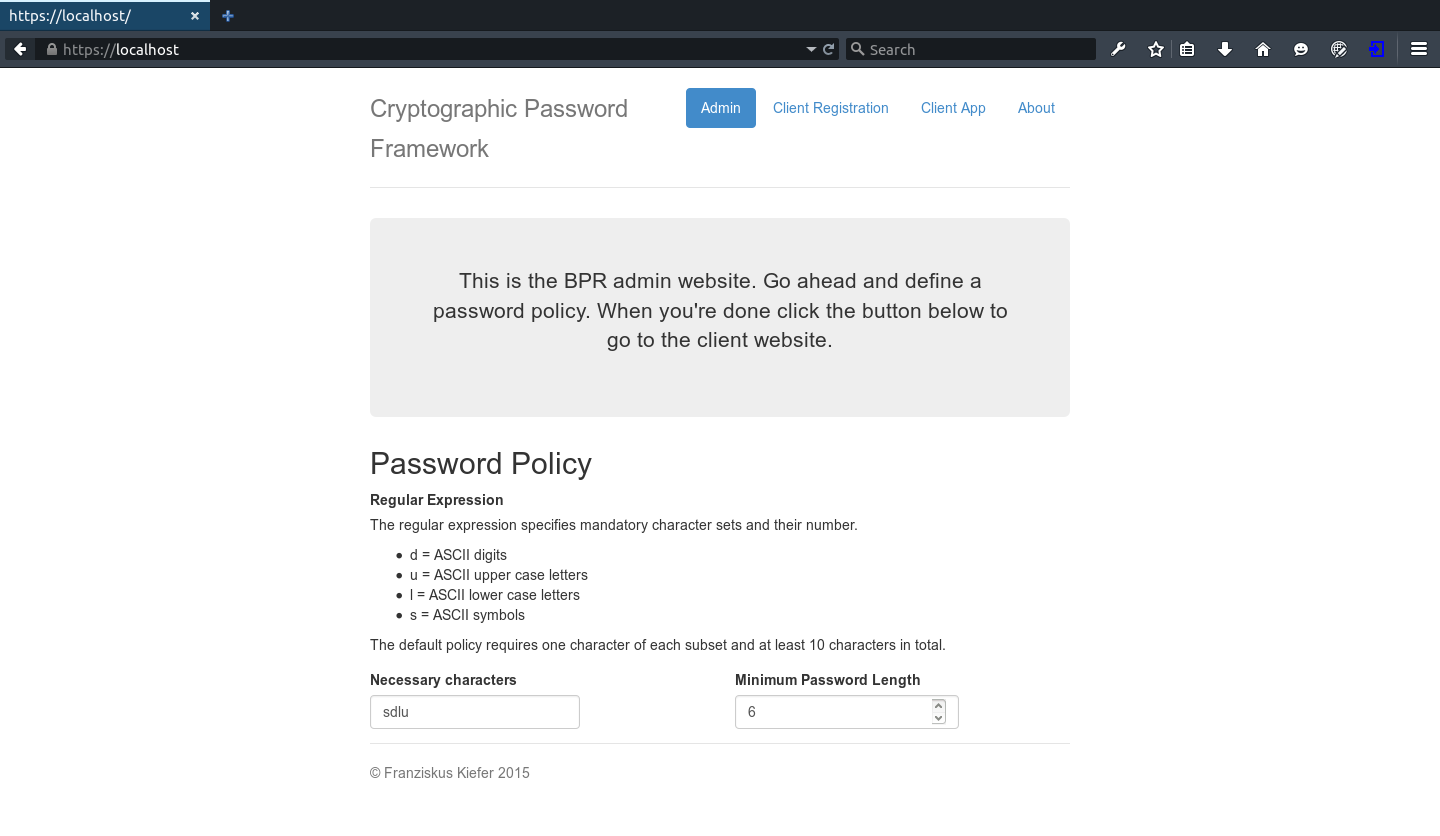
\includegraphics[width=0.98\textwidth]{Figs/demo-admin.png}
\caption{Demo --- Admin interface}\label{fig:demo-admin}
\end{figure}

\paragraph{Client Interface}
Selecting the \emph{Client Registration} link presents the user with a simple website asking the user to register a new user and password.
To this end the user has to click the registration/login button in the browser toolbar to open the registration form.
This button is only active for websites that support the \ac{BPR} registration process and provides the user with a trusted path to a trusted registration form.
Note that it is important that the registration form is trusted and \emph{not} provided by the server as the server is not trusted with secure handling of the client password.
After clicking ``Register Now'' the extension performs the \ac{BPR} protocol from Section \ref{sec:bpr} with the server.
The JavaScript implementation makes use of cryptographic libraries\footnote{\url{http://www-cs-students.stanford.edu/~tjw/jsbn/},\\\hspace*{1.5em} \url{https://github.com/bitwiseshiftleft/sjcl}}), while the server uses the Charm library by \citet{charm13}.

\begin{figure}[tbph]
\centering
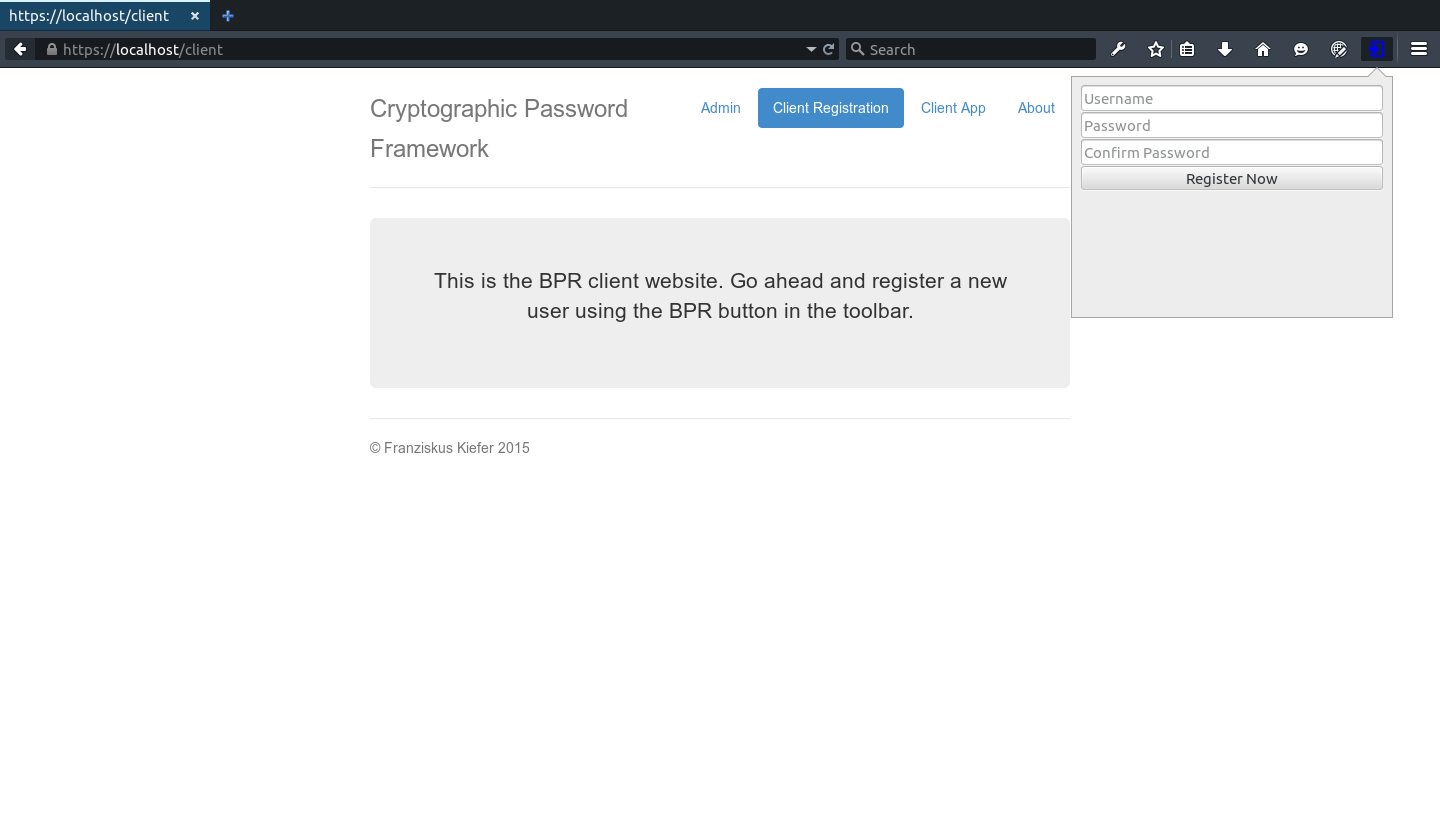
\includegraphics[width=0.98\textwidth]{Figs/demo-register-popup.png}
\caption{Demo --- Client Registration interface}\label{fig:demo-register}
\end{figure}

\subsection{Login}
Clicking on the ``Client App'' link provides the user with a simple website asking the user to log into the application using the registration/login button in the browser toolbar.
Similar to the registration process, the user is presented with a trusted login form.
After entering user name and password, and clicking ``Login'', the extension performs the tSoke protocol with the server.
As discussed before, tSoke is a \ac{VPAKE} protocol that additionally uses a tag to make it usable in the \ac{PACCE} setting.
Thereby, client and server perform a \ac{PACCE} protocol, which hands the session over to the client application when done.

\begin{figure}[tbph]
\centering
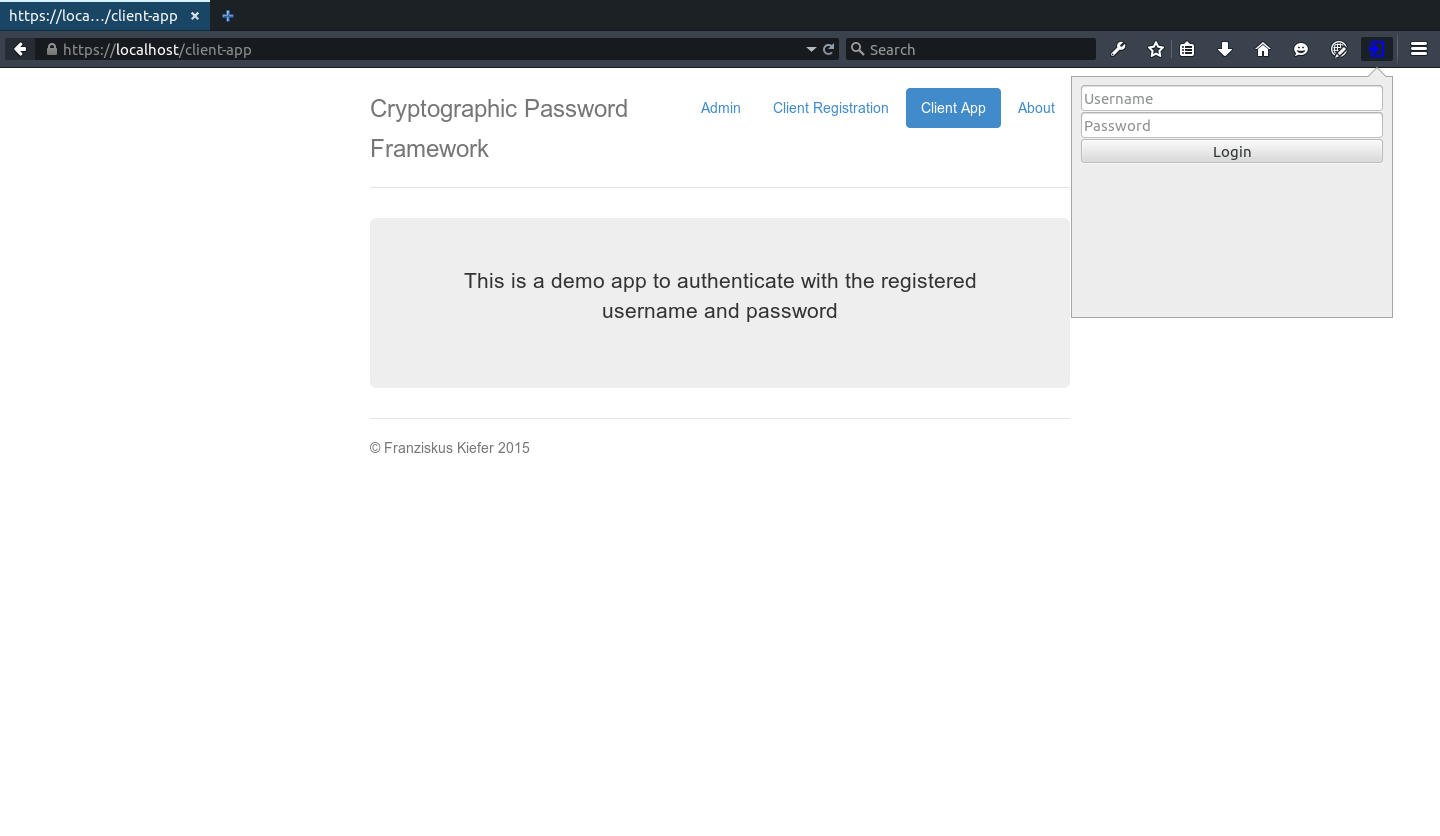
\includegraphics[width=0.98\textwidth]{Figs/demo-login-popup.png}
\caption{Demo --- Client Login interface}\label{fig:demo-login}
\end{figure}

\subsection{Demo Application}
The client demo application, a simple to-do application, is depicted in Figure \ref{fig:demo-app}.
It is an independent component and embedded in the framework website as an iframe.
It uses NodeJS\footnote{\url{https://nodejs.org/}} as RESTful\footnote{\url{https://en.wikipedia.org/wiki/Representational_state_transfer}} server, MongoDB\footnote{\url{https://www.mongodb.org/}} for storage, and jade\footnote{\url{http://jade-lang.com/}} as template engine.

\begin{figure}[tbph]
\centering
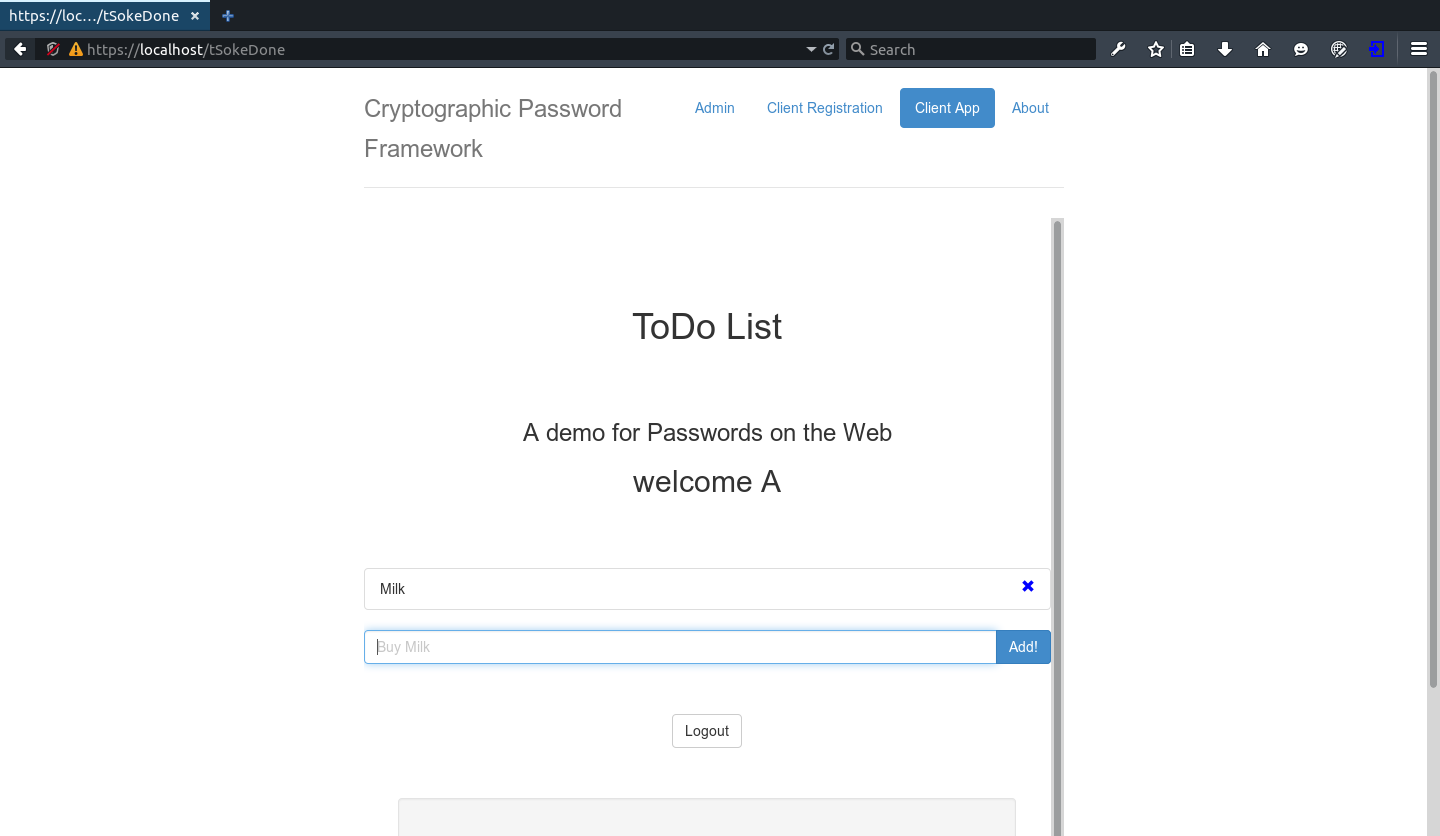
\includegraphics[width=0.98\textwidth]{Figs/demo-app.png}
\caption{Demo --- Client Application interface}\label{fig:demo-app}
\end{figure}


% \section{Extending the Framework -- Oblivious VPAKE}
% \mynote{OVPAKE for password trials \cite{Kiefer2012,Kiefer13a} (not implemented)}

\section{Conclusion} \label{sec:vpake-conclusion}
This chapter proposed a password registration and authentication framework for the single server setting, gave efficient instantiation and a demo application to show its use.
Using \ac{ZKPPC} as basis, Section \ref{sec:bpr} proposed an efficient \acl{BPR} protocol with security model.
An alternative approach to the problem of \ac{BPR} is proposed in Section \ref{sec:spc-bpr} using set theory.
Comparison of the two proposed \ac{BPR} protocols show that the set-based approach is significantly faster due to the use of symmetric primitives, while requiring a different security model.
The second step in the framework, password-based authentication, is solved by a new \ac{VPAKE} protocol in Section \ref{sec:vpake}.
Implementation (Section \ref{sec:discussion}) and demonstration (Section \ref{sec:vpake-demo}) showed practicability of the proposed approach.
